\section{MÓDULO 1: CORRIDA DOS
NÚMEROS}\label{muxf3dulo-1-corrida-dos-nuxfameros}

Neste módulo vamos trabalhar com os alunos as habilidades referentes à
manipulação dos algarismos, de modo que o aluno consiga formar, ordenar
e utilizar alguns números, de até 3 ordens, em diversas aplicações de
contagem, ordenação e identificação.

Habilidades da BNCC: EF01MA01, EF01MA03 e EF01MA05

HABILIDADES DO SAEB

\begin{itemize}
\item
  Reconhecer o que os números naturais indicam em diferentes situações:
  quantidade, ordem, medida ou código de identificação.
\item
  Identificar a posição ordinal de um objeto ou termo em uma sequência
  (1º, 2º etc.).
\item
  Escrever números naturais de até 3 ordens em sua representação por
  algarismos ou em língua materna ou associar o registro numérico de
  números naturais de até 3 ordens ao registro em língua materna.
\item
  Comparar ou ordenar quantidades de objetos (até 2 ordens).
\item
  Comparar ou ordenar números naturais de até 3 ordens com ou sem
  suporte da reta numérica.
\item
  Identificar a ordem ocupada por um algarismo ou seu valor posicional
  (ou valor relativo) em um número natural de até 3 ordens.
\end{itemize}

\subsection{CONTEÚDO}\label{conteuxfado}

Os amigos do condomínio de joão resolveram fazer umA CORRIDA COM SEUS
CARRINHOS. HAVIAM \textbf{QUINZE} GAROTOS, E CADA UM DELES TROUXE
\textbf{UM} CARRINHO PARA A CORRIDA. QUEM SERÁ QUE CHEGARÁ EM
\textbf{PRIMEIRO} LUGAR? QUEM SERÁ QUE CHEGARÁ EM \textbf{SEGUNDO}
LUGAR? e QUEM COMPLETARÁ O PÓDIO CHEGANDO EM \textbf{TERCEIRO} LUGAR?
PARA MELHORAR O CONTROLE DA CORRIDA, OS MENINOS RESOLVERAM CODIFICAR
CADA CARRINHO COM UM NÚMERO. JOÃO, QUE FOI QUEM TEVE A IDEIA DA CORRIDA,
TRATOU LOGO DE ESCOLHER O NÚMERO DE SEU PILOTO FAVORITO DE FORMULA 1. OS
OUTROS MENINOS ESCOLHERAM NÚMEROS QUE ELES GOSTAVAM. TINHA O CARRO
\textbf{44}, TINHA O CARRO \textbf{12}, ENTRE OUTROS.

\textless{}Verificar a possibilidade de uso da referência:
https://br.freepik.com/vetores-gratis/cinco-criancas-correndo-em-um-carro
juntas\_19796038.htm\#query=CARRINHOS\%20DE\%20CORRIDA\&position=26\&from\_view=search\&track=ais\textgreater{}

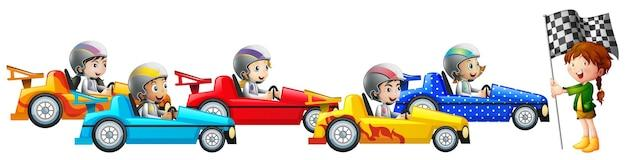
\includegraphics[width=4.15174in,height=1.06137in]{media/image1.jpg}

Você percebeu como usamos os números de diversas formas? eles foram
úteis para NOS AJUDAR A CONTAR OS CARROS E A QUANTIDADE DE PARTICIPANTES
DA CORRIDA, ELES TAMBÉM NOS AJUDARAM A DEFINIR A CLASSIFICAÇÃO DOS
CORREDORES, E ATÉ NOS INDICARÁ O VENCEDOR, OU SEJA, O PRIMEIRO A CRUZAR
A LINHA DE CHEGADA. ALÉM DISSO, OS NÚMEROS NÃO SERVEM SOMENTE PARA
CONTARMOS COISAS, MAS TAMBÉM PARA IDENTIFICARMOS ESSAS MESMAS COISAS. OS
NOSSOS AMIGOS CORREDORES DERAM NÚMEROS DE IDENTIFICAÇÃO AOS SEUS CARROS.
nOSSAS CASAS TAMBÉM TÊM NÚMEROS. lEMBRAM? eSSE É MAIS UM EXEMPLO DE
NÚMEROS IDENTIFICANDO COISAS AO INVÉS DE CONTANDO.

\subsection{ATIVIDADES}\label{atividades}

\subsubsection{1. CIRCULE A FIGURA QUE CONTÉM UM NÚMERO USADO COMO
CÓDIGO DE
IDENTIFICAÇÃO.}\label{circule-a-figura-que-contuxe9m-um-nuxfamero-usado-como-cuxf3digo-de-identificauxe7uxe3o.}

\textless{}https://stock.adobe.com/br/images/id/363300782?get\_facets=1\&order=relevance\&safe\_search=1\&k=r\%C3\%A9gua\&clickref=1100lwwNzM24\&mv=affiliate\&mv2=Freepik\&as\_camptype=\&as\_channel=affiliate\&as\_source=partnerize\&as\_campaign=Freepik\&as\_content=api\&as\_audience=srp\&sdid=6WTV6YJ5;
https://stock.adobe.com/br/search?load\_type=search\&is\_recent\_search=\&search\_type=usertyped\&k=NUMERO+DE+CASA\&native\_visual\_search=\&similar\_content\_id=\&asset\_id=506848063;
https://stock.adobe.com/br/search?filters\%5Bcontent\_type\%3Aphoto\%5D=1\&filters\%5Bcontent\_type\%3Aillustration\%5D=1\&filters\%5Bcontent\_type\%3Azip\_vector\%5D=1\&filters\%5Bcontent\_type\%3Avideo\%5D=1\&filters\%5Bcontent\_type\%3Atemplate\%5D=1\&filters\%5Bcontent\_type\%3A3d\%5D=1\&filters\%5Bcontent\_type\%3Aimage\%5D=1\&order=relevance\&safe\_search=1\&limit=100\&search\_page=1\&k=1+KG\&search\_type=usertyped\&acp=\&aco=1+KG\&get\_facets=0\&asset\_id=418803262.
Inserir um diagrama com as 4 figuras, conforme modelo a seguir. É
importante que as imagens tenham um tamanho grande, para que os alunos
consigam enxergar os números.\textgreater{}

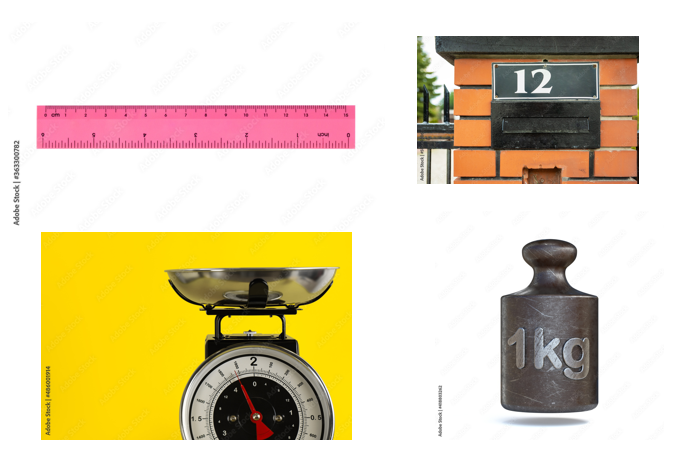
\includegraphics[width=3.98893in,height=2.65350in]{media/image2.png}

Professor(a), em todas as outras figuras os números são usados para
quantificar medidas. Somente na figura da caixa de correio encontramos
um número identificador.

\subsubsection{2. INDIQUE OS NÚMEROS DOS CARROS NA POSIÇÃO EM QUE
CRUZARAM A LINHA DE CHEGADA. NINGUÉM ULTRAPASSOU NINGUÉM!
}\label{indique-os-nuxfameros-dos-carros-na-posiuxe7uxe3o-em-que-cruzaram-a-linha-de-chegada.-ninguuxe9m-ultrapassou-ninguuxe9m}

\textless{}Inserir o diagrama a seguir conforme modelo. Licenciar a
figura:
https://br.freepik.com/vetores-gratis/no-jogo-de-corrida-de-velocidade-o-jogador-do-driver-do-monstro-da-competicao-usou-o-carro-de-alta-velocidade-para-vencer-no-jogo\_16304604.htm\#query=carros\%20com\%20n\%C3\%BAmeros\&position=11\&from\_view=search\&track=ais.\textgreater{}

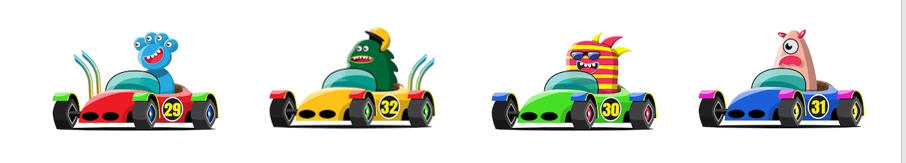
\includegraphics[width=5.90556in,height=1.06250in]{media/image3.png}

\textless{}Criar uma figura de um podium, com círculos acima das
posições, onde os alunos colocarão os números dos carros.\textgreater{}

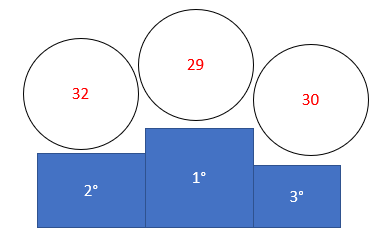
\includegraphics[width=3.92763in,height=2.54202in]{media/image4.png}

Professor(a), oriente os alunos acerca das funções dos números de
identificação dos carros, destacando que eles não são os números que
indicarão a ordem de chegada deles. Oriente-os para que entendam que a
ordem se inicia da esquerda para a direita.

\subsubsection{3. LIGUE OS NÚMEROS CORRETAMENTE
}\label{ligue-os-nuxfameros-corretamente}

\begin{longtable}[]{@{}ll@{}}
\toprule
326 & Cem\tabularnewline
100 & cento e cinquenta e quatro\tabularnewline
154 & cento e cinquenta\tabularnewline
451 & quatrocentos e quinze\tabularnewline
514 & seiscentos e vinte e três\tabularnewline
150 & quinhentos e quatorze\tabularnewline
415 & trezentos e vinte e seis\tabularnewline
623 & quatrocentos e cinquenta e um\tabularnewline
\bottomrule
\end{longtable}

Professor(a) oriente os alunos a encontrarem os números representados
por algarismos correspondentes aos números representados por textos.

\subsubsection{4. ALBERTO TEM UMA COLEÇÃO DE CAMISAS DE FUTEBOL. JÚNIOR
TEM UMA COLEÇÃO DE BOLAS. QUAL DAS DUAS COLEÇÕES É A MAIOR?
}\label{alberto-tem-uma-coleuxe7uxe3o-de-camisas-de-futebol.-juxfanior-tem-uma-coleuxe7uxe3o-de-bolas.-qual-das-duas-coleuxe7uxf5es-uxe9-a-maior}

\textless{}Inserir figuras:
https://br.freepik.com/vetores-gratis/time-de-futebol-ou-jogadores-de-time-de-futebol-em-fundo-branco\_10600572.htm\#query=cole\%C3\%A7\%C3\%A3o\%20de\%20figurinhas\&position=11\&from\_view=search\&track=ais;
https://br.freepik.com/vetores-gratis/bolas-definir-ilustracao-vetorial\_4559016.htm\#query=cole\%C3\%A7\%C3\%A3o\%20de\%20bolas\&position=0\&from\_view=search\&track=ais.
Não precisa traduzir os textos em inglês, pois eles não são necessários
à resolução.\textgreater{}

\begin{quote}
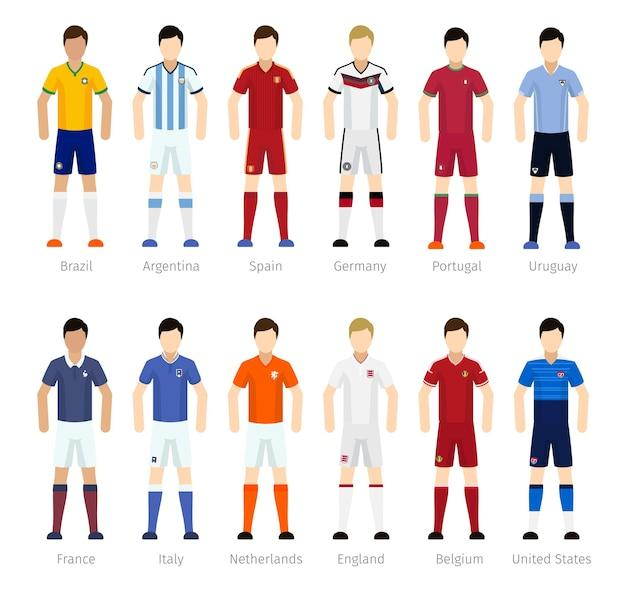
\includegraphics[width=2.90024in,height=2.77508in]{media/image5.jpg}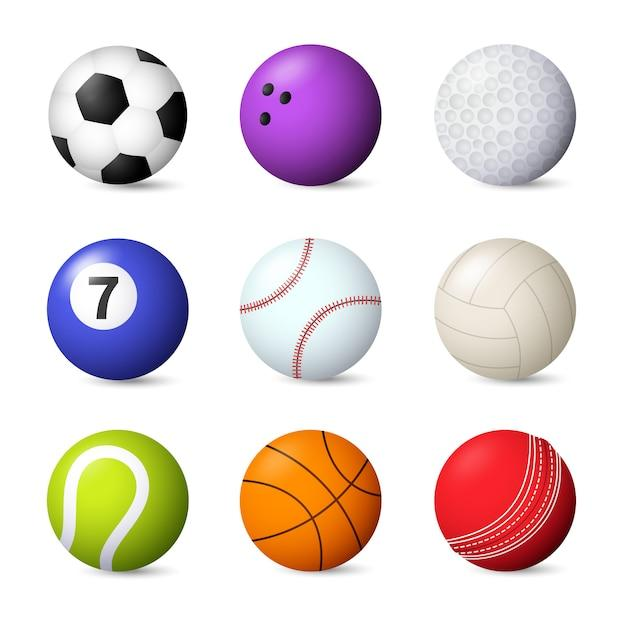
\includegraphics[width=2.59375in,height=2.59375in]{media/image6.jpg}
\end{quote}

O aluno deve contar as duas coleções e perceber que a coleção de camisas
de Alberto é maior, pois tem mais unidades do que a coleção de Junior.

\subsubsection{5. RESPONDA MAIS PERGUNTAS SOBRE A ATIVIDADE
ANTERIOR}\label{responda-mais-perguntas-sobre-a-atividade-anterior}

\begin{enumerate}
\def\labelenumi{\Alph{enumi})}
\item
  Quantas camisas alberto tem? \textless{}1 linha\textgreater{}
\end{enumerate}

12 camisas.

\begin{enumerate}
\def\labelenumi{\Alph{enumi})}
\item
  Quantas bolas junior tem? \textless{}1 linha\textgreater{}
\end{enumerate}

9 bolas.

\begin{enumerate}
\def\labelenumi{\Alph{enumi})}
\item
  quantos itens a mais que junior, alberto tem em sua coleção?
  \textless{}1 linha\textgreater{}
\end{enumerate}

3 itens.

\subsubsection{6. CIRCULE O CONJUNTO DE DADOS COM O MAIOR
RESULTADO}\label{circule-o-conjunto-de-dados-com-o-maior-resultado}

\textless{} Inserir um quadro com as imagens conforme o modelo a seguir.
https://br.freepik.com/vetores-gratis/dados-isometricos-cubos-de-jogo-pretos-variantes-isolados-no-fundo-branco-coleta-de-todas-as-voltas-possiveis\_13090027.htm\#query=dice\&position=1\&from\_view=search\&track=sph.\textgreater{}

\begin{longtable}[]{@{}ll@{}}
\toprule
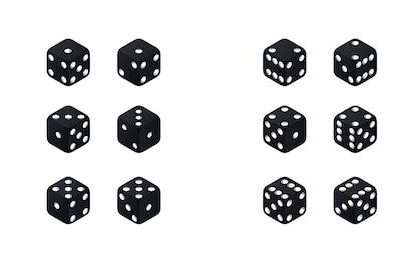
\includegraphics[width=1.85846in,height=2.68750in]{media/image7.jpg} &
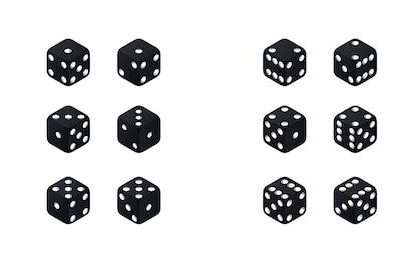
\includegraphics[width=1.57843in,height=2.68750in]{media/image7.jpg}\tabularnewline
\bottomrule
\end{longtable}

Professor(a), oriente os alunos a olharem para o resultado da face
superior do dado. Da mesma forma como eles fariam ao jogar um joguinho
de tabuleiro. A figura que deve ser circulada é a figura da direita,
pois a soma de seus dados é maior do que a soma dos dados da esquerda.

\subsubsection{7. APROVEITANDO A ATIVIDADE
ANTERIOR:}\label{aproveitando-a-atividade-anterior}

A. PINTE DE AZUL O QUADRADINHO QUE TEM O NÚMERO DA SOMA DOS DADOS DA
DIREITA

B. PINTE DE VERDE O QUADRADINHO QUE TEM O NÚMERO DA SOMA DOS DADOS DA
ESQUERDA

C. PINTE DE AMARELO A DIFERENÇA ENTRE AS DUAS SOMAS.

\begin{longtable}[]{@{}lllll@{}}
\toprule
12 & 24 & 30 & 40 & 10\tabularnewline
6 & 21 & 20 & 8 & 5\tabularnewline
7 & 18 & 4 & 22 & 13\tabularnewline
19 & 2 & 1 & 23 & 15\tabularnewline
25 & 11 & 9 & 17 & 32\tabularnewline
\bottomrule
\end{longtable}

O aluno deve pintar o número 18 de verde, o número 22 de azul e o número
4 de amarelo.

\subsubsection{8. ESCREVA OS SEGUINTES NÚMEROS EM ORDEM
CRESCENTE}\label{escreva-os-seguintes-nuxfameros-em-ordem-crescente}

516 -- 645 -- 215 -- 326 - 789

\begin{longtable}[]{@{}lllll@{}}
\toprule
215 & 326 & 516 & 645 & 789\tabularnewline
\bottomrule
\end{longtable}

132 -- 165 -- 112 -- 115 -- 100

\begin{longtable}[]{@{}lllll@{}}
\toprule
100 & 112 & 115 & 132 & 165\tabularnewline
\bottomrule
\end{longtable}

325 -- 854 -- 127 -- 974 -- 546

\begin{longtable}[]{@{}lllll@{}}
\toprule
127 & 325 & 546 & 854 & 974\tabularnewline
\bottomrule
\end{longtable}

415 -- 418 -- 411 -- 410 -- 417

\begin{longtable}[]{@{}lllll@{}}
\toprule
410 & 411 & 415 & 417 & 418\tabularnewline
\bottomrule
\end{longtable}

798 -- 987 -- 879 -- 897 -- 978

\begin{longtable}[]{@{}lllll@{}}
\toprule
798 & 879 & 897 & 978 & 987\tabularnewline
\bottomrule
\end{longtable}

623 -- 236 -- 362 -- 326 -- 263

\begin{longtable}[]{@{}lllll@{}}
\toprule
236 & 263 & 326 & 362 & 623\tabularnewline
\bottomrule
\end{longtable}

\subsubsection{9. ESCREVA OS SEGUINTES NÚMEROS EM ORDEM
DECRESCENTE}\label{escreva-os-seguintes-nuxfameros-em-ordem-decrescente}

564 -- 456 -- 546 -- 645 -- 465

\begin{longtable}[]{@{}lllll@{}}
\toprule
645 & 564 & 546 & 465 & 456\tabularnewline
\bottomrule
\end{longtable}

138 -- 831 -- 318 -- 183 -- 813

\begin{longtable}[]{@{}lllll@{}}
\toprule
831 & 813 & 318 & 183 & 138\tabularnewline
\bottomrule
\end{longtable}

715 -- 517 -- 751 -- 571 -- 175

\begin{longtable}[]{@{}lllll@{}}
\toprule
751 & 715 & 571 & 517 & 175\tabularnewline
\bottomrule
\end{longtable}

833 -- 383 -- 838 -- 338 -- 388

\begin{longtable}[]{@{}lllll@{}}
\toprule
838 & 833 & 388 & 383 & 338\tabularnewline
\bottomrule
\end{longtable}

717 -- 177 -171 -- 117 -- 771

\begin{longtable}[]{@{}lllll@{}}
\toprule
771 & 717 & 177 & 171 & 117\tabularnewline
\bottomrule
\end{longtable}

100 -- 200 -- 300 - 400 -- 500

\begin{longtable}[]{@{}lllll@{}}
\toprule
500 & 400 & 300 & 200 & 100\tabularnewline
\bottomrule
\end{longtable}

\subsubsection{10. JERÔNIMO MORA NA CASA 328 DA RUA SANTOS, EM SUA
CIDADE. LIGUE CORRETAMENTE OS ALGARISMOS DO NÚMERO DA CASA ÀS ORDENS
CORRESPONDENTES}\label{jeruxf4nimo-mora-na-casa-328-da-rua-santos-em-sua-cidade.-ligue-corretamente-os-algarismos-do-nuxfamero-da-casa-uxe0s-ordens-correspondentes}

\begin{longtable}[]{@{}ll@{}}
\toprule
3 & dezenas\tabularnewline
2 & centenas\tabularnewline
8 & unidades\tabularnewline
\bottomrule
\end{longtable}

\subsubsection{11. PINTE OS QUADRADOS COM A COR DA ORDEM CORRESPONDENTE
}\label{pinte-os-quadrados-com-a-cor-da-ordem-correspondente}

\textless{}Criar um afigura conforme o modelo a seguir.\textgreater{}

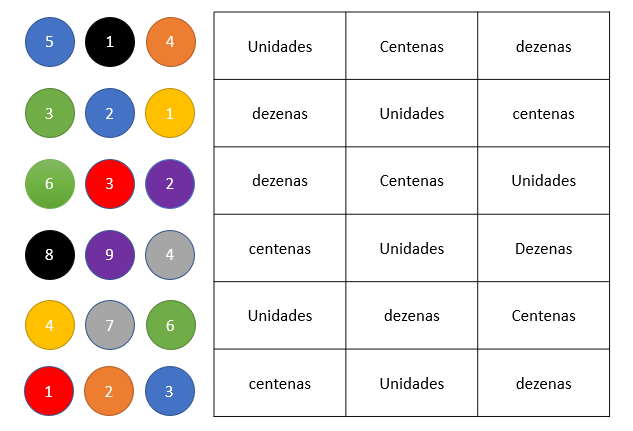
\includegraphics[width=5.90556in,height=4.02083in]{media/image8.png}

Professor(a), oriente os alunos a pintarem as cores das ordens nos
respectivos quadradinhos indicados.

\begin{longtable}[]{@{}lll@{}}
\toprule
laranja & azul & Preto\tabularnewline
azul & amarelo & Verde\tabularnewline
vermelho & verde & Roxo\tabularnewline
preto & cinza & Roxo\tabularnewline
verde & cinza & Amarelo\tabularnewline
vermelho & azul & Laranja\tabularnewline
\bottomrule
\end{longtable}

\subsubsection{12. }\label{section}

Os três competidores da figura estão no \emph{podium}. ELES TÊM os nomes
escritos na camiseta. descubra qual a pontuação de cada um deles,
escrevendo seus nomes na tabela.

\textless{}Inserir a figura de referência:
https://br.freepik.com/vetores-gratis/podio-esportes\_1040693.htm\#query=podium\%20com\%20competidores\&position=1\&from\_view=search\&track=ais.
Acrescente os nomes dos competidores, conforme o modelo a
seguir.\textgreater{}

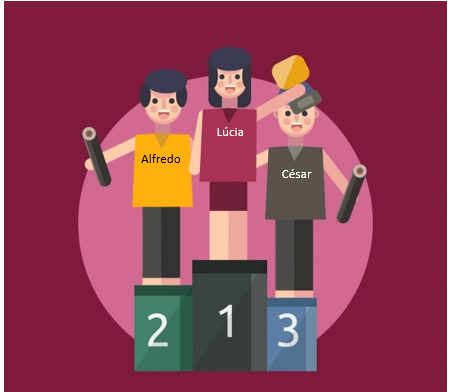
\includegraphics[width=3.84950in,height=3.34590in]{media/image9.png}

\begin{longtable}[]{@{}ll@{}}
\toprule
\textbf{Pontos} & \textbf{nomes}\tabularnewline
1~000 pontos & César\tabularnewline
1~005 pontos & Lúcia\tabularnewline
1~0004 pontos & Alfredo\tabularnewline
\bottomrule
\end{longtable}

Professor(a), é importante que os alunos compreendam que o primeiro
colocado deve ter feito a maior quantidade de pontos, e assim por
diante.

\subsubsection{13 }\label{section-1}

a reta numerada abaixo representa uma rua qualquer de um bairro. Ligue
as casas às suas respectivas posições conforme o seu número.

\textless{}Criar uma reta numérica conforme o modelo a seguir. Depois
colocar a figura de referência:
https://br.freepik.com/vetores-gratis/pacote-de-belas-fachadas-de-casas-desenhadas-a-mao\_1198631.htm\#page=2\&query=casas\%20coloridas\&position=11\&from\_view=search\&track=ais
com os respectivos números conforme o modelo.

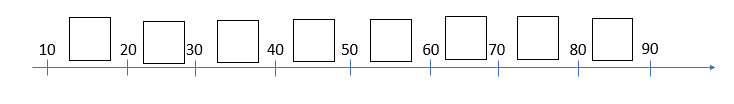
\includegraphics[width=5.90556in,height=0.83681in]{media/image10.png}

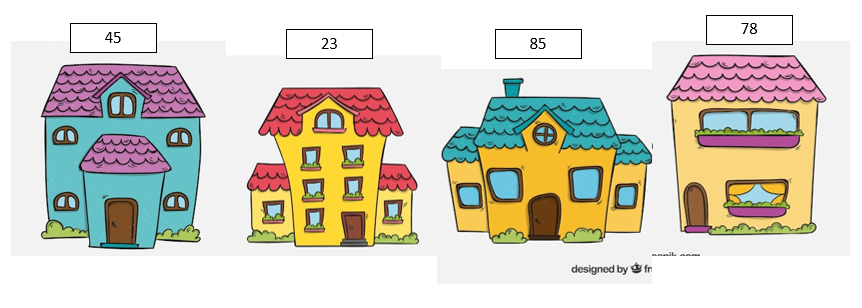
\includegraphics[width=5.90556in,height=2.10972in]{media/image11.png}

\subsubsection{14}\label{section-2}

Escreva os numeros a seguir com algarismos.

\begin{longtable}[]{@{}ll@{}}
\toprule
Seiscentos e dezenove & 619\tabularnewline
oitocentos e trinta e sete & 837\tabularnewline
novecentos e quarenta e um & 941\tabularnewline
cento e dois & 102\tabularnewline
cento e trinta e oito & 138\tabularnewline
duzentos e vinte e cinco & 225\tabularnewline
trezentos e oitenta e quatro & 384\tabularnewline
quatrocentos e quinze & 415\tabularnewline
quinhentos e setenta e sete & 577\tabularnewline
setecentos e dezesseis & 716\tabularnewline
cento e cinquenta e três & 153\tabularnewline
\bottomrule
\end{longtable}

\subsubsection{}\label{section-3}

\subsection{TREINO}\label{treino}

\subsubsection{01 }\label{section-4}

na carteirinha da escola de júlia tem sua foto, seu nome e o número do
seu registro de matrícula. no caso de julia esse número é o 363. qual o
tipo de situação que esse número indica?

\begin{enumerate}
\def\labelenumi{\Alph{enumi})}
\item
  quantidade
\item
  ordem
\item
  medida
\item
  código de identificação
\end{enumerate}

SAEB: 2N1.1 Reconhecer o que os números naturais indicam em diferentes
situações: quantidade, ordem, medida ou código de identificação.

BNCC: (EF01MA01) Utilizar números naturais como indicador de quantidade
ou de ordem em diferentes situações cotidianas e reconhecer situações em
que os números não indicam contagem nem ordem, mas sim código de
identificação.

\begin{enumerate}
\def\labelenumi{\alph{enumi})}
\item
  Incorreta. O número apresentado não representa quantidade ou contagem.
\item
  Incorreta. O número apresentado não apresenta necessariamente a ordem
  de matriculas feitas na escola
\item
  Incorreta. O número não representa nenhuma unidade como metro ou
  grama.
\item
  Correta. Esse número é um código de identificação da aluna Júlia nos
  registros da escola.
\end{enumerate}

\subsubsection{02 }\label{section-5}

A figura mostra quatro coleções de amigos que gostam de colecionar
bolinhas de gude.

\textless{}Criar a figura conforme modelo a seguir.\textgreater{}

\begin{quote}
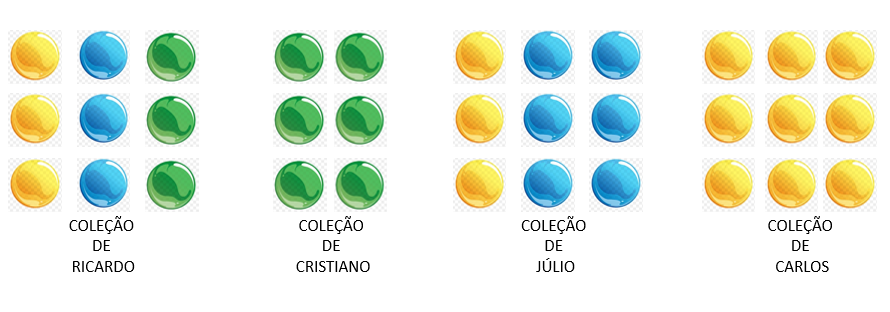
\includegraphics[width=5.90556in,height=2.07014in]{media/image12.png}
\end{quote}

qual coleção tem a maior quantidade de bolas de um única cor?

\begin{enumerate}
\def\labelenumi{\Alph{enumi})}
\item
  carlos
\item
  cristiano
\item
  júlio
\item
  ricardo
\end{enumerate}

SAEB: 2N1.4 Comparar OU ordenar quantidade de objetos (até 2 ordens).

BNCC: (EF01MA05) Comparar números naturais de até duas ordens em
situações cotidianas, com e sem suporte da reta numérica.

\begin{enumerate}
\def\labelenumi{\alph{enumi})}
\item
  Correta. Carlos tem a mesma quantidade de bolas de alguns amigos,
  porém, todas são amarelas.
\item
  Incorreta. Cristiano só tem bolas verdes, porém, tem menos bolas do
  que Carlos
\item
  Incorreta. Júlio tem bastante bolas azuis, porém, em menor quantidade
  do que as bolas amarelas de Carlos
\item
  Incorreta. Ricardo tem poucas bolas de cada cor, apesar de ter o mesmo
  número total de bolas do que Carlos.
\end{enumerate}

\subsubsection{03 }\label{section-6}

entre 0 e 100, quantos números terminam com o número zero na ordem das
unidades?

\begin{enumerate}
\def\labelenumi{\Alph{enumi})}
\item
  1
\item
  9
\item
  10
\item
  11
\end{enumerate}

SAEB: 2N1.6 -- Identificar a ordem ocupada por um algarismo OU seu valor
posicional (ou valor relativo) em um número natural de até 3 ordens.

BNCC: (EF01MA03) Estimar e comparar quantidades de objetos de dois
conjuntos (em torno de 20 elementos), por estimativa e/ou por
correspondência (um a um, dois a dois) para indicar ``tem mais'', ``tem
menos'' ou ``tem a mesma quantidade''.

\begin{enumerate}
\def\labelenumi{\alph{enumi})}
\item
  Incorreta. O aluno pode ter considerado somente o zero, entendendo que
  era só algarismos na ordem das unidades
\item
  Incorreta. O aluno pode ter esquecido de considerar o zero \textbf{E}
  o cem.
\item
  Incorreta. O aluno pode ter esquecido de considerar o zero \textbf{OU}
  o cem.
\item
  Correta. O aluno contou os números: 0,10, 20, 30, 40, 50, 60, 70, 80,
  90 e 100.
\end{enumerate}

\section{\texorpdfstring{\\
}{ }}\label{section-7}

\section{MÓDULO 2: JUNTAR OU TIRAR?}\label{muxf3dulo-2-juntar-ou-tirar}

Neste módulo vamos desenvolver a habilidade de desenvolvimento de
cálculos, tanto no sentido de escolher a melhor estratégia, como no
sentido de resolver o problema. Faremos essa abordagem de forma
abstrata, mas também de forma contextualizada, com o fim de desenvolver
nos alunos a motivação para resolverem problemas reais.

Habilidades do SAEB:

- Calcular o resultado de adições e subtrações, envolvendo número
naturais de até 3 ordens.

- Compor ou decompor números naturais de até 3 ordens por meio de
diferentes adições.

- Resolver problemas de adição ou de subtração, envolvendo números
naturais de até 3 ordens, com os significados de juntar, acrescentar,
separar ou retirar.

\subsection{CONTEÚDO}\label{conteuxfado-1}

A mamãe ou oi papai já te deram mesada alguma vez? aí você ficou todo
feliz e decidiu que queria comprar alguma coisa. O que você pensou em
comprar? doces? figurinhas? algum brinquedo?

márcia ganhou de seu papai duas notas de dez reais. ela decidiu que
queria comprar um brinquedo que custava quinze reais. márcia percebeu
que tinha um problema: para saber se ela teria condições de comprar
aquele brinquedo, ela teria que descobrir quanto dinheiro tinha. o papai
dela resolveu ajudar. ele pegou a quantidade de palitos equivalente as
notas. observe:

\textless{}Criar uma ilustração com duas carreiras de 10 palitos
alinhadas a uma cédula de 10 reais, conforme o modelo a seguir.
https://www.istockphoto.com/br/foto/dez-real-brasileiro-gm181402095-26926813?utm\_campaign=srp\_photos\_inline\&utm\_content=https\%3A\%2F\%2Fwww.pexels.com\%2Fprocurar\%2F10\%2520reais\%2F\&utm\_medium=affiliate\&utm\_source=pexels\&utm\_term=10+reais

https://br.freepik.com/fotos-premium/uma-partida-com-cabeca-verde-em-um-fundo-branco\_31512045.htm\#page=3\&query=palito\%20de\%20f\%C3\%B3sforo\&position=18\&from\_view=search\&track=ais\textgreater{}

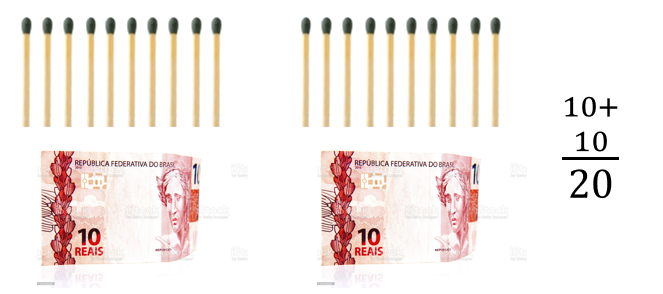
\includegraphics[width=3.31224in,height=1.46877in]{media/image13.png}

márcia contou os palitos e percebeu que tinha 20 reais. agora, ela
precisava saber se esses 20 reais seriam suficientes para comprar o
brinquedo. a propria márcia pegou mais quinze palitinhos e os alinhou da
seguinte forma:

\textless{}Criar uma figura com duas linhas de palito alinhados. Na
primeira linha 20 e na segunda linha 15. Colocar a operação ao lado,
conforme modelo a seguir.\textgreater{}

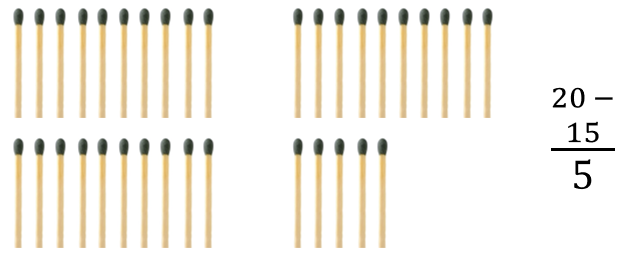
\includegraphics[width=3.31185in,height=1.38526in]{media/image14.png}

márcia ficou muito feliz ao perceber que poderia comprar seu brinquedo,
e ainda lhe sobrariam cinco reais para comprar doces. que dia gostoso
teve márcia!

\subsection{ATIVIDADES}\label{atividades-1}

\subsubsection{1}\label{section-8}

pinte o foguete com as cores corretas. descubra as cores resolvendo as
adições.

\textless{}Inserir um quadro conforme o modelo a seguir.
https://br.freepik.com/vetores-premium/foguete-de-desenho-bonito-de-cor-planilha-para
criancas\_22159996.htm\#page=6\&query=para\%20colorir\%20foguete\&position=7\&from\_view=search\&track=ais.\textgreater{}

\begin{longtable}[]{@{}lll@{}}
\toprule
59 & &
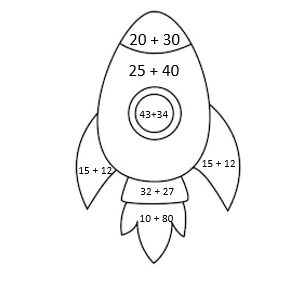
\includegraphics[width=3.09611in,height=2.97268in]{media/image15.png}\tabularnewline
65 & &\tabularnewline
77 & &\tabularnewline
90 & &\tabularnewline
50 & &\tabularnewline
27 & &\tabularnewline
\bottomrule
\end{longtable}

Professor(a), oriente os alunos a resolverem as adições primeiro, antes
de começarem a pintar o foguete. No quadro a esquerda, temos as
resoluções das adições, onde o aluno deve pintar o pedaço do foguete com
a cor correspondente.

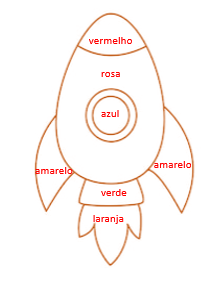
\includegraphics[width=1.43098in,height=1.89472in]{media/image16.png}

\subsubsection{2}\label{section-9}

efetue as adições a seguir:

\begin{longtable}[]{@{}llllllllll@{}}
\toprule
51 & + & 32 & + & 13 & + & 74 & + & 23 & +\tabularnewline
12 & & 21 & & 15 & & 20 & & 31 &\tabularnewline
63 & & 53 & & 28 & & 94 & & 54 &\tabularnewline
\bottomrule
\end{longtable}

\begin{longtable}[]{@{}llllllllll@{}}
\toprule
24 & + & 41 & + & 11 & + & 10 & + & 29 & +\tabularnewline
13 & & 36 & & 11 & & 60 & & 15 &\tabularnewline
37 & & 77 & & 22 & & 70 & & 44 &\tabularnewline
\bottomrule
\end{longtable}

Professor(a), oriente os alunos a iniciarem as adições pela ordem das
unidades, seguindo pela ordem das dezenas, e finalmente a das centenas
para obter o resultado.

\subsubsection{3}\label{section-10}

efetue as subtrações a seguir

\begin{longtable}[]{@{}llllllllll@{}}
\toprule
51 & - & 32 & - & 15 & - & 74 & - & 31 & -\tabularnewline
12 & & 21 & & 13 & & 20 & & 23 &\tabularnewline
39 & & 11 & & 2 & & 54 & & 8 &\tabularnewline
\bottomrule
\end{longtable}

\begin{longtable}[]{@{}llllllllll@{}}
\toprule
24 & - & 41 & - & 11 & - & 60 & - & 29 & -\tabularnewline
13 & & 36 & & 11 & & 10 & & 15 &\tabularnewline
11 & & 5 & & 0 & & 50 & & 14 &\tabularnewline
\bottomrule
\end{longtable}

Professor(a), perceba que alguns termos dessa atividade são iguais aos
termos da atividade anterior. É importante que você destaque isso com os
alunos, com o fim de que eles percebam que os resultados são diferentes,
em função da operação. É importante que percebam com clareza que os
resultados obtidos nas subtrações são sempre menores do que os
resultados obtidos nas adições.

\subsubsection{4}\label{section-11}

ajude o filhotinho da dona pata a alcançar a sua mamãe. para isso ele
precisa descobrir o próximo valor, para conseguir dar o próximo passo.
vamos ajudá-lo?

\textless{}Criar um caminho conforme o modelo a seguir. As referências
dos patos são:
https://br.freepik.com/vetores-premium/desenho-de-pato-bonitinho-posando\_22341752.htm\#query=pato\&position=35\&from\_view=search\&track=sph

https://br.freepik.com/vetores-gratis/pato-fofo-em-branco\_7042481.htm\#query=pato\&position=0\&from\_view=search\&track=sph

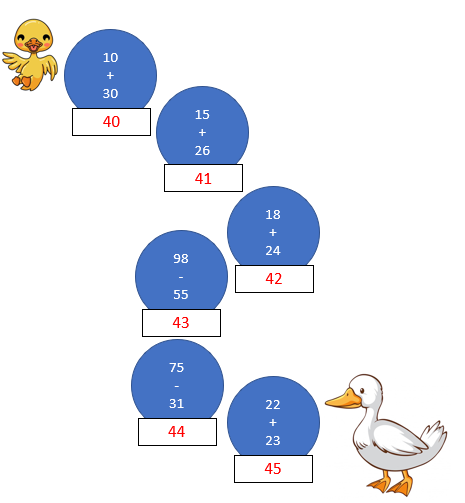
\includegraphics[width=4.84443in,height=5.24031in]{media/image17.png}

Professor(a), se julgar pertinente, chame a atenção dos alunos para o
fato de o patinho pular de um em um passo para alcançar a mamãe pata.

\subsubsection{5}\label{section-12}

paulinho tem uma coleção enorme de figurinhas. ele tem 20 figurinhas de
jogadores de futebol, 15 figurinhas de carros esportivos, 17 figurinhas
de jogos de \emph{vídeo game} e mais 26 figurinhas de seu personagem
preferido. na escola, paulinho perdeu 10 figurinhas jogando tapão. com
quantas figurinhas paulinho ficou no total. \textless{}4
linhas\textgreater{}

Professor(a), aqui temos uma situação problema, em que o aluno precisa
usar a adição e a subtração para obter a resposta. Oriente-os caso
estejam com dificuldade de encontrar a resposta correta, além de ler o
problema com eles, visto que ainda têm dificuldade de leitura e escrita.
Se necessário, distribua palitos para auxiliar os alunos na contagem.
Oriente-os a fazer uma adição por vez, assim como a fazer a subtração
somente no final.

\(15 + 17 + 26 = 58\) \(\rightarrow \ \ 58 - 10 = 48\).

\subsubsection{6}\label{section-13}

Joana tem muita vontade de comprar a boneca sonequinha. ela descobriu
que sua sonhada boneca custa 56 reais. joana abriu seu cofrinho e
percebeu que tem somente 25 reais, porém, lembrou que ganhará mais 15
reais no fim de semana. quantos reais faltam para joana comprar a
boneca? \textless{}4 linhas\textgreater{}

Professo(a), essa atividade tem a mesma proposta da atividade anterior.
Siga a mesma estratégia que tenha funcionado. Não se esqueça de ler o
problema com os alunos, em virtude da dificuldade com leitura e escrita
dessa faixa etária.

\subsubsection{7}\label{section-14}

demonstre várias formas de formarmos o numero 100 através da adição de
duas parcelas.

\begin{longtable}[]{@{}llllllllll@{}}
\toprule
50 & + & & + & & + & & + & & +\tabularnewline
50 & & & & & & & & &\tabularnewline
100 & & 100 & & 100 & & 100 & & 100 &\tabularnewline
\bottomrule
\end{longtable}

\begin{longtable}[]{@{}llllllllll@{}}
\toprule
& + & & + & & + & & + & & +\tabularnewline
& & & & & & & & &\tabularnewline
100 & & 100 & & 100 & & 100 & & 100 &\tabularnewline
\bottomrule
\end{longtable}

Professor(a), aqui temos uma série de resultados possíveis. Faça alguns
exemplos com os alunos e oriente-os a utilizarem números mais simples,
como 10, 20 e etc. Aproveite para lembra-los o conceito de parcelas,
pois, talvez, alguns não saibam ainda o que significa essa palavra.
Podemos aproveitar essa atividade para ampliar o vocabulário dos alunos.

\subsubsection{8}\label{section-15}

demonstre várias formas de formarmos o numero 10 através da subtração de
duas parcelas.

\begin{longtable}[]{@{}llllllllll@{}}
\toprule
100 & + & & + & & + & & + & & +\tabularnewline
90 & & & & & & & & &\tabularnewline
10 & & 10 & & 10 & & 10 & & 10 &\tabularnewline
\bottomrule
\end{longtable}

\begin{longtable}[]{@{}llllllllll@{}}
\toprule
& + & & + & & + & & + & & +\tabularnewline
& & & & & & & & &\tabularnewline
10 & & 10 & & 10 & & 10 & & 10 &\tabularnewline
\bottomrule
\end{longtable}

Professor(a), aqui podemos usar a mesma estratégia da atividade
anterior.

\subsubsection{9}\label{section-16}

resolva o enigma e descubra qual é o número. pinte-o no quadro.

- Sou maior que 5.

- sou menor do que 50.

- uma das minhas parcelas pode ser 12.

- uma das minhas parcelas também pode ser 10.

- se uma das minhas parcelas for 20, a outra não pode ser maior do que
dois.

\begin{longtable}[]{@{}lll@{}}
\toprule
22 & 12 & 10\tabularnewline
32 & 50 & 5\tabularnewline
20 & 2 & 42\tabularnewline
\bottomrule
\end{longtable}

Professor(a), o aluno deve perceber que o número em questão é o 22.

\subsubsection{10}\label{section-17}

Pinte da mesma cor os números que, adicionados, em três parcelas, podem
formar os números que se pedem.

\begin{longtable}[]{@{}lllll@{}}
\toprule
2 & 10 & 5 & & 10\tabularnewline
25 & 3 & 22 & & 50\tabularnewline
28 & 50 & 15 & & 100\tabularnewline
\bottomrule
\end{longtable}

Professor(a), explique aos alunos que só existe uma combinação possível
para cada número. Oriente também a pintarem as parcelas na cor
equivalente aos resultados esperados na coluna do lado direito. Peça
para eles conferirem antes de pintar. As combinações são:

\begin{longtable}[]{@{}lllll@{}}
\toprule
amarelo & verde & amarelo & & \(2 + 3 + 5 = 10\)\tabularnewline
verde & amarelo & azul & & \(25 + 10 + 15 = 50\)\tabularnewline
azul & azul & verde & & \(28 + 50 + 22 = 100\)\tabularnewline
\bottomrule
\end{longtable}

\subsubsection{11}\label{section-18}

patrick quer vender seu album de figurinhas por 56 reais. um amiguinho
quer COMPRA-LO, mas só tem 13 reais. além disso, só podera pagar o resto
em duas vezes, e a primeira parcela tem que ser menor que a primeira.
crie três formas de pagamento para o amigo de patrick.

\begin{longtable}[]{@{}lll@{}}
\toprule
& 56 -- 13 = & 43\tabularnewline
& &\tabularnewline
& menor & maior\tabularnewline
1° formato & 20 & 23\tabularnewline
& menor & maior\tabularnewline
2° formato & &\tabularnewline
& menor & maior\tabularnewline
3° formato & &\tabularnewline
\bottomrule
\end{longtable}

Professor(a), aqui temos uma resolução de situação problema. Oriente os
alunos a primeiro descobrirem quanto falta para o amigo de Patrick pagar
o álbum de figurinhas. Tem uma proposta de resposta orientada que você
pode usar como exemplo, caso julgar necessário.

\subsubsection{12}\label{section-19}

assinale uma forma de agruparmos 45 reais utilizando as seguintes
cédulas.

\textless{}Criar uma figura conforme o modelo a seguir. Se necessário
desconfigure as notas de reais, contanto que as cédulas fictícias tenham
o mesmo valor. Coloque uma bola para que o aluno assinale.

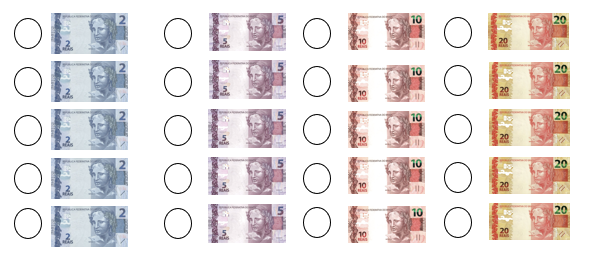
\includegraphics[width=5.90556in,height=2.71667in]{media/image18.png}

Ppfessor(a), nessa atividade também temos várias respostas possíveis. É
importante que o aluno consiga compreender a ideia de composição por
diferentes adições. Peça para que eles criem outra forma além da
encontrada na atividade, e registrem na lousa. Essa atividade é
importante para trabalhar educação financeira. Algumas das combinações
podem ser:

\(20 + 20 + 5,\ \ \ \ 10 + 10 + 10 + 10 + 5\), 2+2+2+2+2+10+20+5 e etc.

\subsubsection{13}\label{section-20}

em uma partida de futebol foram marcados 10 gols. o time a venceu o time
b. identifique os possíveis placares.

\textless{}Inserir uma figura conforme o modelo a seguir.
https://br.freepik.com/vetores-gratis/conjunto-de-simbolos-ou-emblemas-de-escudo-de-nove\_8998384.htm\#query=escudo\%20de\%20time\&position=5\&from\_view=search\&track=ais.\textgreater{}

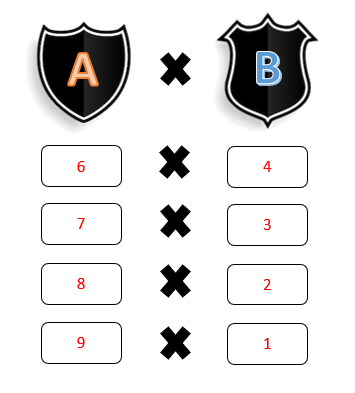
\includegraphics[width=2.78474in,height=3.08282in]{media/image19.png}

Professor(a), oriente os alunos sobre o fato de termos exatamente 4
resultados possíveis.

\subsubsection{14}\label{section-21}

a mãe de reinaldo vai chamar 50 pessoas para sua festa de aniversário.
mas reinaldo tem 10 tios, 8 tias, 15 primos, 9 amiguinhos e 4 vizinhos.

\begin{enumerate}
\def\labelenumi{\Alph{enumi})}
\item
  nesse caso, podemos acrescentar convidados, ou precisamos retirar
  convidados da lista? \textless{}1 linha\textgreater{}
\end{enumerate}

Professor(a), oriente aos alunos a adicionarem a quantidade de
convidados previstos, para descobrirem que esse número é menor do que
50, logo, podem acrescentar convidados. \(10 + 8 + 15 + 9 + 4 = 46.\)

\begin{enumerate}
\def\labelenumi{\Alph{enumi})}
\item
  quantos convidados podemos acrescentar ou quantos convidados
  precisamos retirar? \textless{}1 linha\textgreater{}
\end{enumerate}

\(50 - 46 = 4,\ \)logo podemos acrescentar 4 convidados.

\subsubsection{15}\label{section-22}

analise as caixas com as figuras geométricas. precisamos organizar as
figuras para que cada caixa tenha a mesma quantidade de figuras. sabemos
que temos 16 círculos, 16 quadrados e 16 triângulos, logo, em cada caixa
devem ter 4 quadrados, 4 triângulos e 4 círculos.

\textless{}Inserir uma figura com quatro caixas, identificadas por
letras, contendo círculos, quadrados e triângulos, espalhados de forma
aleatória, conforme o modelo a seguir.

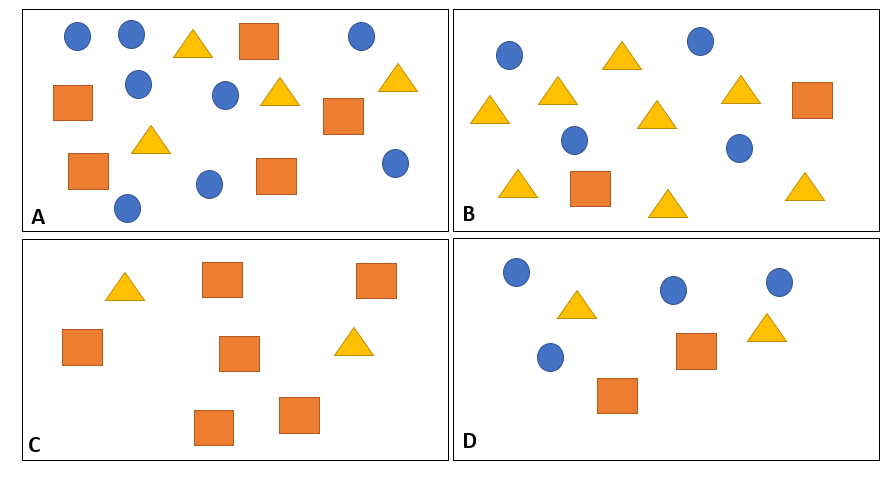
\includegraphics[width=5.90556in,height=3.22917in]{media/image20.png}

\begin{enumerate}
\def\labelenumi{\Alph{enumi})}
\item
  quantos círculos temos que tirar da caixa \textbf{A}? \textless{}1
  linha\textgreater{}
\end{enumerate}

\begin{enumerate}
\def\labelenumi{\arabic{enumi}.}
\setcounter{enumi}{3}
\item
  círculos.
\end{enumerate}

\begin{enumerate}
\def\labelenumi{\Alph{enumi})}
\item
  quantos triângulos temos que tirar da caixa \textbf{B}? \textless{}1
  linha\textgreater{}
\end{enumerate}

4 triângulos.

\begin{enumerate}
\def\labelenumi{\Alph{enumi})}
\item
  Quantos triângulos temos que acrescentar às caixas \textbf{C} e
  \textbf{D}? \textless{}1 linha\textgreater{}
\end{enumerate}

2 triângulos em cada uma.

\begin{enumerate}
\def\labelenumi{\Alph{enumi})}
\item
  quantos quadrados temos que tirar da caixa \textbf{A}? \textless{}1
  linha\textgreater{}
\end{enumerate}

1 quadrado.

\begin{enumerate}
\def\labelenumi{\Alph{enumi})}
\item
  quantos quadrados temos que tirar da caixa \textbf{C}? \textless{}1
  linha\textgreater{}
\end{enumerate}

2 quadrados.

\begin{enumerate}
\def\labelenumi{\Alph{enumi})}
\item
  quantos quadrados temos que acrescentar às caixas \textbf{B} e
  \textbf{D}? \textless{}1 linha\textgreater{}
\end{enumerate}

2 quadrados em cada caixa.

\begin{enumerate}
\def\labelenumi{\Alph{enumi})}
\item
  se juntarmos todas as figuras em uma única caixa, com quantas figuras
  essa caixa fica?
\end{enumerate}

\(16 + 16 + 16 + 16 = 64\ \) figuras.

Professor(a), o mais importante nessa atividade é ressaltar com as
crianças os conceitos de retirar, acrescentar e juntar.

\subsection{TREINO}\label{treino-1}

\subsubsection{01}\label{section-23}

benício e bernardo são irmãos. um dia eles resolveram juntar todas as
suas figurinhas. benício tem 25 e bernardo tem 32. quantas figurinhas os
irmãos têm juntos?

\begin{enumerate}
\def\labelenumi{\Alph{enumi})}
\item
  7
\item
  25
\item
  32
\item
  57
\end{enumerate}

SAEB: 2N1.7 Calcular o resultado de adições e subtrações, envolvendo
número naturais de até 3 ordens.

BNCC: (EF01MA08) Resolver e elaborar problemas de adição e de subtração,
envolvendo números de

até dois algarismos, com os significados de juntar, acrescentar, separar
e retirar, com o suporte

de imagens e/ou material manipulável, utilizando estratégias e formas de
registro pessoais.

\begin{enumerate}
\def\labelenumi{\alph{enumi})}
\item
  Incorreta. O aluno pode ter subtraído ao invés de adicionar.
\item
  Incorreta. O aluno considerou somente as figurinhas de Benício.
\item
  Incorreta. O aluno considerou somente as figurinhas de Bernardo.
\item
  Correta. O aluno somou as figurinhas encontrando 25 + 32 = 57.
\end{enumerate}

\subsubsection{02}\label{section-24}

o primeiro ano do colégio se dividiu em dois times para jogar basquete.
foi meninos contra meninas. os dois times fizeram 30 cestas ao todo. as
meninas venceram os meninos. identifique qual o único resultado
possível.

\begin{enumerate}
\def\labelenumi{\Alph{enumi})}
\item
  meninas 16 x meninos 15.
\item
  meninas 16 x Meninos 14.
\item
  meninas 15 x meninos 14.
\item
  meninas 15 x meninos 13.
\end{enumerate}

SAEB: 2N1.8 - Compor ou decompor números naturais de até 3 ordens por
meio de diferentes adições.

BNCC: (EF01MA07) Compor e decompor número de até duas ordens, por meio
de diferentes adições, com o suporte de material manipulável,
contribuindo para a compreensão de características do sistema de
numeração decimal e o desenvolvimento de estratégias de cálculo.

\begin{enumerate}
\def\labelenumi{\alph{enumi})}
\item
  Incorreta. Adicionando 16 a 15 compomos um número maior do que 30.
\item
  Correta. Adicionando 16 a 14 compomos a exata quantidade de cestas do
  jogo, ou seja, 30.
\item
  Incorreta. Adicionando 15 a 14 compomos um número igual a 29,
  portanto, menos do que 30.
\item
  Incorreta. Adicionando 15 a 13 compomos um número igual a 28,
  portanto, também menor do que 30.
\end{enumerate}

\subsubsection{03}\label{section-25}

vinícius quer comprar um lanche e só tem 15 reais. pediu para sua mãe e
ela lhe deu mais 12 reais. pediu mais dinheiro ainda para a sua vó e ela
lhe deu mais 10 reais. vinicius percebeu que daria para comprar, além do
lanche, um sorvete de cinco reais. qual o preço do lanche?

\begin{enumerate}
\def\labelenumi{\Alph{enumi})}
\item
  15
\item
  32
\item
  37
\item
  42
\end{enumerate}

SAEB: 2N2.1 -- Resolver problemas de adição ou de subtração, envolvendo
números naturais de até 3 ordens, com os significados de juntar,
acrescentar, separar ou retirar.

BNCC: (EF01MA08) Resolver e elaborar problemas de adição e de subtração,
envolvendo números de até dois algarismos, com os significados de
juntar, acrescentar, separar e retirar, com o suporte de imagens e/ou
material manipulável, utilizando estratégias e formas de registro
pessoais.

\begin{enumerate}
\def\labelenumi{\alph{enumi})}
\item
  Incorreta. O aluno pode ter confundido o valor do lanche com o valor
  que Vinícius tinha.
\item
  Correta. O aluno acrescentou o valor do dinheiro que Vinícius tinha
  aos valores que ganhou, depois, retirou o valor do sorvete para
  descobrir o valor do lanche, logo, \(15 + 12 + 10 - 5 = 32\).
\item
  Incorreta. O aluno pode ter esquecido de retirar o valor do sorvete.
\item
  Incorreta. O aluno acrescentou o valor do sorvete ao invés de retirar.
\end{enumerate}

\subsubsection{\texorpdfstring{\\
}{ }}\label{section-26}

\section{MÓDULO 3: MAMÃE, ESTOU
CRESCENDO!}\label{muxf3dulo-3-mamuxe3e-estou-crescendo}

Professor(a), nesse módulo vamos desenvolver as habilidades concernentes
aos conceitos de massa, volume e comprimento. Desenvolver nos alunos a
ideia da necessidade de criarmos padrões de comparação para que medidas
sejam feitas com cada vez mais precisão.

Habilidades da SAEB:

\begin{itemize}
\item
  Comparar comprimentos, capacidades ou massas ou ordenar imagens de
  objetos com base na comparação visual de seus comprimentos,
  capacidades ou massas.
\item
  Estimar/inferir medida de comprimento, capacidade ou massa de objetos,
  utilizando unidades de medida convencionais ou não ou medir
  comprimento, capacidade ou massa de objetos.
\item
  Identificar a medida de comprimento, da capacidade ou da massa de
  objetos, dada a imagem de um instrumento de medida.
\item
  Reconhecer unidades de medida e/ou instrumentos utilizados para medir
  comprimento, tempo, massa ou capacidade.
\end{itemize}

\subsection{CONTEÚDO}\label{conteuxfado-2}

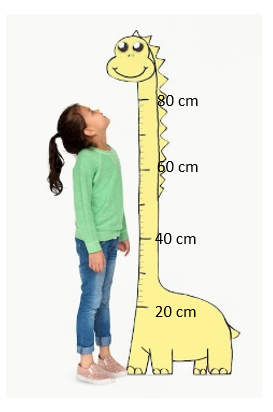
\includegraphics[width=1.67708in,height=2.53098in]{media/image21.png}

\begin{quote}
você sabe qual é a sua altura? você sabe qual é a sua massa? eu tenho
massa? mas não é bolo que tem massa? se tenho massa, como faço pra
medir?

mariana é uma menina muito esperta, que cresce de forma saudável a cada
ano. sua mamãe colou uma medidor na parede de seu quarto, e a cada ano
elas anotam a altura de mariana juntas.
\end{quote}

\textless{}https://br.freepik.com/fotos-premium/escala-crescente-da-altura-alta-da-medida-da-crianca\_3375107.htm\#query=altura\%20de\%20crian\%C3\%A7a\&position=25\&from\_view=search\&track=ais.
Favor colocar as cotas de altura.\textgreater{}

Mariana está agora com 80 cm, que é a altura de uma mesa de escritório.
além disso, a mamãe de mariana também comprou uma balança para medir seu
peso, que na verdade é a sua massa. observe:

\textless{}https://br.freepik.com/vetores-premium/ilustracao-em-escala-industrial-em-fundo-transparente\_23844742.htm\#query=balan\%C3\%A7a\%20digital\&position=37\&from\_view=search\&track=ais.
Colocar o peso de Mariana em 18 kg.\textgreater{}

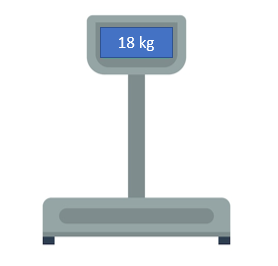
\includegraphics[width=2.13542in,height=2.04324in]{media/image22.png}

mariana está agora com 18 kg, que é a massa de uma poltrona da sala. mas
se a poltrona da sala e a mariana tem a mesma massa, porque a poltrona é
tão maior que mariana? cada corpo tem uma capacidade diferente de ocupar
espaço. essa capacidade é o que chamamos de volume. para medirmos
comprimento usamos a unidade metros, para medirmos massa usamos a medida
quilograma, e para medirmos o espaço ocupado, ou seja, o volume, usamos
a medida litros. os líquidos por exemplo são medidos pelo volume em
litros, como nos refrigerantes e sucos.

\subsection{ATIVIDADES }\label{atividades-2}

\subsubsection{01}\label{section-27}

cricule de azul o que compramos por quilograma (kg), de verde o que
compramos por litros (L) e de vermelho o que compramos por unidades.

\textless{}
https://br.freepik.com/vetores-premium/compra-de-mantimentos-frescos\_19552867.htm\#query=market\%20products\&position=9\&from\_view=search\&track=ais

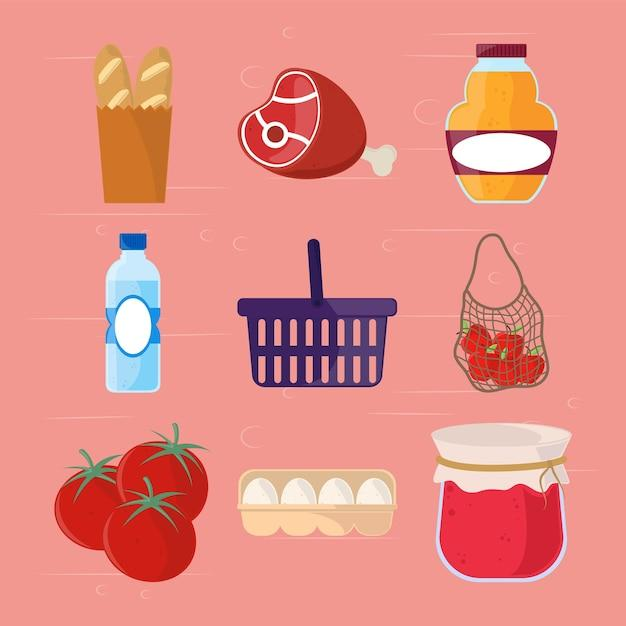
\includegraphics[width=3.53125in,height=3.53125in]{media/image23.jpg}

Professor(a), oriente os alunos a lembrarem das vezes que foram ao
supermercado com os pais. Corrija a atividade com eles, mas permita que
eles tentem fazer sozinhos. Alguns dos itens são pedidos por unidades,
porém são pagos pela unidade de medidas, como é o caso dos pães. Se eles
responderem unidade, não impute como erro, mas ressignifique, explicando
que para o pagamento ser justo, é necessário que a cobrança seja feita
pelo quilograma ou litro. Assim os alunos começam a perceber a real
importância das unidades de medidas. Outra coisa importante, que pode
acontecer, é alguns alunos circularem a geleias como litros. Explique
que somente líquidos são medidos assim, e que massas pastosas são
medidas em quilogramas.

\subsubsection{02}\label{section-28}

Circule os itens que podem ser medidos em metros.

\textless{}Crie a figura conforme o modelo, utilizando as referências:
https://br.freepik.com/vetores-premium/mesa-de-madeira\_31804490.htm\#query=mesa\%20desenho\&position=5\&from\_view=search\&track=ais;
https://br.freepik.com/vetores-gratis/adesivo-de-pacote-de-saco-de-acucar-em-fundo-branco\_18055550.htm\#query=a\%C3\%A7ucar\%20desenho\&position=2\&from\_view=search\&track=ais
(traduzir -- açúcar);
https://br.freepik.com/vetores-gratis/fatia-de-queijo-saboroso\_3077481.htm\#query=queijo\%20desenho\&position=7\&from\_view=search\&track=ais;
https://br.freepik.com/vetores-gratis/beber\_23715247.htm\#query=refri\%20desenho\&position=9\&from\_view=search\&track=ais;
https://br.freepik.com/vetores-gratis/desenho-de-adesivo-com-rolo-de-corda-isolado\_18184169.htm\#query=cordadesenho\&position=0\&from\_view=search\&track=ais;
\href{https://br.freepik.com/vetores-premium/oleo-de-motor-de-substituicao-mecanico-de-automoveis-segurando-uma-lata-de-oleo-de-motor-isolado-no-fundo-branco-manutencao-do-servico-da-estacao-motor-e-mecanismos-de-lubrificacao-design-plano-de-ilustracao-vetorial_23005619.htm\#query=gasolina\%20gal\%C3\%A3odesenho\&position=6\&from_view=search\&track=ais}{\emph{https://br.freepik.com/vetores-premium/oleo-de-motor-de-substituicao-mecanico-de-automoveis-segurando-uma-lata-de-oleo-de-motor-isolado-no-fundo-branco-manutencao-do-servico-da-estacao-motor-e-mecanismos-de-lubrificacao-design-plano-de-ilustracao-vetorial\_23005619.htm\#query=gasolina\%20gal\%C3\%A3odesenho\&position=6\&from\_view=search\&track=ais}}.\textgreater{}

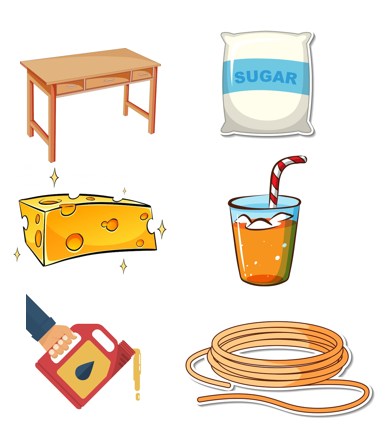
\includegraphics[width=4.02139in,height=4.59439in]{media/image24.png}

Professor(a), é importante que o aluno perceba que somente a mesa e a
corda podem ser medidas através do metro.

\subsubsection{03}\label{section-29}

Ligue os produtos à unidade mais adequada.

\textless{}Inserir quadro conforme o modelo a seguir.\textgreater{}

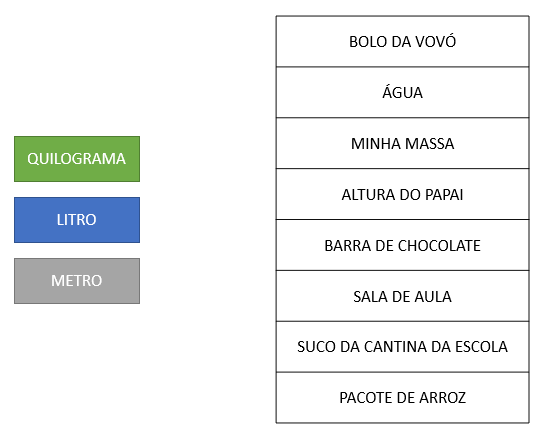
\includegraphics[width=4.86920in,height=3.96016in]{media/image25.png}

\subsubsection{04}\label{section-30}

DESENHE NOS QUADROS ABAIXO, ALGO QUE POSSA SER MEDIDO ATRAVÉS DESSES
INSTRUMENTOS.

\textless{} insira os quadros e as figuras, conforme o modelo a seguir,
utilizando as referências:
https://br.freepik.com/vetores-premium/bonito-governante-engracado-acenando-o-personagem-de-mao\_23415941.htm\#page=3\&query=UMA\%20R\%C3\%89GUA\%20DESENHO\&position=39\&from\_view=search\&track=ais;
https://br.freepik.com/vetores-gratis/balanca-digital-em-fundo-branco\_16262850.htm\#query=BALAN\%C3\%87A\%20DESENHO\&position=3\&from\_view=search\&track=ais;
https://br.freepik.com/vetores-gratis/adesivo-de-copo-de-medicao-em-fundo-branco\_18180135.htm\#query=COPO\%20MEDIDORDESENHO\&position=2\&from\_view=search\&track=ais;
https://br.freepik.com/vetores-premium/fita-metrica-para-medir-a-distancia-em-centimetros-e-milimetros-rabiscar-a-coloracao-linear-dos-desenhos-animados\_30247681.htm\#query=TRENA\%20DESENHO\&position=45\&from\_view=search\&track=ais.\textgreater{}

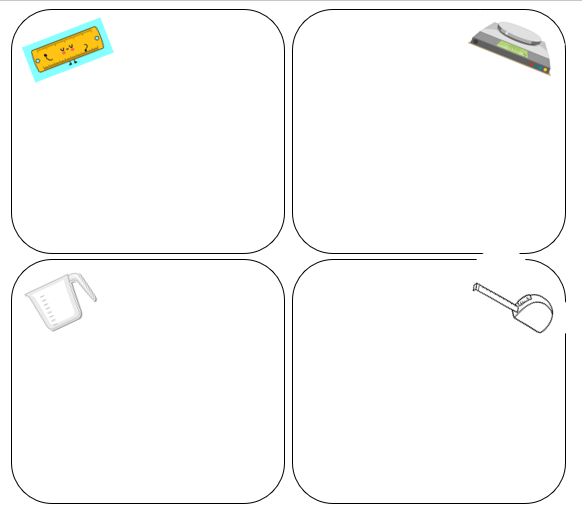
\includegraphics[width=6.43650in,height=5.62891in]{media/image26.png}

Professor(a), oriente os alunos, caso não entendam os desenhos.
Principalmente o da trena, pois talvez algumas crianças nunca tenham
visto uma, além do copo medidor. Deixe que a imaginação deles flua. Pelo
desenho será possível identificar se estão absorvendo o conceito de
medição.

\subsubsection{05}\label{section-31}

Ligue as pessoas às suas camas.

\textless{}Crie um quadro conforme o modelo a seguir, utilizando as
referências:
https://br.freepik.com/vetores-premium/homem-segurando-binoculos-pessoa-olhando-para-o-horizonte-futuro\_30928646.htm\#query=adulto\%20alto\%20DESENHO\&position=6\&from\_view=search\&track=ais;
https://br.freepik.com/vetores-premium/rapaz-dos-desenhos-animados-com-guitarra-criancas-tocando-instrumento-musical-em-casa-aula-ou-performance-artista-de-educacao-musical-ou-ferramentas-de-som-publicidade-vector-hobby-carreira-e-ilustracao-de-atividade-de-lazer\_26152103.htm\#query=adulto\%20baixo\%20DESENHO\&position=8\&from\_view=search\&track=ais;
https://br.freepik.com/vetores-gratis/personagem-de-desenho-animado-de-menino-bonito-em-fundo-branco\_28457881.htm\#query=menino\%20DESENHO\&position=5\&from\_view=search\&track=ais;
https://br.freepik.com/vetores-gratis/cama-com-travesseiro-e-lencol-azul\_2204447.htm\#query=cama\%20DESENHO\&position=1\&from\_view=search\&track=ais.\textgreater{}

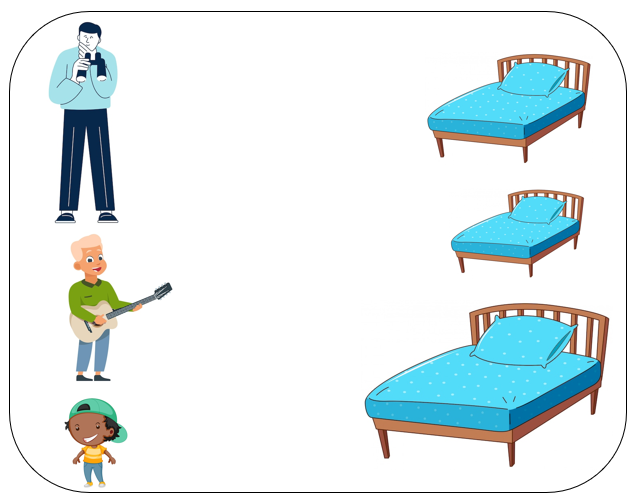
\includegraphics[width=6.28790in,height=4.93257in]{media/image27.png}

Professor(a), é importante que o aluno reconheça que as diferenças de
alturas entre as pessoas se reflete na diferença de tamanho das camas.
Assim o aluno conseguirá inferir medida de comprimento.

\subsubsection{06}\label{section-32}

pinte como a jarra maior ficaria, se colocassemos todo o liquido das
jarras menores nela.

\protect\hypertarget{_heading=h.gjdgxs}{}{}\textless{}Inserir a figura
usando a referência:
https://br.freepik.com/vetores-gratis/adesivo-de-copo-de-medicao-em-fundo-branco\_18180135.htm\#query=COPO\%20MEDIDORDESENHO\&position=2\&from\_view=search\&track=ais.
Colocar as quantidades conforme o modelo a seguir.\textgreater{}

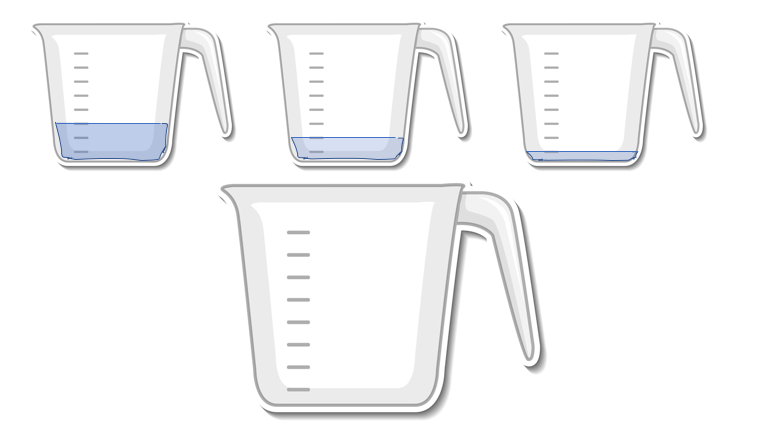
\includegraphics[width=5.90556in,height=3.37222in]{media/image28.png}

Professor(a), é importante desenvolver nos alunos uma capacidade de
medição empírica, uma vez que não temos a unidade presente na jarra.
Oriente os alunos a contarem a quantidade de riscos das jarras. Eles
devem pintar até a sexta marcação.

\subsubsection{07}\label{section-33}

se cada marcação da jarra da atividade anterior medisse meio litro,
quantos litros teriam sido colocados nela? \textless{}1
linha\textgreater{}

Professor(a), podemos aproveitar essa atividade para lembrarmos o
conteúdo do módulo anterior, onde os alunos terão a oportunidade de
lembrar os conceitos de adição, dentro de um contexto de medição.

\subsubsection{08}\label{section-34}

seguindo a mesma ideia da atividade anterior, ou seja, considerando que
cada risquinho mede meio litro, qual é a capacidade total dessa jarra.
\textless{}1 linha\textgreater{}

Professor(a), continuando a linha de raciocínio da atividade anterior,
aqui podemos desenvolver no aluno a habilidade de estimar a capacidade
de um instrumento de medida. O aluno deve chegar a resposta de 4 litros

\subsubsection{09}\label{section-35}

utilize uma régua e estime o comprimento das figuras a seguir.

\textless{}Inserir os quadros com as figuras conforme os modelos a
seguir. Referências na figura.\textgreater{}

\begin{longtable}[]{@{}l@{}}
\toprule
\begin{minipage}[t]{0.97\columnwidth}\raggedright\strut
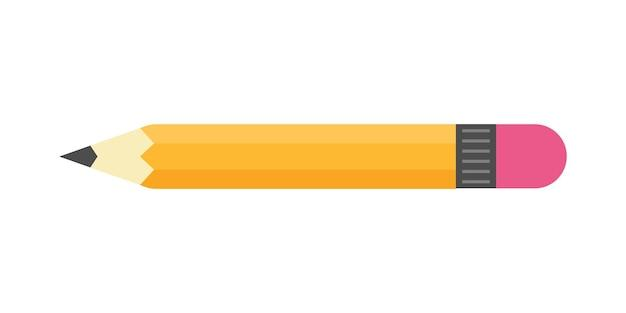
\includegraphics[width=5.91597in,height=0.90625in]{media/image29.jpg}

https://br.freepik.com/vetores-premium/icone-de-lapis-em-estilo-simples-ilustracao-vetorial-de-equipamentos-de-educacao-em-fundo-isolado-conceito-de-negocio-de-sinal-de-ferramenta-de-desenho\_30026502.htm\#query=lapis\&position=6\&from\_view=search\&track=sph\strut
\end{minipage}\tabularnewline
medida:\tabularnewline
\bottomrule
\end{longtable}

\begin{longtable}[]{@{}l@{}}
\toprule
\begin{minipage}[t]{0.97\columnwidth}\raggedright\strut
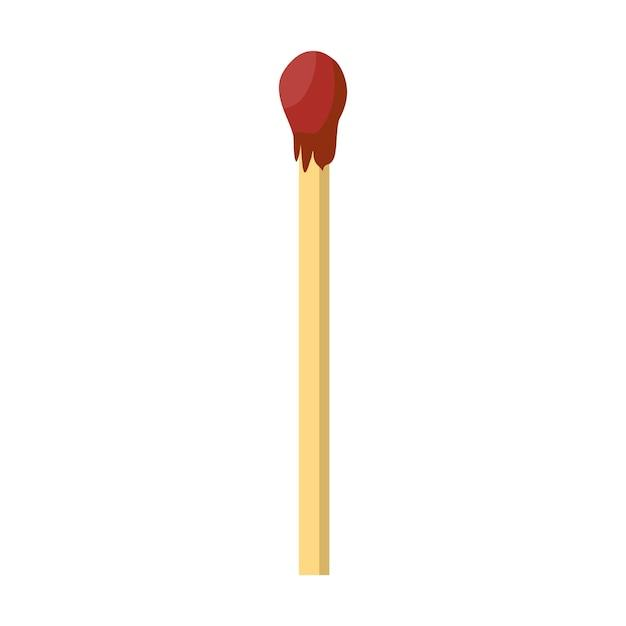
\includegraphics[width=0.69250in,height=4.62743in]{media/image30.jpg}

https://br.freepik.com/vetores-premium/objetos-vetoriais-isolados-de-desenho-animado-combinam-e-fogo\_29291308.htm\#query=palito\%20de\%20f\%C3\%B3sforo\%20desenho\&position=9\&from\_view=search\&track=ais\strut
\end{minipage}\tabularnewline
medida:\tabularnewline
\bottomrule
\end{longtable}

\begin{longtable}[]{@{}l@{}}
\toprule
\begin{minipage}[t]{0.97\columnwidth}\raggedright\strut
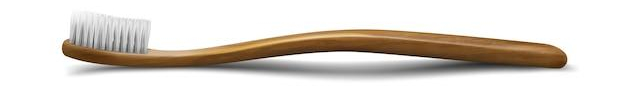
\includegraphics[width=5.90556in,height=0.75000in]{media/image31.jpg}

https://br.freepik.com/vetores-premium/objetos-vetoriais-isolados-de-desenho-animado-combinam-e-fogo\_29291308.htm\#query=palito\%20de\%20f\%C3\%B3sforo\%20desenho\&position=9\&from\_view=search\&track=ais\strut
\end{minipage}\tabularnewline
medida:\tabularnewline
\bottomrule
\end{longtable}

Professor(a), oriente os alunos quanto ao fato de suas réguas medirem
comprimento menores do que um metro. Explique para eles que o centímetro
é uma subdivisão dele. Não é momento de quantificar essa subdivisão.
Basta que entendam que se trata de outra unidade para medir
comprimentos.

\subsection{TREINO}\label{treino-2}

\subsubsection{01}\label{section-36}

informe qual das crianças abaixo é a mais alta?

\textless{}
https://br.freepik.com/vetores-gratis/quatro-criancas\_4906544.htm\#page=2\&query=crian\%C3\%A7as\%20com\%20diferentes\%20alturas\%20desenho\&position=13\&from\_view=search\&track=ais.\textgreater{}

\begin{quote}
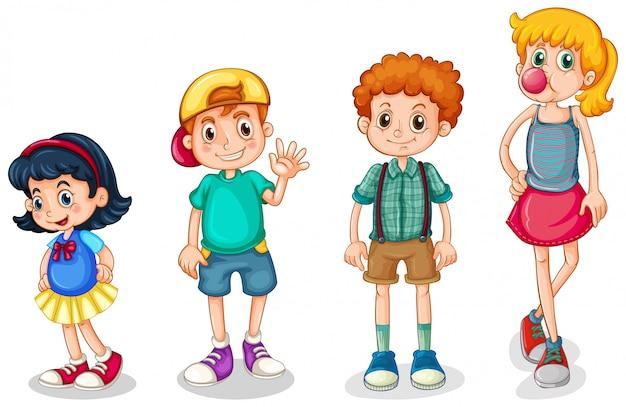
\includegraphics[width=4.23198in,height=2.75148in]{media/image32.jpg}
\end{quote}

A) A menina de saia amarela.

B) a menina mascando goma.

C) O menino de boné.

D) o menino de tênis azul.

SAEB: 2M1.1 - Comparar comprimentos, capacidades ou massas ou ordenar
imagens de objetos com base na comparação visual de seus comprimentos,
capacidades ou massas.

BNCC: (EF01MA15) Comparar comprimentos, capacidades ou massas,
utilizando termos como mais alto, mais baixo, mais comprido, mais curto,
mais grosso, mais fino, mais largo, mais pesado, mais leve, cabe mais,
cabe menos, entre outros, para ordenar objetos de uso cotidiano.

a) Incorreta. A menina de saia amarela é a mais baixa.

b) Correta. A menina mascando goma tem o maior comprimento de altura,
logo é a mais alta.

c) Incorreta. O menino de boné é o terceiro mais alto, ou o segundo mais
baixo.

d) Incorreta. O menino de tênis azul é o segundo mais alto.

\subsubsection{02}\label{section-37}

Qual o melhor instrumento de medida para medirmos o comprimento de uma
mesa?

\begin{quote}
A) balança

B) copo de medir

C) régua

D) panela

SAEB: 2M1.4 - Reconhecer unidades de medida e/ou instrumentos utilizados
para medir comprimento, tempo, massa ou capacidade.

BNCC: (EF01MA15) Comparar comprimentos, capacidades ou massas,
utilizando termos como mais alto, mais baixo, mais comprido, mais curto,
mais grosso, mais fino, mais largo, mais pesado, mais leve, cabe mais,
cabe menos, entre outros, para ordenar objetos de uso cotidiano.

a) Incorreta. A balança é utilizada para medir massas em quilogramas.
\end{quote}

b) Incorreta. O copo de medir é utilizado para medir volume em litros.

c) Correta. A régua pode ser utilizada para medir a superfície de uma
mesa, apesar de ser bem menor.

d) Incorreta. A panela só pode ser utilizada também para medir volume,
uma vez que tem capacidade fixa.

\subsubsection{03}\label{section-38}

A imagem mostra a medição da massa da mãe de juliana no visor da
balança. qual é a massa da mãe de juliana. medida em quilogramas?

\textless{}https://br.freepik.com/fotos-gratis/closeup-de-peso-escalas-conceito-de-excesso-de-peso-e-obesidade\_3219089.htm\#page=5\&query=regua\%20medindo\&position=49\&from\_view=search\&track=ais\textgreater{}

\begin{quote}
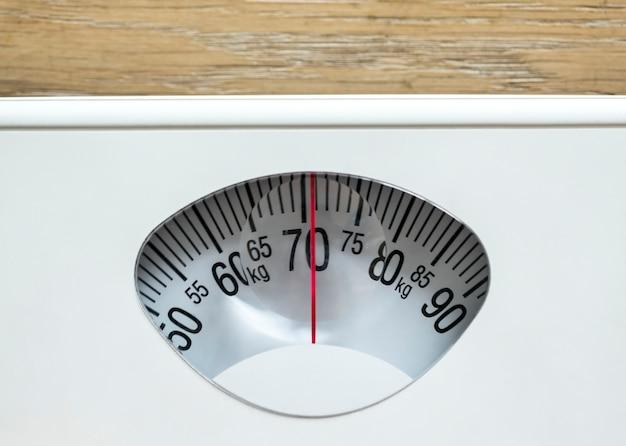
\includegraphics[width=3.03770in,height=1.48580in]{media/image33.jpg}
\end{quote}

A) 69

B) 70

C) 71

D) 72

SAEB: 2M1.3 - Identificar a medida de comprimento, da capacidade ou da
massa de objetos, dada a imagem de um instrumento de medida.

BNCC: (EF01MA15) Comparar comprimentos, capacidades ou massas,
utilizando termos como mais alto, mais baixo, mais comprido, mais curto,
mais grosso, mais fino, mais largo, mais pesado, mais leve, cabe mais,
cabe menos, entre outros, para ordenar objetos de uso cotidiano.

a) Incorreta. O aluno pode ter invertido o sentido de leitura do visor

b) Incorreta. O aluno entendeu que o ponteiro estava sobre o número 70.

c) Correta. O aluno percebeu que o ponteiro está deslocado uma unidade
além do 70.

d) Incorreta. O aluno pensou que cada risquinho valesse 2.

\section{MÓDULO 4: EM QUE DIA VAI CAIR MEU ANIVERSÁRIO?
}\label{muxf3dulo-4-em-que-dia-vai-cair-meu-aniversuxe1rio}

Neste módulo vamos desenvolver nos alunos a habilidade de orientar-se no
tempo, sabendo identificar o tempo presente, assim como prever dias e
horários de eventos futuros.

Habilidades da BNCC: EF01MA16; EF01MA17; EF01MA18.

Habilidades da SAEB:

- Identificar sequência de acontecimentos relativos a um dia.

- Identificar datas, dias da semana ou meses do ano em calendário ou
escrever uma data, apresentando o dia, o mês e o ano.

- Determinar a data de início, a data de término ou a duração de um
acontecimento entre duas datas.

- Determinar o horário de início, o horário de término ou a duração de
um acontecimento.

\subsection{CONTEÚDO}\label{conteuxfado-3}

Todo mundo fica ansioso para chegar o dia do seu próprio aniversário!
não vemos a hora de ganhar presentes, comer bolo, assoprar a velinha e
brincar com os amigos. mas você sabe que dia isso acontecerá? em que dia
da semana? você sabe dizer a que horas vai começar e terminar a sua
festinha?

\textless{}https://br.freepik.com/vetores-premium/personagens-de-desenhos-animados-comemorando-a-festa-de-aniversario\_28760759.htm\#query=festa\%20de\%20aniversario\%20crian\%C3\%A7as\&position=10\&from\_view=search\&track=ais\textgreater{}

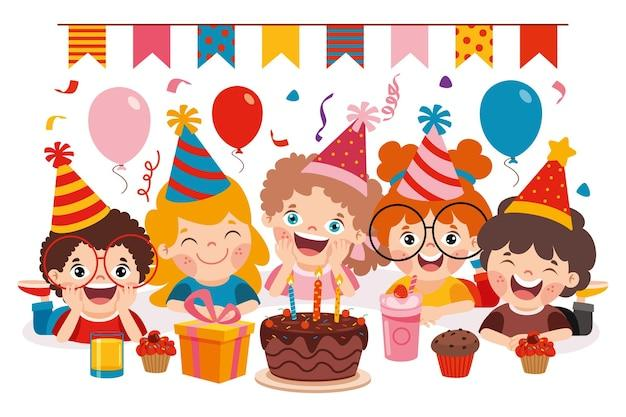
\includegraphics[width=4.02731in,height=2.68282in]{media/image34.jpg}

Vamos lembrar como é organizado nosso calendário?

o ano é dividido em 365 dias de 24 horas cada um. além disso, o ano
também é dividido em 12 meses. você lembra o nome deles e a quantidade
de dias de cada um? observe:

\begin{longtable}[]{@{}llllll@{}}
\toprule
Janeiro & Fevereiro & Março & abril & maio & junho\tabularnewline
31 dias & 28 dias & 31 dias & 30 dias & 31 dias & 30 dias\tabularnewline
Julho & agosto & setembro & outubro & novembro & dezembro\tabularnewline
31 dias & 31 dias & 30 dias & 31 dias & 30 dias & 31 dias\tabularnewline
\bottomrule
\end{longtable}

temos também as semanas que são divididas em 7 dias. observe os nomes
desses dias:

\begin{longtable}[]{@{}lllllll@{}}
\toprule
domingo & 2° feira & 3°feira & 4°feira & 5° feira & 6°feira &
sábado\tabularnewline
\bottomrule
\end{longtable}

\subsection{ATIVIDADES}\label{atividades-3}

\subsubsection{01}\label{section-39}

vamos descobrir que dia é hoje? escreva o que se pede nos quadrados:

\begin{longtable}[]{@{}ll@{}}
\toprule
em que ano estamos? &\tabularnewline
em que mês estamos? &\tabularnewline
que dia do mês é hoje? &\tabularnewline
que dia da semana é hoje? &\tabularnewline
a que horas você fez essa atividade? & : :\tabularnewline
\bottomrule
\end{longtable}

Professor(a), o mais importante nessa atividade é fazer com que o aluno
consiga diferenciar cada classificação do tempo. Saber diferenciar dia
do mês e dia da semana, por exemplo. Oriente-os a preencherem o horário
com horas, minutos e segundos. Essa atividade pode e deve ser usada com
fins de avaliação diagnóstica.

\subsubsection{02}\label{section-40}

pinte os quadrados com a cor equivalente.

\begin{longtable}[]{@{}lllll@{}}
\toprule
Domingo & 30 & Março & 2022 & 13:15:00\tabularnewline
mês & ano & horário & dia do mês & dia da semana\tabularnewline
\bottomrule
\end{longtable}

Professor(a), essa atividade segue a mesma lógica da atividade anterior.
A sequencia de cores é: amarelo, vermelho, laranja, verde e azul

\subsubsection{03}\label{section-41}

pinte no calendário as datas pedidas com a mesma cor.

\begin{longtable}[]{@{}l@{}}
\toprule
meu aniversário\tabularnewline
aniversário da mamãe\tabularnewline
aniversário da vovó\tabularnewline
Aniversário do papai\tabularnewline
\bottomrule
\end{longtable}

\textless{}
https://br.freepik.com/vetores-premium/calendario-de-cores-para-2023-com-um-coelho-de-personagem-fofo-a-semana-comeca-no-domingo-diversao-e-estilo-de-desenho-animado-de-design-brilhante\_34560382.htm\#query=calend\%C3\%A1rio\%20infantil\%202023\%20em\%20portugu\%C3\%AAs\&position=6\&from\_view=search\&track=ais.
Traduzir os nomes dos meses, além das iniciais dos dias da
semana.\textgreater{}

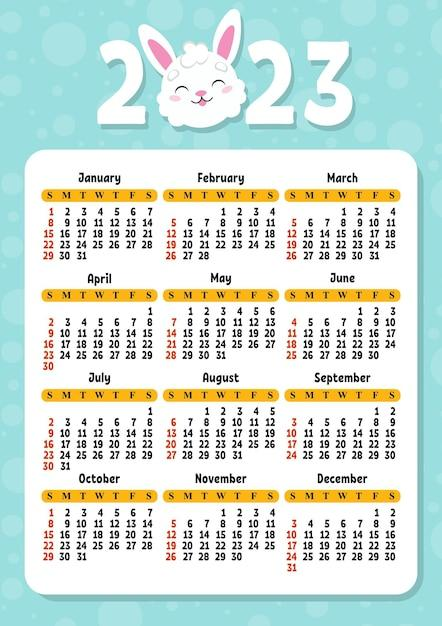
\includegraphics[width=4.71050in,height=6.67143in]{media/image35.jpg}

Professor(a), se o aluno não lembrar essas datas, permita que ele
pergunte a família, adiando a atividade para o dia posterior. Você pode
determinar que o faça como tarefa de casa. Tome um certo cuidado, caso a
criança tenha perdido algum desses parentes, ou então para o caso de ter
duas mães, ou dois pais. Peça para eles desenharem um quadradinho na
data e pintá-lo.

\subsubsection{04}\label{section-42}

analise as figuras e liste a ordem desses acontecimentos em um dia.

\textless{}Inserir as figuras na ordem do modelo a seguir. Utilizar as
referências:
https://br.freepik.com/vetores-premium/garoto-bonito-comendo-delicioso-arroz-frito\_35549113.htm\#query=crian\%C3\%A7a\%20almo\%C3\%A7ando\&position=48\&from\_view=search\&track=ais;
https://br.freepik.com/vetores-gratis/menino-dormir-cama\_4388324.htm\#query=crian\%C3\%A7a\%20acordando\&position=21\&from\_view=search\&track=ais;
https://br.freepik.com/vetores-gratis/menino-que-dorme-na-cama\_1021842.htm\#query=crian\%C3\%A7a\%20acordando\&position=23\&from\_view=search\&track=ais;
https://br.freepik.com/vetores-gratis/uma-garota-fazendo-o-exame\_2607446.htm\#query=crian\%C3\%A7a\%20estudasndo\&position=0\&from\_view=search\&track=ais
e
https://br.freepik.com/vetores-gratis/criancas-felizes-brincando-com-brinquedos\_11575551.htm\#query=crian\%C3\%A7a\%20brincando\&position=32\&from\_view=search\&track=ais
\textgreater{}

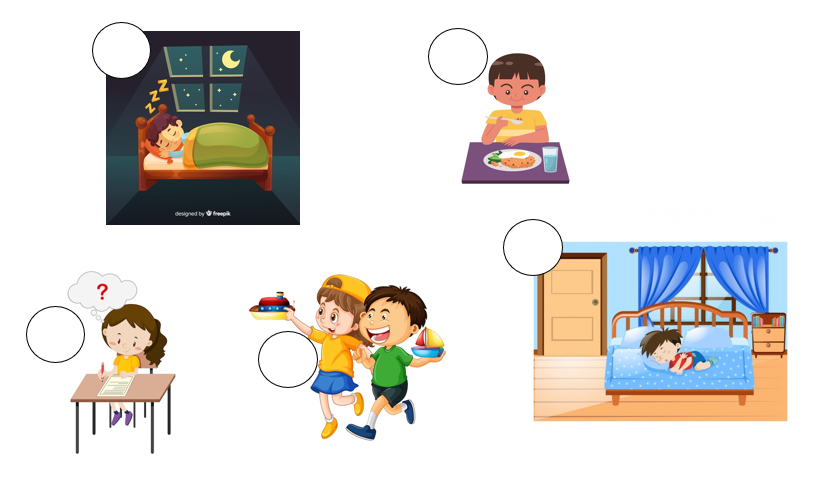
\includegraphics[width=5.90556in,height=3.46597in]{media/image36.png}

Professor(a), os alunos devem seguir a ordem dos acontecimentos
baseando-se em suas rotinas. É importante aqui frisar a importância de
se alimentar no horário certo, trabalhando assim a TCT-Saúde, além de
ressaltar a importância de priorizar o momento dos estudos, ou seja,
estudar antes de brincar. Essa atividade pode ser utilizada também para
os alunos lembrarem a utilização dos números para ordenar coisas.
Oriente-os a utilizarem os números de forma ordinal: 1°, 2° e assim por
diante.

\subsubsection{05}\label{section-43}

Complete oS QUADRADINOS EM BRANCO DO calendário abaixo.

\begin{longtable}[]{@{}l@{}}
\toprule
JANEIRO 2023\tabularnewline
Dom\tabularnewline
1\tabularnewline
8\tabularnewline
15\tabularnewline
22\tabularnewline
29\tabularnewline
\bottomrule
\end{longtable}

Professor(a), oriente os alunos a preencherem os quadrados faltantes dos
dias do mês, assim como os dias da semana.

\subsubsection{06}\label{section-44}

baseado no calendário da atividade anterior, responda.

\begin{enumerate}
\def\labelenumi{\Alph{enumi})}
\item
  que dia da semana é dia 18 de fevereiro?
\end{enumerate}

\textless{}1linha\textgreater{}

4° feira

\begin{enumerate}
\def\labelenumi{\Alph{enumi})}
\item
  quantos sábados temos em janeiro de 2023?
\end{enumerate}

\textless{}1linha\textgreater{}

4 sábados.

\begin{enumerate}
\def\labelenumi{\Alph{enumi})}
\item
  em que dia da semana começa esse mês de janeiro?
\end{enumerate}

\textless{}1linha\textgreater{}

Domingo

\begin{enumerate}
\def\labelenumi{\Alph{enumi})}
\item
  em que dia da semana termina esse mês de janeiro?
\end{enumerate}

\textless{}1linha\textgreater{}

3° feira

\begin{enumerate}
\def\labelenumi{\Alph{enumi})}
\item
  quantos domingos temos nesse mês de janeiro?
\end{enumerate}

\textless{}1linha\textgreater{}

5 Domingos. Professor(a), aproveite para demonstrar que em alguns meses
podemos algum dia da semana se repetindo 5 vezes, ou seja, que o fato de
termos 4 semanas em um mês não significa que teremos sempre 4 repetições
de cada dia da semana. Essa atividade é importante para desenvolver no
aluno a habilidade de ler o calendário com entendimento.

\subsubsection{07}\label{section-45}

Analise o bloco de notas de marcela e responda quantos dias ela esperará
pela resposta que precisa.

\textless{}Inserir a figura da referência:
https://br.freepik.com/vetores-premium/caderno-e-lapis-em-fundo-branco\_10079541.htm\#query=bloco\%20de\%20anota\%C3\%A7\%C3\%B5es\&position=10\&from\_view=search\&track=ais,
incluindo o texto conforme o modelo:\textgreater{}

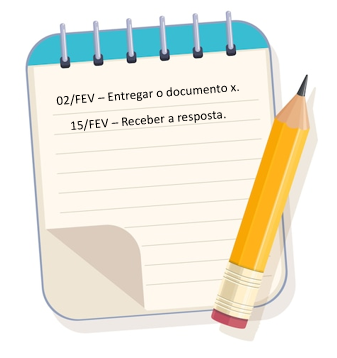
\includegraphics[width=3.51091in,height=3.72969in]{media/image37.png}

Professor(a), é importante que o aluno perceba que entre os dias 02 e 15
de fevereiro se passam 13 dias.

\subsubsection{08}\label{section-46}

Se o dia da semana em que marcela entregou o documento x fosse
sexta-feira, que dia da semana seria o dia da resposta?

\textless{}1 linha\textgreater{}

Professor(a), o dia seria 5° feira. Permita que os alunos criem suas
estratégias inicialmente. Caso não consigam, auxilie-os a contarem os
dias.

\subsubsection{09}\label{section-47}

uma competição de futebol de salão da escola durou uma semana de 7 dias.
a competição começou no dia 10 de outubro de 2021 em um sábado. em que
data terminou o campeonato?

\begin{longtable}[]{@{}ll@{}}
\toprule
ano: & 2021\tabularnewline
mês: & Outubro\tabularnewline
dia do mês: & 16\tabularnewline
dia da semana: & Sexta-feira\tabularnewline
\bottomrule
\end{longtable}

Professor(a), é importante que o aluno perceba que uma semana a partir
de outubro não é suficiente para que o ano ou o mês mudem. Oriente-os a
contarem o primeiro dia.

\subsubsection{10}\label{section-48}

analise os relógios digitais da imagem abaixo e responda:

\textless{}Inserir a figura da referência:
https://br.freepik.com/vetores-premium/um-conjunto-de-relogios-digitais-numeros-eletronicos-ilustracao-vetorial\_32708528.htm\#query=rel\%C3\%B3gio\%20digital\&position=16\&from\_view=search\&track=ais,
inserindo as identificações dos relógios, conforme o modelo a
seguir.\textgreater{}

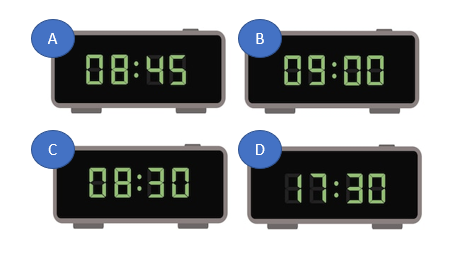
\includegraphics[width=4.34174in,height=2.58209in]{media/image38.png}

\begin{enumerate}
\def\labelenumi{\Alph{enumi})}
\item
  quantas horas se passaram entre o relógio A e B?
\end{enumerate}

\textless{}1linha\textgreater{}

1:45:00

\begin{enumerate}
\def\labelenumi{\Alph{enumi})}
\item
  Quantas horas se passaram entre o relógio c e A?
\end{enumerate}

\textless{}1 linha\textgreater{}

15 minutos

\begin{enumerate}
\def\labelenumi{\Alph{enumi})}
\item
  quantas horas se passaram entre os relógios b e d?
\end{enumerate}

\textless{}1 linha\textgreater{}

8:30:00

\begin{enumerate}
\def\labelenumi{\Alph{enumi})}
\item
  Quantas horas se passaram entre os relógios C e D?
\end{enumerate}

\textless{}1 linha\textgreater{}

9:00:00

Professor(a), oriente os alunos a responderem essa atividade no formato
hh:mm:ss.

\subsubsection{11}\label{section-49}

Mariano olhou para seu celular quando acordou e viu a saeguinte imagem:

\textless{}https://br.freepik.com/vetores-gratis/smartphone-de-tela-de-alarme\_2921841.htm\#query=relogio\%20celular\&position=48\&from\_view=search\&track=ais.\textgreater{}

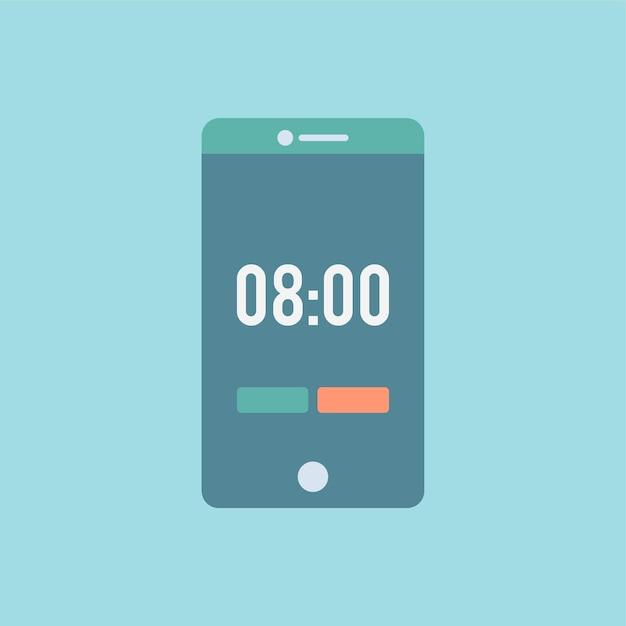
\includegraphics[width=1.70922in,height=2.53170in]{media/image39.jpg}

ele se levantou, se trocou e foi para o trabalho. ele começou a
trabalhar 1 hora e 35 minutos depois. que horas ele começou a trabalhar?

\textless{}1 linha\textgreater{}

09:35:00.

\subsubsection{12}\label{section-50}

PEDRINHO ACORDOU AS 07:30 DA MANHÃ.

https://br.freepik.com/vetores-gratis/um-menino-dormindo-profundamente\_23807622.htm\#query=PEDRINHO\%20ACORDANDO\&position=5\&from\_view=search\&track=ais.\textgreater{};
https://br.freepik.com/vetores-gratis/menino-de-pijama-segurando-a-escova-de-dentes-e-pasta-de-dente\_27547013.htm\#query=ESCOVAR\%20OS\%20DENTES\&position=32\&from\_view=search\&track=ais
https://br.freepik.com/vetores-gratis/um-menino-feliz-comendo-na-mesa\_18973385.htm\#query=CAF\%C3\%81\%20DA\%20MANH\%C3\%83\%20MENINO\&position=12\&from\_view=search\&track=ais;
https://br.freepik.com/vetores-premium/um-menino-brincando-com-gato-fofo\_29183474.htm\#page=2\&query=BRINCANDO\%20COM\%20O\%20GATO\&position=6\&from\_view=search\&track=ais.
\textgreater{}

\begin{quote}
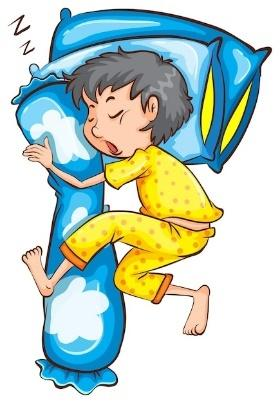
\includegraphics[width=1.27248in,height=1.83120in]{media/image40.jpg}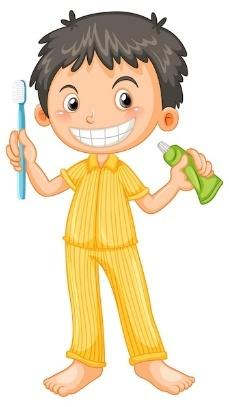
\includegraphics[width=1.04250in,height=1.85399in]{media/image41.jpg}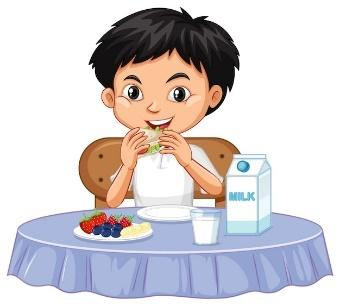
\includegraphics[width=1.54748in,height=1.39171in]{media/image42.jpg}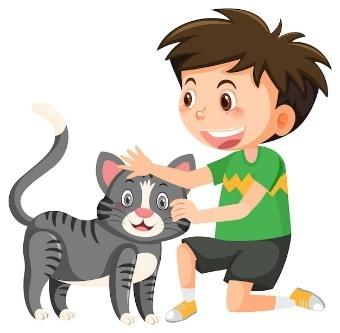
\includegraphics[width=1.54490in,height=1.51274in]{media/image43.jpg}

DEMOROU 15 MINUTOS PARA IR AO BANHEIRO E ESCOVAR OS DENTES. DEPOIS,
DEMOROU MAIS 20 MINUTOS PARA TOMAR O CAFÉ DA MANHÃ. aNTES DE SAIR,
PEDRINHO AINDA FICOU UNS 5 MINUTOS BRINCANDO COM SEU GATINHO.

pinte NO RELÓGIO ABAIXO O HORÁRIO QUE PEDRINHO SAIU PARA IR À ESCOLA.
\end{quote}

\textless{}Inserir uma figura de um relógio, com os números em branco
para o aluno preencher, conforme o modelo a seguir:\textgreater{}


\includegraphics[width=5.90556in,height=1.81944in]{media/image44.png}

Professor(a), oriente o aluno a pintar os quadradinhos e formar o
horário, da mesma forma que aparecem nos relógios digitais. A pintura
deve ficar conforme a figura a seguir:

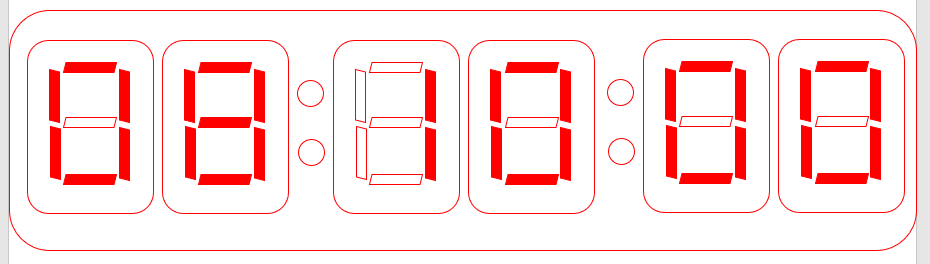
\includegraphics[width=5.90556in,height=1.67639in]{media/image45.png}

\subsection{TREINO}\label{treino-3}

\subsubsection{01}\label{section-51}

Analise o calendário abaixo e indique em qual dia será a última
segunda-feira desse mês.

\begin{longtable}[]{@{}l@{}}
\toprule
fevereiro 2023\tabularnewline
Dom\tabularnewline
\tabularnewline
5\tabularnewline
12\tabularnewline
19\tabularnewline
26\tabularnewline
\bottomrule
\end{longtable}

\begin{quote}
A) 6

B) 26

C) 27

D) 28

SAEB: 2M1.6 - Identificar datas, dias da semana ou meses do ano em
calendário ou escrever uma data, apresentando o dia, o mês e o ano.

BNCC: (EF01MA17) Reconhecer e relacionar períodos do dia, dias da semana
e meses do ano, utilizando calendário, quando necessário.

a) Incorreta. O aluno pode ter confundido com a primeira segunda feira.

b) Incorreta. O aluno pode ter confundido com o Domingo, entendendo que
a 2feira é o primeiro dia a aparecer no calendário.

c) Correta. O aluno buscou a coluna certa e a linha certa.

d) Incorreta. O aluno pode ter confundido a segunda-feira com o ultimo
dia do mês
\end{quote}

\subsubsection{02}\label{section-52}

analise as figuras abaixo e indique qual é a sequência correta de
acontecimentos.

\textless{}https://br.freepik.com/vetores-gratis/antecedentes-da-paisagem-plana-em-tons-roxos\_1001699.htm\#query=anoitecer\&position=2\&from\_view=search\&track=sph;
https://br.freepik.com/vetores-gratis/paisagem-do-por-do-sol-com-lago-nuvens-no-ceu-vermelho-silhuetas-nas-colinas-e-arvores-na-costa\_12407808.htm\#query=amanhecer\&position=1\&from\_view=search\&track=sph

;
https://br.freepik.com/vetores-gratis/paisagem-de-primavera-desenhados-a-mao\_6804642.htm\#query=meio\%20dia\%20paisagem\&position=13\&from\_view=search\&track=ais

;
https://br.freepik.com/vetores-gratis/lua-cheia-noite-oceano-cartoon-ilustracao\_6690817.htm\#query=noite\%20paisagem\&position=10\&from\_view=search\&track=ais

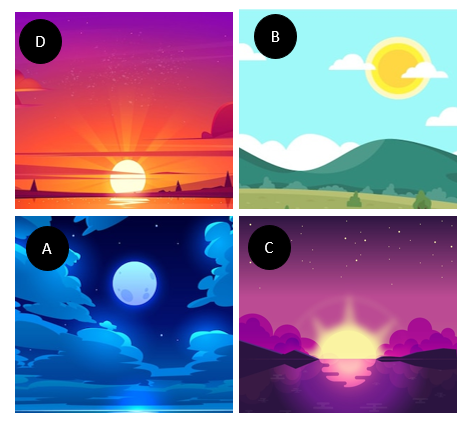
\includegraphics[width=4.85484in,height=4.39645in]{media/image46.png}

\begin{quote}
A) A, B, C, D.

B) B, A, C, D.

C) C, B, A, D.

D) D, B, C, A.

SAEB: 2M1.5 - Identificar sequência de acontecimentos relativos a um dia

BNCC: (EF01MA16) Relatar em linguagem verbal ou não verbal sequência de
acontecimentos relativos a um dia, utilizando, quando possível, os
horários dos eventos.

a) Incorreta. Pois, o aluno entendeu que era para seguir a sequência das
letras.

b) Incorreta. Pois, o aluno não considerou o amanhecer e foi direto no
dia.

c) Incorreta. Pois, o aluno pode ter confundido o entardecer com o
amanhecer.

d) Correta. A sequência mostra o amanhecer seguido do dia claro, seguido
do entardecer e finalizado com a noite estrelada.
\end{quote}

\subsubsection{03}\label{section-53}

Um balão levanta voô as 06:45 e volta ao chão as 07:45. qual a duração
desse vôo?

\begin{quote}
A)15 minutos.

B) 45 minutos.

C) 1 hora.

D) 1 hora e 45 minutos.

SAEB:2M2.1 - Determinar o horário de início, o horário de término ou a
duração de um acontecimento.

BNCC: (EF01MA16) Relatar em linguagem verbal ou não verbal sequência de
acontecimentos relativos a um dia, utilizando, quando possível, os
horários dos eventos.

a) Incorreta. Pois o aluno só considerou os 15 minutos antes de
completar 7:00 horas.

b) Incorreta. Pois o aluno esqueceu de considerar os 15 minutos antes de
completar 7:00 horas.

c) Correta. Pois o aluno percebeu que o balão subiu no mesmo minuto em
que desceu, porém na hora posterior, logo, o voo durou uma hora.

d) Incorreta. Pois o aluno somou a hora aos 45 minutos.
\end{quote}

\section{MÓDULO 5: QUERO MESADA!}\label{muxf3dulo-5-quero-mesada}

Neste módulo vamos desenvolver nos alunos a habilidade de reconhecerem o
valor das cédulas de dinheiro, assim como das moedas, por meio da
identificação de suas cores e dos próprios números que a representam.
Também vamos desenvolver nos alunos a capacidade de resolverem situações
problema que favorecem o trabalho com a TCT- Educação financeira.
Habilidades BNCC: (EF01MA19).

Habilidades do SAEB:

- Relacionar valores de moedas e/ou cédulas do sistema monetário
brasileiro, com base nas imagens desses objetos.

- Resolver problemas que envolvam moedas e/ou cédulas do sistema
monetário brasileiro.

\subsection{CONTEÚDO}\label{conteuxfado-4}

VOCÊ JÁ GANHOU ALGUMA MESADA? NÃO ESTOU FALANDO DE UMA MESA! ESTOU
FALANDO DE GANHAR UM DINHEIRINHO PARA COMPRAR UM DOCE OU ALGO ASSIM! SE
SIM, VOCÊ SABIA QUAL ERA O VALOR DESSE DINHEIRO? VAMOS CONHECER NOSSAS
CÉDULAS E MOEDAS, E DESCOBRIR QUANTO ELAS VALEM? OBSERVE ESSA TABELA que
mostra as cédulas do dinheiro que usamos no brasil. o nome do nosso
dinheiro é ``real'' e o símbolo que o representa é o R\$.

\textless{}referências das figuras das cédulas:
https://www.istockphoto.com/br/foto/brasileiro-dinheiro-novo-gm492403657-40519264;
https://www.istockphoto.com/br/foto/brasileiro-dinheiro-novo-gm492403659-40519468?phrase=5\%20REAIS;
https://www.istockphoto.com/br/foto/brasileiro-dinheiro-novo-gm492494099-40521892?phrase=10\%20REAIS;
https://www.istockphoto.com/br/foto/brasileiro-dinheiro-gm177321869-20141056?phrase=20\%20REAIS;
https://www.istockphoto.com/br/foto/brasileiro-dinheiro-gm147464521-20139849?phrase=50\%20REAIS;
https://www.istockphoto.com/br/foto/brasileiro-dinheiro-novo-gm492339651-40520246?phrase=100\%20REAIS;
https://www.istockphoto.com/br/foto/200-reais-bill-gm1285511748-382325664?phrase=200\%20REAIS.

\begin{longtable}[]{@{}llll@{}}
\toprule
fIGURA & ANIMAL QUE TEM DESENHADO & COR DA CÉDULA & VALOR
R\$\tabularnewline
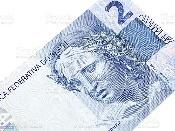
\includegraphics[width=0.79592in,height=0.59694in]{media/image47.jpg} &
TARTARUGA MARINHA & AZUL & dois REAIS\tabularnewline
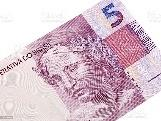
\includegraphics[width=0.73274in,height=0.54956in]{media/image48.jpg} &
GARÇA & ROSA & cinco REAIS\tabularnewline
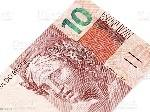
\includegraphics[width=0.68163in,height=0.51122in]{media/image49.jpg} &
ARARA VERMELHA & VERMELHA & dez REAIS\tabularnewline
\includegraphics[width=0.63139in,height=0.41990in]{media/image50.jpg} &
MICO LEÃO DOURADO & AMARELA & vinte REAIS\tabularnewline
\includegraphics[width=0.63326in,height=0.42114in]{media/image51.jpg} &
ONÇA PINTADA & LARANJA & cinquenta REAIS\tabularnewline
\includegraphics[width=0.62794in,height=0.47095in]{media/image52.jpg} &
GAROUPA & AZUL & cem REAIS\tabularnewline
\includegraphics[width=0.63126in,height=0.42104in]{media/image53.jpg} &
LOBO GUARÁ & BRANCA & duzentos REAIS\tabularnewline
\bottomrule
\end{longtable}

Professor(a), é importante que as crianças usem as peculiaridades de
cada cédula, como a cor predominante e o animal contido nela, para
identificar os eu valor. Se possível, mostre aos alunos cédulas
verdadeiras, com o intuito de lhes mostrar a marca d'agua e outras
características que apontem para sua autenticidade.

agora observe as moedas e perceba suas diferenças. se dividirmos um real
em cem partes encontramos 1 centavo. as moedas servem para comprarmos
coisas que custam menos de 1 real. a maior moeda vale exatamente 1 real.

\textless{}https://br.freepik.com/fotos-gratis/dinheiro-moedas-brasileiras-escada\_23076933.htm\#page=9\&query=REAIS\%20moedas\&position=39\&from\_view=search\&track=ais\textgreater{}

\includegraphics[width=5.90556in,height=1.41667in]{media/image54.jpg}\protect\hypertarget{_heading=h.eii4svey01jf}{}{}

\subsection{ATIVIDADES}\label{atividades-4}

\subsubsection{01}\label{section-54}

marque o valor dos produtos nas etiquetas:

\textless{}https://br.freepik.com/vetores-gratis/colecao-de-brinquedos-de-natal-desenhada-a-mao\_11105919.htm\#query=brinquedos\%20com\%20etiquetas\&position=14\&from\_view=search\&track=ais.
Inserir na coluna da direita uma figura de etiqueta para o aluno
preencher o valor da mercadoria.\textgreater{}

\begin{longtable}[]{@{}lll@{}}
\toprule
\includegraphics[width=1.70857in,height=2.10446in]{media/image55.png} &
Cento e trinta e cinco reais e vinte centavos. &
\includegraphics[width=2.19822in,height=2.44826in]{media/image56.png}\tabularnewline
\bottomrule
\end{longtable}

135,20

\begin{longtable}[]{@{}lll@{}}
\toprule
\includegraphics[width=1.16683in,height=1.08348in]{media/image57.png} &
cinquenta e cinco reais e vinte e cinco centavos. &
\includegraphics[width=2.19822in,height=2.44826in]{media/image56.png}\tabularnewline
\bottomrule
\end{longtable}

55,25

\begin{longtable}[]{@{}lll@{}}
\toprule
\includegraphics[width=1.96902in,height=1.29185in]{media/image58.png} &
noventa e oito reais. &
\includegraphics[width=2.19822in,height=2.44826in]{media/image56.png}\tabularnewline
\bottomrule
\end{longtable}

98,00

\begin{longtable}[]{@{}lll@{}}
\toprule
\includegraphics[width=1.60439in,height=1.38561in]{media/image59.png} &
quarenta e dois reais e noventa e nove centavos. &
\includegraphics[width=2.19822in,height=2.44826in]{media/image56.png}\tabularnewline
\bottomrule
\end{longtable}

42,99

\subsubsection{02}\label{section-55}

escreva os valores em reais por extenso.

\textless{}Inserir a tabela conforme o modelo abaixo\textgreater{}

\begin{longtable}[]{@{}ll@{}}
\toprule
R\$ 135,60 & Cento e trinta e cinco reais e sessenta
centavos.\tabularnewline
R\$ 465,00 & Quatrocentos e sessenta e cinco reais.\tabularnewline
R\$ 59,30 & Cinquenta e nove reais e trinta centavos.\tabularnewline
R\$ 74,15 & Setenta e quatro reais e quinze centavos.\tabularnewline
R\$ 63,20 & Sessenta e três reais e vinte centavos.\tabularnewline
R\$ 15,15 & Quinze reais e quinze centavos.\tabularnewline
\bottomrule
\end{longtable}

Professor(a), nas duas atividades anteriores é importante que o aluno se
acostume com as nomenclaturas do dinheiro, a simbologia e etc. Pode
auxiliar no processo de alfabetização e nas habilidades de leitura e
escrita.

\subsubsection{03}\label{section-56}

ligue corretamente os valores às imagens.

\textless{}https://br.freepik.com/fotos-gratis/dinheiro-moedas-brasileiras-1-real\_22809605.htm\#query=moeda\%20de\%201\%20real\%20dineiro\%20barssileiro\&position=1\&from\_view=search\&track=ais;
https://br.freepik.com/fotos-gratis/dinheiro-moedas-brasileiras-5-centavos\_22781620.htm\#query=moeda\%20de\%205\%20centavos\%20dineiro\%20barssileiro\&position=2\&from\_view=search\&track=ais;
https://br.freepik.com/fotos-gratis/dinheiro-moedas-brasileiras-10-centavos\_22781622.htm\#query=moeda\%20de\%2010\%20centavos\%20dineiro\%20barssileiro\&position=6\&from\_view=search\&track=ais;

\begin{longtable}[]{@{}ll@{}}
\toprule
R\$ 0,05 &
\includegraphics[width=0.80577in,height=0.79447in]{media/image60.jpg}\tabularnewline
R\$ 0,50 &
\includegraphics[width=0.69145in,height=0.53632in]{media/image61.jpg}\tabularnewline
R\$ 0,25 &
\includegraphics[width=0.75523in,height=0.67928in]{media/image62.jpg}\tabularnewline
R\$ 0,10 &
\includegraphics[width=0.67617in,height=0.63139in]{media/image63.jpg}\tabularnewline
R\$ 1,00 &
\includegraphics[width=0.69044in,height=0.66964in]{media/image64.jpg}\tabularnewline
\bottomrule
\end{longtable}

Professor(a), os alunos podem ter alguma dificuldade com essa atividade,
uma vez, que ainda não tiveram contato com números fracionários. Aqui o
mais importante é associarem os valores às imagens das moedas.

\subsubsection{04}\label{section-57}

preencha os quadrados com a quantidade de cédulas que precisamos usar
para comprar os seguintes itens:

\textless{}https://www.istockphoto.com/br/foto/notas-de-dinheiro-do-brasil-em-composto-detalhes-de-notas-de-200-50-10-5-e-2-reais-gm1280319451-378658163?phrase=200\%20REAIS.
Inserir quadros para que os alunos consigam colocar a quantidade de
notas necessárias.\textgreater{}

\begin{enumerate}
\def\labelenumi{\Alph{enumi})}
\item
  um carrinho de r\$ 100,00.
\end{enumerate}

\includegraphics[width=5.90556in,height=2.19028in]{media/image65.png}

\begin{enumerate}
\def\labelenumi{\Alph{enumi})}
\item
  uma boneca de R\$ 70,00.
\end{enumerate}

\includegraphics[width=5.90556in,height=2.18611in]{media/image66.png}

\begin{enumerate}
\def\labelenumi{\Alph{enumi})}
\item
  uma calça de R\$ 137,00.
\end{enumerate}

\includegraphics[width=5.90556in,height=2.12778in]{media/image67.png}

\begin{enumerate}
\def\labelenumi{\Alph{enumi})}
\item
  uma saia de R\$ 85,00.
\end{enumerate}

\includegraphics[width=5.90556in,height=2.18056in]{media/image68.png}

\begin{enumerate}
\def\labelenumi{\Alph{enumi})}
\item
  um chocolate de R\$ 6,00.
\end{enumerate}

\includegraphics[width=5.90556in,height=2.14583in]{media/image69.png}

\begin{enumerate}
\def\labelenumi{\Alph{enumi})}
\item
  Um óculos escuro de R\$ 450,00.
\end{enumerate}

\includegraphics[width=5.90556in,height=2.19931in]{media/image70.png}

Professor(a), nessa atividade podemos ter várias configurações
diferentes, exceto no chocolate de R\$ 6,00. É de suma importância
trabalhar com os alunos as respostas diferentes que eles não deram.

\subsubsection{05}\label{section-58}

preencha os círculos com a quantidade de moedas que precisamos usar para
comprar os seguintes itens:

\begin{quote}
\textless{}https://br.freepik.com/fotos-gratis/dinheiro-moedas-brasileiras-escada\_23076933.htm\#page=9\&query=REAIS\%20moedas\&position=39\&from\_view=search\&track=ais.
Inserir os círculos abaixo de cada moeda para o aluno preencher a
quantidade necessária.\textgreater{}
\end{quote}

\begin{enumerate}
\def\labelenumi{\Alph{enumi})}
\item
  um pirulito de R\$ 0,35 (trinta e cinco centavos).
\end{enumerate}

\includegraphics[width=4.34436in,height=1.66690in]{media/image71.png}

\begin{enumerate}
\def\labelenumi{\Alph{enumi})}
\item
  uma bala de R\$ 0,15 (quinze centavos).
\end{enumerate}

\includegraphics[width=4.41728in,height=1.68774in]{media/image72.png}

\begin{enumerate}
\def\labelenumi{\Alph{enumi})}
\item
  Um apito de R\$ 0,30 (trinta centavos).
\end{enumerate}

\includegraphics[width=4.35477in,height=1.63565in]{media/image73.png}

\begin{enumerate}
\def\labelenumi{\Alph{enumi})}
\item
  um chaveiro de super herói de r\$ 3,75 (três reais e setenta e cinco
  centavos).
\end{enumerate}

\includegraphics[width=4.39645in,height=1.81275in]{media/image74.png}

Professor(a), siga as mesmas orientações da atividade anterior.
Lembre-se que nessa atividade os alunos precisarão mais de sua ajuda,
uma vez que ainda não conhecem números fracionários.

\subsubsection{06}\label{section-59}

João e bianca ganahram 10 reais cada um. joão comprou um doce de 6 reais
e bianca um doce de 5 reais. responda com números e escrito por extenso:

\begin{enumerate}
\def\labelenumi{\Alph{enumi})}
\item
  quanto joão e bianca ganharam juntos?
\end{enumerate}

\textless{}2 linhas\textgreater{}

10 + 10 = R\$ 20,00 -- Vinte reais.

\begin{enumerate}
\def\labelenumi{\Alph{enumi})}
\item
  Quanto joão e bianca gastaram juntos?
\end{enumerate}

\textless{}2 linhas\textgreater{}

6 + 5 = R\$ 11,00 - Onze reais.

\begin{enumerate}
\def\labelenumi{\Alph{enumi})}
\item
  com quanto dinheiro ficaram joão e bianca juntos?
\end{enumerate}

\textless{}2 linhas\textgreater{}

(10-6) + (10-5) = 4+5 = R\$ 9,00 - Nove reais.

\begin{enumerate}
\def\labelenumi{\arabic{enumi}.}
\item
  desenhe e pinte as cédulas e moedas do real. não esqueça de nenhum
  detalhe.
\end{enumerate}

\textless{} Inserir um quadro que tome toda uma página, para que os
alunos desenhem as cédulas e moedas.\textgreater{}

Professor(a). permita que os alunos expressem o que aprenderam de forma
lúdica. É importante perceber se conseguem identificar o valor das
moedas pelas cores que vão escolher e pelos animais que vão desenhar.
Lembre-se que nossas habilidades trabalhadas para esse módulo tem uma
grande importância vsual.

\subsection{TREINO}\label{treino-4}

\subsubsection{01}\label{section-60}

Indique o valor da cédula de dinheiro da figura.

\textless{}https://www.istockphoto.com/br/foto/brasileiro-dinheiro-novo-gm492494099-40521892?phrase=10\%20REAIS\textgreater{}

\includegraphics[width=1.92157in,height=1.43284in]{media/image75.png}

A) R\$ 0,10

B) R\$ 1,00

C) R\$ 10,00

D) R\$ 100,00

SAEB: 2M1.7 - Relacionar valores de moedas e/ou cédulas do sistema
monetário brasileiro, com base nas imagens desses objetos.

BNCC: (EF01MA19) Reconhecer e relacionar valores de moedas e cédulas do
sistema monetário brasileiro para resolver situações simples do
cotidiano do estudante.

a) Incorreta. O aluno confundiu a cédula com uma moeda de 10 centavos.

b) Incorreta. O aluno confundiu a cédula com uma moeda de 1 real.

c) Correta. A cédula é de 10 reais.

d) Incorreta. O aluno confundiu a cédula com outra cédula de 100 reais.

\subsubsection{02}\label{section-61}

Cristiano comprou um chapéu de R\$ 75,00. indique como ele pagou.

A) com três cédulas de R\$ 50,00

B) com três cédulas de R\$ 25,00

C) com três cédulas de r\$ 10,00

D) comtrês cédulas de R\$ 5,00

SAEB: 2M2.3 - Resolver problemas que envolvam moedas e/ou cédulas do
sistema monetário brasileiro.

BNCC: (EF01MA19) Reconhecer e relacionar valores de moedas e cédulas do
sistema monetário brasileiro para resolver situações simples do
cotidiano do estudante.

a) Incorreta. Essa composição resulta em R\$ 150,00.

b) Correta. Essa composição resulta corretamente em R\$ 75,00.

c) Incorreta. Essa composição resulta em R\$ 30,00.

d) Incorreta. Essa composição resulta em R\$ 15,00.

\subsubsection{03}\label{section-62}

indique qual composição \textbf{não} forma R\$ 30,00.

A) 30 moedas de 1 real.

B) 3 cédulas de 10 reais.

C) 1 cédula de 25 reais mais uma de 5 reais.

D) 1 cédula de 10 reais mais uma de 5 reais.

SAEB: 2M2.3 - Resolver problemas que envolvam moedas e/ou cédulas do
sistema monetário brasileiro.

BNCC: (EF01MA19) Reconhecer e relacionar valores de moedas e cédulas do
sistema monetário brasileiro para resolver situações simples do
cotidiano do estudante.

a) Incorreta. Pois a composição de 30 moedas de 1 real resulta em 30
reais.

b) Incorreta. Pois a composição de 3 cédulas de 10 reais resulta em 30
reais.

c) Incorreta. Pois a composição de 1 cédula de 25 mais 5 resulta em 30
reais.

d) Correta. Pois a composição de 1 cédula de 10 reais mais 5 resulta em
15 reais, diferente de 30 reais.

\section{MÓDULO 6: SERÁ QUE VAI
CHOVER?}\label{muxf3dulo-6-seruxe1-que-vai-chover}

Neste módulo vamos trabalhar a habilidade que desenvolve nos alunos a
percepção de que alguns fatos podem ser previsíveis e outros não. A
noção de probabilidade matemática pode ser um pouco complexa para
crianças dessa idade, porém, utilizando situações do cotidiano dessa
criança podemos faze-la perceber que é mais provável que algumas coisas
aconteçam em detrimento a outras coisas. Habilidade da BNCC: EF01MA20

Habilidade do SAEB:

- Classificar resultados de eventos cotidianos aleatórios como ``pouco
prováveis'', ``muito prováveis'', ``certos'' ou ``impossíveis''.

\subsection{CONTEÚDO}\label{conteuxfado-5}

você já se perguntou sobre como é possivel saber se vai ou não chover?
se olharmos para o céu e vê-lo escuro sabemos que vai chover. mas, como
eles conseguem prever isso uma semana antes? uma série de acontecimentos
permitem aos técnicos fazer uma previsão. nós também podemos prever
algumas coisas no nosso dia a dia. para isso, precisamos pensar em
quatro possibilidades. observe o quadro:

\textless{}Inserir um quadro conforme o modelo a seguir, utilizando as
referências:
https://br.freepik.com/vetores-premium/pequeno-elefante-voar-para-o-ceu\_6579577.htm\#query=elefante\%20voando\&position=9\&from\_view=search\&track=ais;
https://br.freepik.com/vetores-gratis/fundo-plano-do-polo-norte-da-temporada-de-inverno\_33138109.htm\#query=neve\&position=11\&from\_view=search\&track=sph
(alterar a placa colocando nela Brasil no lugar de polo norte.;
https://br.freepik.com/vetores-gratis/ilustracao-de-calor-de-verao-plana-com-homem-na-cadeira\_27995494.htm\#query=ver\%C3\%A3o\%20calor\&position=0\&from\_view=search\&track=ais;
https://br.freepik.com/vetores-premium/jogador-de-futebol-jogando-futebol-em-pe\_33803714.htm\#query=bola\%20jogada\%20pra\%20cima\&position=7\&from\_view=search\&track=ais.\textgreater{}

\begin{longtable}[]{@{}llll@{}}
\toprule
impossível & quando não existe a menor chancer de algo acontecer. & um
elefante sair voando por conta própria. &
\includegraphics[width=1.42708in,height=1.42708in]{media/image76.jpg}\tabularnewline
pouco provável & quando existe uma pequena chance de algo acontecer. &
nevar no brasil. &
\includegraphics[width=1.52602in,height=1.01167in]{media/image77.png}\tabularnewline
muito provável & quando existe uma grande chance de algo acontecer. &
fazer calor no verão. &
\includegraphics[width=1.30208in,height=1.30208in]{media/image78.jpg}\tabularnewline
certeza & quando é certo que algo vai acontecer. & uma bola cair quando
for jogada pra cima. &
\includegraphics[width=1.04437in,height=1.39696in]{media/image79.jpg}\tabularnewline
\bottomrule
\end{longtable}

Professor(a), é importante ressaltar com os alunos que no Brasil é raro
nevar, mas que pode acontecer, principalmente na região sul. Vale
ressaltar também que nem todos os dias do verão são quentes, ou seja, a
temperatura pode cair em alguns dias.

\subsection{ATIVIDADES}\label{atividades-5}

\subsubsection{01}\label{section-63}

pinte os círculos com as situações impossíveis no quadro abaixo. pinte
da cor que você quiser.

\textless{}criar um quadro com as situações descritas conforme o modelo
a seguir.\textgreater{}

\includegraphics[width=5.16074in,height=7.09420in]{media/image80.png}

Professor(a), essa atividade pode ser importante para trabalhar a
habilidade de leitura dos alunos. As situações impossíveis são: céu
ficando verde, tesoura falando, jacaré voando, leão miando, unicórnios,
chuva caindo pra cima e árvore andando.

\subsubsection{02}\label{section-64}

desenhe nos quadros abaixo duas situações que você considere
impossíveis. não vale repetir as situações da atividade anterior.

\textless{}Inserir dois quadros para os alunos desenharem, tomando toda
a página\textgreater{}

\includegraphics[width=4.38938in,height=7.65199in]{media/image81.png}

Professor(a), nessa atividade você deve permitir que o aluno utilize sua
imaginação infantil sem moderação. Começar com os acontecimentos
impossíveis é importante, pois permite que o aluno utilize sua
imaginação infantil, provocando engajamento e envolvimento na criança.

\subsubsection{03}\label{section-65}

ligue as situações com as imagens corretamente.

\textless{}https://br.freepik.com/vetores-gratis/chovendo-na-natureza-paisagem\_5769787.htm\#query=rel\%C3\%A3mpago\%20na\%20chuva\&position=6\&from\_view=search\&track=ais;
https://br.freepik.com/vetores-gratis/tartaruga-jogando-skate-no-parque\_4119896.htm\#query=sapo\%20jogando\%20volei\&position=0\&from\_view=search\&track=ais;

\begin{longtable}[]{@{}ll@{}}
\toprule
\begin{minipage}[t]{0.48\columnwidth}\raggedright\strut
\includegraphics[width=2.03487in,height=1.82023in]{media/image82.jpg}

relampiar na chuva\strut
\end{minipage} & \begin{minipage}[t]{0.48\columnwidth}\raggedright\strut
impossível\strut
\end{minipage}\tabularnewline
\begin{minipage}[t]{0.48\columnwidth}\raggedright\strut
\includegraphics[width=2.11035in,height=1.45968in]{media/image83.jpg}

tartaruga \emph{skatista.}\strut
\end{minipage} & \begin{minipage}[t]{0.48\columnwidth}\raggedright\strut
pouco provável\strut
\end{minipage}\tabularnewline
\begin{minipage}[t]{0.48\columnwidth}\raggedright\strut
\includegraphics[width=2.11129in,height=1.37616in]{media/image84.jpg}

acidente aéreo.\strut
\end{minipage} & \begin{minipage}[t]{0.48\columnwidth}\raggedright\strut
muito provável\strut
\end{minipage}\tabularnewline
\begin{minipage}[t]{0.48\columnwidth}\raggedright\strut
\includegraphics[width=1.86458in,height=1.86458in]{media/image85.jpg}

você sentir fome\strut
\end{minipage} & \begin{minipage}[t]{0.48\columnwidth}\raggedright\strut
certeza\strut
\end{minipage}\tabularnewline
\bottomrule
\end{longtable}

\subsubsection{04}\label{section-66}

preencha com um x as possibilidades do quadro abaixo.

\begin{longtable}[]{@{}lllll@{}}
\toprule
situação & impossível & pouco provável & muito provável &
certeza\tabularnewline
esquecer de escovar os dentes. & & & &\tabularnewline
esquecer de fazer a lição. & & & &\tabularnewline
jogar \emph{video game} todo o dia. & & & &\tabularnewline
sentir vontade de ir ao banheiro. & & & &\tabularnewline
brincar com o papai. & & & &\tabularnewline
brincar com a mamãe. & & & &\tabularnewline
brincar com os amiguinhos. & & & &\tabularnewline
esquecer a luz acesa. & & & &\tabularnewline
esquecer de dar a descarga depois de usar o banheiro. & & &
&\tabularnewline
comer doces fora de hora. & & & &\tabularnewline
assitir tv ou ficar na internet na hora de comer. & & & &\tabularnewline
\bottomrule
\end{longtable}

Professor(a), nessa atividade podemos auxiliar o aluno a fazer uma auto
avaliação de como ele administra seu tempo diariamente, além de ajuda-lo
a criar suas prioridades. Essa atividade favorece o trabalho com as TCTs
Sáude e Vida familiar e social.

\subsubsection{05}\label{section-67}

zélia estava brincando de jogar o seu dado. pinte no quadro abaixo quais
os resultados prováveis de sairem quando zélia jogar uma vez.

\begin{longtable}[]{@{}llll@{}}
\toprule
\includegraphics[width=1.55208in,height=1.55208in]{media/image86.jpg} &
1 & 15 & 6\tabularnewline
& 20 & 3 & 8\tabularnewline
& 5 & 10 & 9\tabularnewline
& 11 & 4 & 12\tabularnewline
& 13 & 14 & 2\tabularnewline
\bottomrule
\end{longtable}

Professor(a), é importante que o aluno perceba que só podem sair os
resultados de 1 a 6. Visto que são os únicos números que temos em um
dado. Se possível, distribua ou mostre um dado para os alunos durante a
atividade.

\subsubsection{06}\label{section-68}

DESCUBRA QUAL DOS JOGADORES ABAIXO TEM A MAIOR CHANCE DE GANHAR O JOGO
DE DOMINÓS. CIRCULE O NOME DESSE JOGADOR.

\textless{}https://br.freepik.com/vetores-gratis/ilustracao-realista-de-jogo-de-domino\_22656073.htm\#query=domin\%C3\%B3\%20jogada\&position=29\&from\_view=search\&track=ais;
https://br.freepik.com/vetores-premium/stock-vector-domino-conjunto-completo-ilustracao-realista-colecao-de-cartoes-de-domino-de-cor-preto-e-branco\_22221437.htm\#query=domin\%C3\%B3\%20jogada\&position=35\&from\_view=search\&track=ais\textgreater{}

\includegraphics[width=4.84499in,height=2.71476in]{media/image87.png}

Professor(a), é importante que o aluno perceba que Solange é a única
jogadora que possui uma pedra com o número 5. Nenhum outro jogador
possui uma pedra assim ,logo, a chance de vitória de Solange é maior.

\subsubsection{07}\label{section-69}

bernardo está brincnando de colocar diferentes tipos de bola na água
para ver se flutua. você consegue prever qual será o resultado? assinale
com x nas caixinhas.

\textless{}Inserir quadro conforme o modelo a seguir, utilizando as
referências:
https://br.freepik.com/fotos-premium/bola-de-papel-amassado\_25578632.htm?query=bola\%20de\%20papel\#from\_view=detail\_alsolike
https://br.freepik.com/vetores-premium/bola-de-cromo-3d-realista-isolada-no-fundo-branco\_34098681.htm\#query=bola\%20de\%20metal\&position=24\&from\_view=search\&track=ais;
https://br.freepik.com/vetores-premium/esfera-branca-bola-ilustracao\_9402860.htm\#query=bola\%20de\%20isopor\&position=13\&from\_view=search\&track=ais;
https://br.freepik.com/vetores-premium/bola-de-bilhar\_26468289.htm\#query=bola\%20de\%20bilhar\&position=46\&from\_view=search\&track=ais
\textgreater{}

\begin{longtable}[]{@{}llll@{}}
\toprule
\begin{minipage}[t]{0.24\columnwidth}\raggedright\strut
\includegraphics[width=1.06165in,height=0.99037in]{media/image88.jpg}

Bola de papel flutua?\strut
\end{minipage} & \begin{minipage}[t]{0.24\columnwidth}\raggedright\strut
\includegraphics[width=0.98125in,height=0.98125in]{media/image89.jpg}

Bola de metal flutua?\strut
\end{minipage} & \begin{minipage}[t]{0.24\columnwidth}\raggedright\strut
\includegraphics[width=0.83333in,height=0.83333in]{media/image90.jpg}

Bola de isopor flutua?\strut
\end{minipage} & \begin{minipage}[t]{0.24\columnwidth}\raggedright\strut
\includegraphics[width=0.83333in,height=0.83333in]{media/image91.jpg}

Bola de bilhar flutua?\strut
\end{minipage}\tabularnewline
sim & & sim &\tabularnewline
não & & não &\tabularnewline
talvez & & talvez &\tabularnewline
\bottomrule
\end{longtable}

Professor(a), nessa atividade, ainda que os alunos não conheçam o
conceito de flutuabilidade ou princípio de Arquimedes, é importante
desenvolver suas habilidades de prever um acontecimento, baseados no
senso comum, ou até em experiências pessoais. Alguns alunos podem ter
manipulado algumas dessas bolas, ou até mesmo feito alguma experiência
desse tipo. Se julgar necessário, e for possível, faça a experiência em
sala de aula. Você pode promover um game de adivinhação, promovendo
maior engajamento dos alunos. Aqui não é viável entrar no conceito de
densidade por ser um assunto muito complexo para a idade, porém, deve-se
tomar cuidado para não criar um subsunçor na estrutura cognitiva do
aluno acerca da massa das bolas, sendo o fator determinante para a
flutuação. Cuidado!

\subsubsection{08}\label{section-70}

discuta uma situação com os colegas que seja muito provável e desenhe
essa situação no quadro abaixo. descreva que situação é essa.

\textless{}Inserir um quadro para o aluno desenhar além de duas linhas
para o aluno descrever a situação. Essa atividade deve preencher uma
página\textgreater{}

\includegraphics[width=3.24914in,height=2.92171in]{media/image92.png}

Professor(a), aproveite essa atividade para desenvolver a habilidade de
escrita. Oriente os alunos quanto a escolha da situação.

\subsubsection{09}\label{section-71}

discuta uma situação com os colegas que seja pouco provável e desenhe
essa situação no quadro abaixo. descreva que situação é essa.

\textless{}Inserir um quadro para o aluno desenhar além de duas linhas
para o aluno descrever a situação. Essa atividade deve preencher uma
página\textgreater{}

\includegraphics[width=2.86272in,height=2.57423in]{media/image92.png}

Professor(a), siga as orientações da atividade anterior.

\subsubsection{10}\label{section-72}

discuta uma situação com os colegas que seja uma certeza e desenhe essa
situação no quadro abaixo. descreva que situação é essa.

\textless{}Inserir um quadro para o aluno desenhar além de duas linhas
para o aluno descrever a situação. Essa atividade deve preencher uma
página\textgreater{}

\includegraphics[width=2.86272in,height=2.57423in]{media/image92.png}

Professor(a), siga as orientações da atividade anterior.

\subsection{TREINO}\label{treino-5}

\subsubsection{01}\label{section-73}

indique qual dessas situações é impossível de acontecer.

A) uma caneta escrevendo.

B) um gato dormindo.

C) um navio flutuando

D) um peixe escalando uma montanha

SAEB: - Classificar resultados de eventos cotidianos aleatórios como
``pouco prováveis'', ``muito prováveis'', ``certos'' ou ``impossíveis''.

BNCC: (EF01MA20) Classificar eventos envolvendo o acaso, tais como
``acontecerá com certeza'', ``talvez aconteça'' e ``é impossível
acontecer'', em situações do cotidiano.

a) Incorreta. Uma caneta é feita para escrever.

b) Incorreta. Gatos também dormem.

c) Incorreta. Todo navio foi feito para flutuar

d) Correta. Peixes não vivem fora da água.

\subsubsection{02}\label{section-74}

Indique qual dessas situações é pouco provável de acontecer.

A) fazer calor no verão

B) fazer frio no verão.

C) nevar no inverno.

D) surgirem flores nas árvores na primavera.

SAEB: - Classificar resultados de eventos cotidianos aleatórios como
``pouco prováveis'', ``muito prováveis'', ``certos'' ou ``impossíveis''.

BNCC: (EF01MA20) Classificar eventos envolvendo o acaso, tais como
``acontecerá com certeza'', ``talvez aconteça'' e ``é impossível
acontecer'', em situações do cotidiano.

a) Incorreta. É muito provável que faça calor no verão.

b) Correta. É pouco provável que faça frio no verão, ainda que seja
possível.

c) Incorreta. É muito provável que neve caia no inverno, principalmente
no hemisfério norte do planeta.

d) Incorreta. É certeza que as árvores floresçam na primavera.

\subsubsection{03}\label{section-75}

Indique qual dos números a seguir \textbf{não} poderá ser sorteado em
uma jogada de dados

A) 3

B) 5

C) 6

D) 7

\protect\hypertarget{_heading=h.30j0zll}{}{}SAEB: - Classificar
resultados de eventos cotidianos aleatórios como ``pouco prováveis'',
``muito prováveis'', ``certos'' ou ``impossíveis''.

BNCC: (EF01MA20) Classificar eventos envolvendo o acaso, tais como
``acontecerá com certeza'', ``talvez aconteça'' e ``é impossível
acontecer'', em situações do cotidiano.

a) Incorreta. Em um dado de 1 a 6, o número 3 é uma possibilidade.

b) Incorreta. Em um dado de 1 a 6, o número 5 é uma possibilidade.

c) Incorreta. Em um dado de 1 a 6, o número 6 é uma possibilidade.

d) Correta. Em um dado de 1 a 6, o número 7 não é uma possibilidade.

\section{MÓDULO 7: TUDO
ORGANIZADINHO!}\label{muxf3dulo-7-tudo-organizadinho}

Neste módulo vamos desenvolver nos alunos a habilidade de identificar e
colocar informações em gráficos e tabelas.

Habilidades da BNCC: EF01MA21 e EF01MA22.

Habilidades da SAEB:

- Ler/identificar ou comparar dados estatísticos ou informações,
expressos em tabelas (simples ou de dupla entrada).

- Ler/identificar ou comparar dados estatísticos expressos em gráficos
(barras simples, colunas simples ou pictóricos).

- Representar os dados de uma pesquisa estatística ou de um levantamento
em listas, tabelas (simples ou de dupla entrada) ou gráficos (barras
simples, colunas simples ou pictóricos).

\subsection{CONTEÚDO}\label{conteuxfado-6}

você já percebeu como algumas informações ficam organizadas? como listas
de compras da mamãe, como a lsita de materiais da escola, ou então o
\emph{ranking} daquele seu \emph{game} favorito? pois é! essas são as
tabelas e gráficos. observe a imagem abaixo:

\textless{}Inserir a referência:
https://br.freepik.com/vetores-gratis/tabela-de-classificacao-com-fundo-abstrato\_11187227.htm\#query=score\%20game\&position=0\&from\_view=search\&track=ais.
Não é necessário traduzir. Os alunos estão habituados a \emph{games} e
suas terminologias nessa idade.\textgreater{}

\includegraphics[width=1.77083in,height=1.77083in]{media/image93.jpg}

a classificação e os pontos dos jogadores desse jogo são apresentados em
uma tabela. como temos duas informações, ou seja, a classificação e a
potuação, dizemos que é uma tabela de dupla entrada.

temos também os gráficos de barras e de figuras. observe.

\textless{}Criar gráficos conforme o modelo a seguir.\textgreater{}

{{[}CHART{]}}\includegraphics[width=3.13415in,height=1.79094in]{media/image94.png}

Em uma turma de 1° ano perguntaram para que time as crianças torciam. o
resultado está nesses gráficos. perceba que a maioria das crianças
torciam para o corinthians. os gráficos nos ajudam a perceber essas
coisas mais facilmente. Você saberia me dizer, só olhando para eles,
qual time foi o menos escolhido?

\subsection{ATIVIDADES}\label{atividades-6}

\subsubsection{01}\label{section-76}

analise a tabela, que mostra pontuação de jogadores de uma partida de
boliche, e responda:

\textless{}Inserir tabela conforme o modelo a seguir. Inserir a
referência:
https://br.freepik.com/vetores-premium/jogador-de-boliche\_2938032.htm\#query=boliche\%20crian\%C3\%A7as\&position=5\&from\_view=search\&track=ais.\textgreater{}

\includegraphics[width=1.88542in,height=1.88542in]{media/image95.jpg}

\begin{longtable}[]{@{}ll@{}}
\toprule
jogador & pontuação\tabularnewline
\midrule
\endhead
marcos & 46\tabularnewline
ricardo & 56\tabularnewline
suzana & 32\tabularnewline
hévilin & 31\tabularnewline
débora & 47\tabularnewline
lucas & 35\tabularnewline
marcelo & 35\tabularnewline
\bottomrule
\end{longtable}

\begin{enumerate}
\def\labelenumi{\Alph{enumi})}
\item
  quem fez mais pontos?
\end{enumerate}

\textless{}1 linha\textgreater{}

Ricardo tem a maior pontuação.

\begin{enumerate}
\def\labelenumi{\Alph{enumi})}
\item
  quem fez menos pontos?
\end{enumerate}

\textless{}1 linha\textgreater{}

Hévilin tem a menor pontuação.

\begin{enumerate}
\def\labelenumi{\Alph{enumi})}
\item
  houve algum empate?
\end{enumerate}

\textless{}1 Linha\textgreater{}

Lucas e Marcelo empataram fazendo ambos 35 pontos.

\begin{enumerate}
\def\labelenumi{\Alph{enumi})}
\item
  preencha o podium com os nomes do 1°, 2° e 3° colocados.
\end{enumerate}

\textless{}Inserir referência acrescentando os quadros para o aluno
preencher o nome.\textgreater{}

\includegraphics[width=5.90556in,height=3.03472in]{media/image96.png}

Professor(a), oriente os alunos a buscarem as informações pedidas na
tabela.

\subsubsection{02}\label{section-77}

no 1° ano foi feita uma pesquisa para saber que tipo de alimentos as
crianças mais comiam. o resultado está no grÁfico a seguir. OBSERVE E
RESPONDA.

\textless{}Inserir gráfico conforme o modelo a seguir.\textgreater{}

{{[}CHART{]}}

\begin{enumerate}
\def\labelenumi{\Alph{enumi})}
\item
  qual a comida preferida do 1° ano?
\end{enumerate}

\textless{}1 linha\textgreater{}

A maioria dos alunos preferem massas.

\begin{enumerate}
\def\labelenumi{\Alph{enumi})}
\item
  qual a comida menos querida do 1° ano?
\end{enumerate}

\textless{}1 linha\textgreater{}

A minoria dos alunos costuma comer verduras.

\begin{enumerate}
\def\labelenumi{\Alph{enumi})}
\item
  qual a segunda comida preferida dos alunos do 1° Ano?
\end{enumerate}

\textless{}1 Linha\textgreater{}

Os doces são a segunda comida preferida dos alunos.

\begin{enumerate}
\def\labelenumi{\Alph{enumi})}
\item
  é mais provável que os alunos do 1° ano sejam gordinhos ou magrinhos?
  explique sua resposta.
\end{enumerate}

\textless{}3 linhas\textgreater{}

Professor(a), é importante que os alunos percebam que o fato de os
alunos comerem mais massas e doces faça com que seja mais provável
encontrarmos alunos mais gordinhos. Essa atividade favorece uma
discussão acerca da obesidade infantil, assim como o trabalho com a
TCT-Educação alimentar e nutricional.

\subsubsection{03}\label{section-78}

a tabela mostra a lista dos jogos mais jogados e mais curtidos pelos
alunos do 1° ano. A tabela também mostra quantos alunos preferem cada
jogo.

\begin{longtable}[]{@{}ll@{}}
\toprule
\emph{minecraft} & 8\tabularnewline
\emph{mario kart 8} & 9\tabularnewline
\emph{animal crossing: new horizons} & 5\tabularnewline
\emph{super mario party} & 3\tabularnewline
\emph{roblox} & 10\tabularnewline
\bottomrule
\end{longtable}

\begin{enumerate}
\def\labelenumi{\Alph{enumi})}
\item
  coloque os jogos em ordem na tabela abaixo. coloque o numero 1 para ao
  mais jogado, número 2 para o segundo mais jogado e assim por diante.
\end{enumerate}

\begin{longtable}[]{@{}ll@{}}
\toprule
\emph{minecraft} & 3\tabularnewline
\emph{mario kart 8} & 2\tabularnewline
\emph{animal crossing: new horizons} & 4\tabularnewline
\emph{super mario party} & 5\tabularnewline
\emph{roblox} & 1\tabularnewline
\bottomrule
\end{longtable}

Professor(a), lembre os alunos sobre a função dos números para ordenar
coisas. Se julgar pertinente, peça para que escrevam primeiro, segundo e
assim por diante, com o fim de trabalhar a habilidade de escrita dos
números ordinais.

\begin{enumerate}
\def\labelenumi{\Alph{enumi})}
\item
  preencha o gráfico abaixo, pintando os quadradinhos, conforme a tabela
  de alunos.
\end{enumerate}

\begin{longtable}[]{@{}llllll@{}}
\toprule
10 & & & & &\tabularnewline
9 & & & & &\tabularnewline
8 & & & & &\tabularnewline
7 & & & & &\tabularnewline
6 & & & & &\tabularnewline
5 & & & & &\tabularnewline
4 & & & & &\tabularnewline
3 & & & & &\tabularnewline
2 & & & & &\tabularnewline
1 & & & & &\tabularnewline
jogos & \emph{minecraft} & \emph{mario kart 8} & \emph{animal crossing:
new horizons} & \emph{super mario party} & \emph{roblox}\tabularnewline
\bottomrule
\end{longtable}

Professor(a), oriente os alunos a transferirem as informações da
primeira tabela para o gráfico de barras. Explique aos alunos que cada
quadradinho é um aluno que escolheu o jogo selecionado. Essa atividade
favorece o trabalho com a TCT -- ciência e tecnologia, assim como a
competência geral 5 da BNCC.

\subsubsection{04}\label{section-79}

vamos brincar de jogar dados? pegue um dado de 6 lados e jogue-o dez
vezes. pinte a quantidade de quadradinhos de cada jogada no gráfico
abaixo.

\textless{}inserir a referência:
https://br.freepik.com/vetores-gratis/ilustracao-de-desenho-de-tatuagem\_33488420.htm\#query=dice\%20kids\&position=4\&from\_view=search\&track=ais.\textgreater{}

\includegraphics[width=1.31250in,height=1.31250in]{media/image97.jpg}

\begin{longtable}[]{@{}lllllllllll@{}}
\toprule
6 \includegraphics[width=0.56258in,height=0.57300in]{media/image98.png}
& & & & & & & & & &\tabularnewline
5 \includegraphics[width=0.53132in,height=0.55216in]{media/image99.png}
& & & & & & & & & &\tabularnewline
4 \includegraphics[width=0.61467in,height=0.53132in]{media/image100.png}
& & & & & & & & & &\tabularnewline
3 \includegraphics[width=0.56258in,height=0.53132in]{media/image101.png}
& & & & & & & & & &\tabularnewline
2 \includegraphics[width=0.57300in,height=0.54174in]{media/image102.png}
& & & & & & & & & &\tabularnewline
1 \includegraphics[width=0.58341in,height=0.55216in]{media/image103.png}
& & & & & & & & & &\tabularnewline
jogadas & 1° & 2° & 3° & 4° & 5° & 6° & 7° & 8° & 9° &
10°\tabularnewline
\bottomrule
\end{longtable}

Professor(a), distribua dados aos alunos, ou então projete um dado
online pelo projetor. Nessa atividade você pode trabalhar questões como
aleatoriedade ou probabilidade, conforme módulo anterior.

\subsubsection{05}\label{section-80}

vamos entender o que é diversidade? vamos fazer uma pesquisa na sala e
depois preencher a tabela abaixo. a pergunta é: qual a sua raça?

\begin{longtable}[]{@{}ll@{}}
\toprule
raça & quantidade de alunos\tabularnewline
\midrule
\endhead
branca &\tabularnewline
preta &\tabularnewline
parda &\tabularnewline
amarela &\tabularnewline
indígena &\tabularnewline
\bottomrule
\end{longtable}

Professor(a), explique aos alunos a diferença da cor de pele de cada
raça, tomando o cuidado para não ser preconceituoso ou jocoso, e
oriente-os a colocarem a quantidade de alunos de cada raça na tabela. É
de suma importância que essa atividade seja utilizada para trabalhar as
TCTs -- Diversidade cultural e Educação para a valorização das
multiculturalidades nas matrizes históricas e culturais brasileiras.

\subsubsection{06}\label{section-81}

Agora vamos desenhar um gráfico de barras com os dados da tabela?

\begin{longtable}[]{@{}llllll@{}}
\toprule
7 & & & & &\tabularnewline
6 & & & & &\tabularnewline
5 & & & & &\tabularnewline
4 & & & & &\tabularnewline
3 & & & & &\tabularnewline
2 & & & & &\tabularnewline
1 & & & & &\tabularnewline
& branca & preta & parda & amarela & indígena\tabularnewline
\bottomrule
\end{longtable}

Professor(a), oriente os alunos a preencherem o gráfico, desenhando
barras que tenham a altura correspondente ao numero de alunos obtidos.
Se a sala tiver mais alunos oriente-os a fazerem a atividade no caderno.

\subsubsection{07}\label{section-82}

a tabela a seguir mostra as temperaturas na cidade de são paulo em cinco
dias quaisquer.

\textless{}Inserir a referência:
https://br.freepik.com/vetores-gratis/contraste-de-inverno-e-verao-clima-frio-e-quente\_18733427.htm\#query=temperatura\&position=26\&from\_view=search\&track=sph.\textgreater{}

\begin{quote}
\includegraphics[width=2.20878in,height=1.47139in]{media/image104.jpg}
\end{quote}

\begin{longtable}[]{@{}lllll@{}}
\toprule
2° feira & 3° feira & 4° feira & 5° feira & 6° feira\tabularnewline
\midrule
\endhead
37° & 35° & 22° & 20° & 19°\tabularnewline
\bottomrule
\end{longtable}

responda:

\begin{enumerate}
\def\labelenumi{\Alph{enumi})}
\item
  qual o dia mais quente dessa semana?
\end{enumerate}

\textless{}1 linha\textgreater{}

2° feira.

\begin{enumerate}
\def\labelenumi{\Alph{enumi})}
\item
  qual o dia mais frio dessa semana?
\end{enumerate}

\textless{}1linha\textgreater{}

6° feira.

\begin{enumerate}
\def\labelenumi{\Alph{enumi})}
\item
  a temperatura está aumentando ou diminuindo?
\end{enumerate}

Professor(a), é importante que o aluno perceba que na segunda feira
temos um número maior representando a temperatura do que o número da
sexta-feira. Nessa atividade podemos trabalhar números ordinais e datas.
Explique aos alunos de forma superficial o que é temperatura.

\begin{enumerate}
\def\labelenumi{\Alph{enumi})}
\item
  desenhe as barras de um gráfico com os dados da tabela.
\end{enumerate}

\begin{longtable}[]{@{}llllll@{}}
\toprule
37 & & & & &\tabularnewline
35 & & & & &\tabularnewline
22 & & & & &\tabularnewline
20 & & & & &\tabularnewline
19 & & & & &\tabularnewline
& 2°feira & 3°feira & 4°feira & 5°feira & 6°feira\tabularnewline
\bottomrule
\end{longtable}

Professor (a) é importante que os alunos percebam que temos barras com
tamanhos decrescentes, em virtude de as temperaturas estarem diminuindo
ao logo da semana.

\subsubsection{08}\label{section-83}

pinte os troféis do gráfico conforme a quantidade de títulos da copa do
mundo da fifa das seleções. confira a tabela.

\begin{longtable}[]{@{}ll@{}}
\toprule
seleção & copas do mundo da fifa\tabularnewline
\midrule
\endhead
brasil & 5\tabularnewline
alemanha & 4\tabularnewline
italia & 4\tabularnewline
argentina & 3\tabularnewline
frança & 2\tabularnewline
uruguai & 2\tabularnewline
espanha & 1\tabularnewline
inglaterra & 1\tabularnewline
\bottomrule
\end{longtable}

\textless{}Inserir um pictograma com as taças da copa para os aluinos
colorir na coluna da direita, conforme o modelo a seguir.\textgreater{}

\begin{longtable}[]{@{}ll@{}}
\toprule
brasil &
\includegraphics[width=3.05575in,height=0.58176in]{media/image105.png}\tabularnewline
alemanha &
\includegraphics[width=3.05575in,height=0.58176in]{media/image105.png}\tabularnewline
italia &
\includegraphics[width=3.05575in,height=0.58176in]{media/image105.png}\tabularnewline
argentina &
\includegraphics[width=3.05575in,height=0.58176in]{media/image105.png}\tabularnewline
frança &
\includegraphics[width=3.05575in,height=0.58176in]{media/image105.png}\tabularnewline
uruguai &
\includegraphics[width=3.05575in,height=0.58176in]{media/image105.png}\tabularnewline
espanha &
\includegraphics[width=3.05575in,height=0.58176in]{media/image105.png}\tabularnewline
inglaterra &
\includegraphics[width=3.05575in,height=0.58176in]{media/image105.png}\tabularnewline
\bottomrule
\end{longtable}

\subsection{TREINO}\label{treino-6}

\subsubsection{01}\label{section-84}

ANALISE O GRÁFICO QUE MOSTRA A PREFERÊNCIA DE FRUTAS DOS ALUNOS DO 1°
ANO E INDIQUE QUAL A FRUTA MAIS ESCOLHIDA.

\begin{quote}
{{[}CHART{]}}
\end{quote}

A) BANANA

B) MAÇA

C) MORANGO

D) PÊRA

SAEB: 2E1.3 - Ler/identificar ou comparar dados estatísticos expressos
em gráficos (barras simples, colunas simples ou pictóricos).

BNCC: (EF01MA21) Ler dados expressos em tabelas e em gráficos de colunas
simples.

a) Incorreta. A banana foi a segunda mais escolhida como a maçã.

b) Incorreta. A maçã foi a segunda mais escolhida como a banana.

c) Correta. O morango foi escolhido 5 vezes, logo foi o mais escolhido.

d) Incorreta. A pêra foi a fruta menos escolhida.

\subsubsection{02}\label{section-85}

Analise a tabela abaixo e indique qual o estilo de música menos ouvido
pelos alunos da escola.

\begin{longtable}[]{@{}ll@{}}
\toprule
ritmo & alunos que ouvem\tabularnewline
\midrule
\endhead
pagode & 2\tabularnewline
rock & 2\tabularnewline
sertanejo & 6\tabularnewline
funk & 2\tabularnewline
clássica & 0\tabularnewline
\bottomrule
\end{longtable}

A) clássica

B) funk

C) rock

D) sertanejo

\protect\hypertarget{_heading=h.1fob9te}{}{}SAEB: 2E1.2 -
Ler/identificar ou comparar dados estatísticos ou informações, expressos
em tabelas (simples ou de dupla entrada).

BNCC: (EF01MA21) Ler dados expressos em tabelas e em gráficos de colunas
simples.

a) Correta. Nenhum aluno da escola ouvia música clássica.

b) Incorreta. O funk é pouco escutado, porém mais do que a música
clássica.

c) Incorreta. O rock é tão ouvido quanto o funk.

d) Incorreta. O sertanejo é o ritmo mais ouvido.

\subsubsection{03}\label{section-86}

INDIQUE QUAL O ESPORTE MENOS ESCOLHIDO PELOS ALUNOS, ANALISANDO O
GRÁFICO ABAIXO.

\begin{quote}
{{[}CHART{]}}
\end{quote}

A) BASQUETE

B) FUTEBOL

C) JUDÔ

D) TÊNIS DE MESA

\protect\hypertarget{_heading=h.3znysh7}{}{}SAEB: 2E1.3 -
Ler/identificar ou comparar dados estatísticos expressos em gráficos
(barras simples, colunas simples ou pictóricos).

BNCC: (EF01MA21) Ler dados expressos em tabelas e em gráficos de colunas
simples.

a) Incorreta. O basquete não foi escolhido.

b) Incorreta. O futebol foi o mais escolhido, com 10 alunos.

c) Incorreta. O judô foi o segundo mais escolhido, com 5 alunos.

d) Incorreta. O tênis de mesa foi o menos escolhido, com 3 alunos.

\section{SIMULADO 1}\label{simulado-1}

\subsubsection{01}\label{section-87}

No pacote de açucar que compramos no supermercado sempre tem um número
1, seguido da unidade kg. o que esse número representa?

A) código de identificação

B) medida

C) quantidade

D) ordem

SAEB: 2N1.1 - Reconhecer o que os números naturais indicam em diferentes
situações: quantidade, ordem, medida ou código de identificação.

BNCC: (EF01MA01) Utilizar números naturais como indicador de quantidade
ou de ordem em diferentes situações cotidianas e reconhecer situações em
que os números não indicam contagem nem ordem, mas sim código de
identificação.

a) Incorreta. Todos os pacotes de açúcar têm esse número, logo, não pode
ser um número de identificação.

b) Correta. O numero um seguido da unidade quilograma indica a medida de
massa do pacote de açúcar.

c) Incorreta. Ainda que esse número indique uma quantidade de açúcar,
essa quantificação traz uma unidade de medida, logo, não é a
quantificação exata de um determinado objeto.

d) Incorreta. Esse número não expressa a posição do pacote em nenhum
lugar.

\subsubsection{02}\label{section-88}

Analise o alfabeto e indique qual a posição da letra G.

\textless{}https://br.freepik.com/vetores-gratis/fontes-alfabeto-inglesas-em-cores-diferentes\_1372652.htm\#query=alfabeto\&position=1\&from\_view=search\&track=sph\textgreater{}

\includegraphics[width=2.61848in,height=1.85732in]{media/image106.jpg}

A) 5°

B) 6°

C) 7°

D) 8°

SAEB: 2N1.2 - Identificar a posição ordinal de um objeto ou termo em uma
sequência (1º, 2º etc.)

BNCC: (EF01MA01) Utilizar números naturais como indicador de quantidade
ou de ordem em diferentes situações cotidianas e reconhecer situações em
que os números não indicam contagem nem ordem, mas sim código de
identificação.

a) Incorreta. Pois a quinta letra é a letra E.

b) Incorreta. Pois a sexta letra é a letra F.

c) Incorreta. Pois a sétima letra é a letra solicitada pela questão, ou
seja, a letra F.

d) Incorreta. Pois a oitava letra é a letra H.

\subsubsection{03}\label{section-89}

adicione 46 a 64. indique o resultado.

A) 18

B) 100

C) 101

D) 110

SAEB:2N1.7 - Calcular o resultado de adições e subtrações, envolvendo
número naturais de até 3 ordens.

BNCC: (EF01MA08) Resolver e elaborar problemas de adição e de subtração,
envolvendo números de até dois algarismos, com os significados de
juntar, acrescentar, separar e retirar, com o suporte de imagens e/ou
material manipulável, utilizando estratégias e formas de registro
pessoais.

a) Incorreta. O aluno pode ter subtraído os números ao invés de
adicionado.

b) Incorreta. O aluno esqueceu de adicionar as unidades.

c) Incorreta. O aluno inverteu a ordem das unidades e dezenas.

d) Correta. O aluno adicionou corretamente os termos encontrando 110.

\subsubsection{04}\label{section-90}

indique uma forma correta de compor o número 50.

A) 25 + 26.

B) 35 + 25.

C) 98 -- 48.

D) 100 -- 45.

SAEB: 2N1.8 - Compor ou decompor números naturais de até 3 ordens por
meio de diferentes adições.

BNCC: (EF01MA07) Compor e decompor número de até duas ordens, por meio
de diferentes adições, com o suporte de material manipulável,
contribuindo para a compreensão de características do sistema de
numeração decimal e o desenvolvimento de estratégias de cálculo.

a) Incorreta. Essa adição resulta em 51.

b) Incorreta. Essa adição resulta em 60.

c) Correta. Essa subtração resulta em 50.

d) Incorreta. Essa subtração resulta em 55.

\subsubsection{05}\label{section-91}

Sobre OS DOIS LÁPIS DA FIGURA ABAIXO, PODe se dizer que:

\textless{}Criar uma figura com dois lápis, conforme o modelo a seguir.
Utilize a referência:
https://br.freepik.com/vetores-premium/icone-de-lapis-em-estilo-simples-ilustracao-vetorial-de-equipamentos-de-educacao-em-fundo-isolado-conceito-de-negocio-de-sinal-de-ferramenta-de-desenho\_30026502.htm\#query=lapis\&position=6\&from\_view=search\&track=sph.\textgreater{}

\includegraphics[width=3.74118in,height=0.57310in]{media/image29.jpg}\includegraphics[width=4.71287in,height=0.53673in]{media/image29.jpg}

A) eles têm o mesmo comprimento.

B) o lápis de baixo tem menor comprimento.

C) O lápis de cima tem maior comprimento.

D) o lápis de cima tem menor comprimento.

SAEB: 2M1.1 - Comparar comprimentos, capacidades ou massas ou ordenar
imagens de objetos com base na comparação visual de seus comprimentos,
capacidades ou massas.

BNCC: (EF01MA15) Comparar comprimentos, capacidades ou massas,
utilizando termos como mais alto, mais baixo, mais comprido, mais curto,
mais grosso, mais fino, mais largo, mais pesado, mais leve, cabe mais,
cabe menos, entre outros, para ordenar objetos de uso cotidiano.

a) Incorreta. Os lápis têm tamanhos diferentes.

b) Incorreta. O lápis de baixo é o maior lápis.

c) Incorreta. O lápis de cima não é o maior lápis.

d) Correta. O lápis de cima é o menor lápis.

\subsubsection{06}\label{section-92}

Qual medida é obtida pelo instrumento da figura?

\textless{}
https://br.freepik.com/vetores-gratis/adesivo-de-copo-de-medicao-em-fundo-branco\_18180135.htm\#query=COPO\%20MEDIDORDESENHO\&position=2\&from\_view=search\&track=ais.
Colocar as quantidades conforme o modelo a seguir.\textgreater{}

\includegraphics[width=1.66282in,height=1.21657in]{media/image107.jpg}

A) capacidade

B) comprimento

C) massa

D) tamanho

SAEB: 2M1.4 - Reconhecer unidades de medida e/ou instrumentos utilizados
para medir comprimento, tempo, massa ou capacidade.

BNCC: (EF01MA15) Comparar comprimentos, capacidades ou massas,
utilizando termos como mais alto, mais baixo, mais comprido, mais curto,
mais grosso, mais fino, mais largo, mais pesado, mais leve, cabe mais,
cabe menos, entre outros, para ordenar objetos de uso cotidiano.

a) Correta. O copo graduado usa sua própria capacidade (volume) para
medir o espaço ocupado por líquidos

b) Incorreta. O comprimento é melhor medido com réguas e trenas.

c) Incorreta. A massa é melhor medida com balanças.

d) Incorreta. O tamanho é sinônimo de comprimento, logo, é melhor medido
com réguas.

\subsubsection{07}\label{section-93}

observe a confusa e desordenada lista de tarefas de márcia para um dia
qualquer.

\begin{longtable}[]{@{}ll@{}}
\toprule
Comprar presente do gui. & 15:00\tabularnewline
passar no supermercado. & 09:30\tabularnewline
ir no cabeleireiro. & 16:30\tabularnewline
buscar o gui na escola. & 18:00\tabularnewline
ir para a academia. & 08:00\tabularnewline
levar o totó para passear. & 07:00\tabularnewline
\bottomrule
\end{longtable}

Qual é a terceira atividade de márcia durante esse dia?

A) buscar o gui na escola.

B) Comprar presente do gui.

C) levar o totó para passear.

D) passar no supermercado.

SAEB: 2M 1.5 - Identificar sequência de acontecimentos relativos a um
dia.

BNCC: (EF01MA16) Relatar em linguagem verbal ou não verbal sequência de
acontecimentos relativos a um dia, utilizando, quando possível, os
horários dos eventos.

a) Incorreta. O aluno escolheu a última tarefa.

b) Incorreta. O aluno deve ter esquecido alguma das tarefas e por isso
selecionou a 4° tarefa de Márcia.

c) Incorreta. O aluno escolheu a primeira tarefa.

d) Incorreta. 09:30 é o terceiro horário na sequência dos horários
programados por Márcia.

\subsubsection{08}\label{section-94}

observe o calendário abaixo

\begin{longtable}[]{@{}l@{}}
\toprule
fevereiro 2023\tabularnewline
Dom\tabularnewline
\tabularnewline
5\tabularnewline
12\tabularnewline
19\tabularnewline
26\tabularnewline
\bottomrule
\end{longtable}

indique em que dia da semana caiu o carnaval.

A) sábado

B) domingo

C) segunda-feira

D) terça-feira

SAEB: 2M1.6 - Identificar datas, dias da semana ou meses do ano em
calendário ou escrever uma data, apresentando o dia, o mês e o ano.

BNCC: (EF01MA17) Reconhecer e relacionar períodos do dia, dias da semana
e meses do ano, utilizando calendário, quando necessário.

a) Incorreta. O aluno entendeu que era pra dizer em que dia começa o
feriado.

b) Incorreta. O aluno não percebeu que o carnaval é só um dia e não todo
o fim de semana.

c) Incorreta. O aluno cometeu o mesmo erro da atividade

d) Incorreta. O aluno percebeu que a data estava destacada em azul,
logo, percebeu também que se tratava da terça feira.

\subsubsection{09}\label{section-95}

Qual o valor das cédulas abaixo?

\textless{}
https://www.istockphoto.com/br/foto/brasileiro-dinheiro-novo-gm492403659-40519468?phrase=5\%20REAIS;
https://www.istockphoto.com/br/foto/brasileiro-dinheiro-novo-gm492403657-40519264.\textgreater{}

\includegraphics[width=1.18253in,height=0.78643in]{media/image108.jpg}
\includegraphics[width=1.18253in,height=0.78643in]{media/image108.jpg}
\includegraphics[width=1.18253in,height=0.88690in]{media/image109.jpg}

A) R\$ 22,00

B) R\$ 25,00

C) R\$ 42,00

D) R\$ 45,00

SAEB: 2M1.7 - Relacionar valores de moedas e/ou cédulas do sistema
monetário brasileiro, com base nas imagens desses objetos.

BNCC: (EF01MA19) Reconhecer e relacionar valores de moedas e cédulas do
sistema monetário brasileiro para resolver situações simples do
cotidiano do estudante.

a) Incorreta. Pois, o aluno esqueceu de adicionar uma das cédulas de 20
reais.

b) Incorreta. Pois, além de o aluno esquecer de adicionar uma das
cédulas de 20 reais, o aluno também confundiu a cédula de 2 reais com
uma cédula de 5 reais.

c) Correta. O aluno adicionou as cédulas corretamente 20 + 20 + 2 = 42
reais.

d) Incorreta. Pois, o aluno confundiu a cédula de 2 reais com uma de 5
reais.

\subsubsection{10}\label{section-96}

Érica comprou um pacote de biscoitos por 10 reais. indique a melhor
forma de pagar por esses biscoitos.

A) com duas cédulas de 5 reais.

B) com duas cédulas de 10 reais.

C) com duas cédulas de 20 reais.

D) com duas cédulas de 50 reais.

SAEB:2M2.3 - - Resolver problemas que envolvam moedas e/ou cédulas do
sistema monetário brasileiro.

BNCC: (EF01MA19) Reconhecer e relacionar valores de moedas e cédulas do
sistema monetário brasileiro para resolver situações simples do
cotidiano do estudante.

a) Incorreta.

b) Incorreta.

c) Incorreta.

d) Incorreta.

\subsubsection{11}\label{section-97}

qual desses eventos é impossível de acontecer?

A) uma formiga tecer uma teia.

B) uma gaivota voar sobre as águas do mar.

C) um macaco pular de um galho para o outro.

D) um rinoceronte ser muito pesado.

SAEB: - Classificar resultados de eventos cotidianos aleatórios como
``pouco prováveis'', ``muito prováveis'', ``certos'' ou ``impossíveis''.

BNCC: (EF01MA20) Classificar eventos envolvendo o acaso, tais como
``acontecerá com certeza'', ``talvez aconteça'' e ``é impossível
acontecer'', em situações do cotidiano.

a) Correta. Somente aranhas podem tecer teias.

b) Incorreta. As gaivotas nadam predominantemente sobra as águas do mar.

c) Incorreta. É uma característica típica de um macaco pular de galho em
galho.

d) Incorreta. Todo rinoceronte adulto é muito pesado.

\subsubsection{12}\label{section-98}

Indique qual desses acontecimentos é certeza que acontecerá durante a
duração de um dia.

A) sentir alegria.

B) sentir fome.

C) sentir uma dor.

D) sentir tristeza.

SAEB: - Classificar resultados de eventos cotidianos aleatórios como
``pouco prováveis'', ``muito prováveis'', ``certos'' ou ``impossíveis''.

BNCC: (EF01MA20) Classificar eventos envolvendo o acaso, tais como
``acontecerá com certeza'', ``talvez aconteça'' e ``é impossível
acontecer'', em situações do cotidiano.

a) Incorreta. Uma pessoa pode passar por um dia sem sentir alegria.

b) Incorreta. Uma pessoa certamente sentirá fome ao longo de um dia.

c) Incorreta. Uma pessoa pode passar por um dia sem sentir dor.

d) Incorreta. Uma pessoa pode passar por um dia sem sentir tristeza.

\subsubsection{13}\label{section-99}

ANALISE O GRÁFICO E INDIQUE QUAIS OS DOCES QUE AS PESSOAS PERGUNTADAS
MAIS GOSTAM?

{{[}CHART{]}}

A) BALA E CHOCOLATE.

B) CHOCOLATE E SORVETE.

C) PIRULITO E BALA.

D) SORVETE E PIRULITO.

SAEB: 2E1.3 - Ler/identificar ou comparar dados estatísticos expressos
em gráficos (barras simples, colunas simples ou pictóricos).

BNCC: (EF01MA21) Ler dados expressos em tabelas e em gráficos de colunas
simples.

a) Incorreta. A bala não é um dos doces favoritos, pois obteve somente 3
votos.

b) Correta. O chocolate e o sorvete são os doces preferidos, pois
receberam juntos 5 votos.

c) Incorreta. O pirulito e a bala não são doces favoritos, pois
receberam poucos votos.

d) Incorreta. O pirulito não é um doce favorito, pois recebeu somente 2
votos.

\subsubsection{14}\label{section-100}

A TABELA MOSTRA AS TEMPERATURAS DE UM PERPIODO DE MUITO FRIO EM SÃO
PAULO EM 2017. INDIQUE QUAL CIDADE FICOU MAIS FRIA.

\textless{}inserir a tabela a seguir com referência:
https://www.climatempo.com.br/noticia/2017/08/06/sao-paulo-esquenta-nesta-semana-7566.
Colocar as letras em caixa alta e eliminar a segunda casa da vírgula,
mantendo somente o número inteiro.\textgreater{}

\includegraphics[width=5.90556in,height=3.20208in]{media/image110.jpg}

A) barra do turvo

B) campos do jordão

C) ituverava

D) taubaté

SAEB: 2E1.2 - Ler/identificar ou comparar dados estatísticos ou
informações, expressos em tabelas (simples ou de dupla entrada).

BNCC: (EF01MA21) Ler dados expressos em tabelas e em gráficos de colunas
simples.

a) Incorreta. Barra do Turvo teve a segunda menor temperatura.

b) Correta. Campos do Jordão teve a menor temperatura da tabela.

c) Incorreta. Ituverava teve a maior temperatura da tabela.

d) Incorreta. Taubaté teve a segunda maior temperatura da tabela.

\subsubsection{15}\label{section-101}

NA TABELA ABAIXO ESTÁ A LISTA DE COMPRAS DA MAMÃE.

\begin{longtable}[]{@{}ll@{}}
\toprule
ITENS & VALORES\tabularnewline
\midrule
\endhead
DETERGENTE & 2 REAIS\tabularnewline
AMACIANTE DE ROUPAS & 20 REAIS\tabularnewline
SABÃO EM PÓ & 15 REAIS\tabularnewline
DESINFETANTE & 18 REAIS\tabularnewline
\bottomrule
\end{longtable}

QUAL FOI O PRODUTO MAIS BARATO QUE A MAMÃE COMPROU?

A) AMACIANTE DE ROUPAS

B) DETERGENTE

C) DESINFETANTE

D) SABÃO EM PÓ

SAEB: 2E1.2 - Ler/identificar ou comparar dados estatísticos ou
informações, expressos em tabelas (simples ou de dupla entrada).

BNCC: (EF01MA21) Ler dados expressos em tabelas e em gráficos de colunas
simples.

a) Incorreta. O amaciante foi o produto mais caro.

b) Correta. O detergente foi o produto mais barato

c) Incorreta. O desinfetante foi o segundo produto mais caro.

d) Incorreta. O sabão em pó foi o terceiro produto mais caro.

\section{SIMULADO 2}\label{simulado-2}

\subsubsection{01}\label{section-102}

acredita-se que mais de setecentos e oitenta e quatro animais já
deixaram de existir por causa dos humanos. indique esse número em
algarismos.

A) 478

B) 487

C) 784

D) 874

SAEB: 2N1.3 - Escrever números naturais de até 3 ordens em sua
representação por algarismos ou em língua materna ou associar o registro
numérico de números naturais de até 3 ordens ao registro em língua
materna. 2N1.6 - - Identificar a ordem ocupada por um algarismo ou seu
valor posicional (ou valor relativo) em um número natural de até 3
ordens

BNCC: (EF01MA01) Utilizar números naturais como indicador de quantidade
ou de ordem em diferentes situações cotidianas e reconhecer situações em
que os números não indicam contagem nem ordem, mas sim código de
identificação.

a) Incorreta. O aluno inverteu a ordem das centenas e dezenas.

b) Incorreta. O aluno inverteu a ordem das unidades e centenas.

c) Correta. O aluno identificou corretamente as ordens dos números
através do número escrito por extenso.

d) Incorreta. O aluno inverteu a ordem das dezenas com as centenas.

\subsubsection{02}\label{section-103}

Marcos tem 25 anos, Claudio tem 20 anos, Henrique tem 18 anos e antonio
tem 45 anos. qual deles nasceu primeiro?

A) antonio

B) claudio

C) henrique

D) marcos

SAEB: 2 N1.4 - Comparar ou ordenar quantidades de objetos (até 2
ordens).

2N1.2 - Identificar a posição ordinal de um objeto ou termo em uma
sequência (1º, 2º etc.).

BNCC: (EF01MA05) Comparar números naturais de até duas ordens em
situações cotidianas, com e sem suporte da reta numérica.

a) Correta. Antônio tem a maior idade, logo, nasceu primeiro.

b) Incorreta. Claudio foi o terceiro a nascer.

c) Incorreta. Henrique é o mais novo, logo, foi o último a nascer.

d) Incorreta. Marcos foi o segundo a nascer.

\subsubsection{03}\label{section-104}

dois amigos fazem coleção de moedas. a coleção de josé está na figura da
esquerda e a coleção de joão está na figura da direita.

\textless{}https://br.freepik.com/vetores-gratis/moedas-de-ouro-com
simbolos\_754238.htm\#query=moedas\%20cole\%C3\%A7\%C3\%A3o\&position=19\&from\_view=search\&track=ais;.
https://br.freepik.com/vetores-gratis/simbolos-das-moedas-principais-representados-como-moedas-de-ouro\_1311029.htm\#query=moedas\%20cole\%C3\%A7\%C3\%A3o\&position=10\&from\_view=search\&track=ais.\textgreater{}

\includegraphics[width=1.82292in,height=1.82292in]{media/image111.jpg}
\includegraphics[width=1.88542in,height=1.88542in]{media/image112.jpg}

QUANTAS MOEDAS JOSÉ TÊM que dar para joão para que eles fiquem com a
mesma quantidade de MOEDAS?

A) 6

B) 10

C) 12

D) 20

SAEB: 2N2.1 Resolver problemas de adição ou de subtração, envolvendo
números naturais de até 3 ordens, com os significados de juntar,
acrescentar, separar ou retirar.

BNCC: (EF01MA08) Resolver e elaborar problemas de adição e de subtração,
envolvendo números de até dois algarismos, com os significados de
juntar, acrescentar, separar e retirar, com o suporte de imagens e/ou
material manipulável, utilizando estratégias e formas de registro
pessoais.

a) Correta. O aluno adicionou as duas coleções encontrando 20 moedas,
logo são 10 moedas para cada um. Se José der 6 moedas para João, ambos
ficam com 10.

b) Incorreta. O aluno pode ter entendido que era para escolher com
quantos cada um ficaria.

c) Incorreta. O aluno pode ter pensado em completar a quantidade de
moedas de João para ficar igual a de José.

d) Incorreta. O aluno pode ter adicionado as moedas somente.

\subsubsection{04}\label{section-105}

indique quais das adições abaixo pode ter como resultado o número 64.

A) 15 + 15 + 15 + 15.

B) 16 + 16 + 16 + 16.

C) 17 + 17 + 17 +17.

D) 18 + 18 + 18 + 18.

SAEB: 2N1.7 Calcular o resultado de adições e subtrações, envolvendo
número naturais de até 3 ordens.

BNCC: (EF01MA08) Resolver e elaborar problemas de adição e de subtração,
envolvendo números de até dois algarismos, com os significados de
juntar, acrescentar, separar e retirar, com o suporte de imagens e/ou
material manipulável, utilizando estratégias e formas de registro
pessoais.

a) Incorreta. A adição resulta em 60.

b) Correta. A adição resulta em 64.

c) Incorreta. A adição resulta em 68.

d) Incorreta. A adição resulta em 72.

\subsubsection{05}\label{section-106}

cada risco do medidor abaixo tem 1 litro de capacidade. quantos litros
de líquido faltam para encher o medidor?

\textless{}https://br.freepik.com/icones-gratis/copo-de-medicao\_14680733.htm?query=medir\%20massa\%20de\%20l\%C3\%ADquidos\#from\_view=detail\_alsolike\textgreater{}

\includegraphics[width=1.53125in,height=1.53125in]{media/image113.png}

A) 1

B) 2

C) 3

D) 5

SAEB: 2M1.2 - Estimar/inferir medida de comprimento, capacidade ou massa
de objetos, utilizando unidades de medida convencionais ou não ou medir
comprimento, capacidade ou massa de objetos.

BNCC: (EF01MA15) Comparar comprimentos, capacidades ou massas,
utilizando termos como mais alto, mais baixo, mais comprido, mais curto,
mais grosso, mais fino, mais largo, mais pesado, mais leve, cabe mais,
cabe menos, entre outros, para ordenar objetos de uso cotidiano.

a) Incorreta. O aluno entendeu que a jarra tinha 1 litro de capacidade.

b) Correta. O aluno contou dois risquinhos faltantes e considerou 1
litro para cada.

c) Incorreta. O aluno contou a quantidade de risquinhos já preenchidos
por líquido.

d) Incorreta. O aluno considerou a capacidade máxima contando todos os
quadradinhos.

\subsubsection{06}\label{section-107}

o instrumento da figura abaixo mede qual unidade de medidas?

\textless{}
https://br.freepik.com/vetores-premium/balancas-de-cozinha\_4667621.htm\#query=balan\%C3\%A7a\&position=14\&from\_view=search\&track=sph.\textgreater{}

\includegraphics[width=1.93750in,height=1.93750in]{media/image114.jpg}

A) centímetro

B) litro

C) metro

D) quilogramas

SAEB: 2M1.3 - Identificar a medida de comprimento, da capacidade ou da
massa de objetos, dada a imagem de um instrumento de medida.

BNCC: (EF01MA15) Comparar comprimentos, capacidades ou massas,
utilizando termos como mais alto, mais baixo, mais comprido, mais curto,
mais grosso, mais fino, mais largo, mais pesado, mais leve, cabe mais,
cabe menos, entre outros, para ordenar objetos de uso cotidiano.

a) Incorreta. O centímetro é uma medida de comprimento, melhor medido
por réguas.

b) Incorreta. O litro é uma medida de capacidade, melhor medido por
copos medidores.

c) Incorreta. O metro é uma medida de comprimento, melhor medido por
réguas.

d) Correta. O quilograma é uma medida de massa, que é facilmente medido
por balanças.

\subsubsection{07}\label{section-108}

jéssica foi ao dentista no dia 02 de março. o dentista marcou seu
retorno para o dia 30 de abril. em quantos dias jéssica vai voltar ao
dentista? lembre-se que março tem 31 dias.

A) 29

B) 30

C) 59

D) 60

SAEB: 2M1.7 - Determinar a data de início, a data de término ou a
duração de um acontecimento entre duas datas.

BNCC: (EF01MA17) Reconhecer e relacionar períodos do dia, dias da semana
e meses do ano, utilizando calendário, quando necessário.

a) Incorreta. O aluno não percebeu que a volta seria em outro mês.

b) Incorreta. O aluno não percebeu que a volta seria em outro mês, além
de contabilizar o dia 02.

c) Correta. Até dia 31 de março temos 29 dias, mais 30 de abril obtemos
59 dias.

d) Incorreta. O aluno considerou o mês da sequência, porém contabilizou
o dia 02.

\subsubsection{08}\label{section-109}

Um trem parte da estação as 10:00 e chega as 12:30. qual foi a duração
da viagem?

A) 30 minutos.

B) 1 hora.

C) 1 hora e 30 minutos.

D) 2 horas e 30 minutos

SAEB: 2M2.1 - Determinar o horário de início, o horário de término ou a
duração de um acontecimento.

BNCC: (EF01MA16) Relatar em linguagem verbal ou não verbal sequência de
acontecimentos relativos a um dia, utilizando, quando possível, os
horários dos eventos.

a) Incorreta. O aluno considerou a partida do trem a partir das 12:00.

b) Incorreta. O aluno desconsiderou os trinta minutos finais

c) Incorreta. O aluno tirou uma hora da contagem.

d) Correta. O aluno somou as duas horas entre 10:00 e 12:00, além dos
trinta minutos.

\subsubsection{09}\label{section-110}

indique o valor das moedas abaixo.

\textless{}https://br.freepik.com/fotos-gratis/dinheiro-moedas-brasileiras-1-real\_22809605.htm\#query=moeda\%20de\%201\%20real\%20dineiro\%20barssileiro\&position=1\&from\_view=search\&track=ais\textgreater{}

\includegraphics[width=0.80577in,height=0.79447in]{media/image60.jpg}\includegraphics[width=0.80577in,height=0.79447in]{media/image60.jpg}\includegraphics[width=0.80577in,height=0.79447in]{media/image60.jpg}\includegraphics[width=0.80577in,height=0.79447in]{media/image60.jpg}

A) R\$ 1,00

B) R\$ 2,00

C) R\$ 3,00

D) R\$ 4,00

SAEB: 2M1.7 - - Relacionar valores de moedas e/ou cédulas do sistema
monetário brasileiro, com base nas imagens desses objetos.

BNCC: (EF01MA19) Reconhecer e relacionar valores de moedas e cédulas do
sistema monetário brasileiro para resolver situações simples do
cotidiano do estudante.

a) Incorreta. O aluno não adicionou os valores das moedas.

b) Incorreta. O aluno adicionou somente duas moedas.

c) Incorreta. O aluno adicionou uma moeda a menos.

d) Incorreta. O aluno adicionou corretamente os valores das moedas
obtendo 1 + 1 + 1 + 1 = 4.

\subsubsection{10}\label{section-111}

Juca tem 5 cédulas de 10 reais. indique qual desses brinquedos ele
\textbf{não} consegue comprar.

A) bola de 30 reais.

B) carrinho de 45 reais.

C) peão de 25 reais.

D) \emph{video game} de 500 reais.

SAEB: 2M2.3 - Resolver problemas que envolvam moedas e/ou cédulas do
sistema monetário brasileiro.

BNCC: (EF01MA19) Reconhecer e relacionar valores de moedas e cédulas do
sistema monetário brasileiro para resolver situações simples do
cotidiano do estudante.

a) Incorreta. A bola custa 20 reais a menos do que Juca pode comprar.

b) Incorreta. O carrinho custa 5 reais a menos do que Juca pode comprar.

c) Incorreta. O peão custa 25 reais a menos do que Juca pode comprar.

d) Incorreta. Juca tem 5 cédulas de 10 reais, logo, tem 50 reais. Juca
não consegue comprar um \emph{vídeo game} de 500 reais.

\subsubsection{11}\label{section-112}

qual desses acontecimentos é pouco provável?

A) o aparecimento da lua a noite.

B) o nascer do sol.

C) um carro passar na rua.

D) uma tempestade muito forte.

SAEB: - Classificar resultados de eventos cotidianos aleatórios como
``pouco prováveis'', ``muito prováveis'', ``certos'' ou ``impossíveis''.

BNCC: (EF01MA20) Classificar eventos envolvendo o acaso, tais como
``acontecerá com certeza'', ``talvez aconteça'' e ``é impossível
acontecer'', em situações do cotidiano.

a) Incorreta. A Lua aparece todas as noites, exceto em noites com muitas
nuvens.

b) Incorreta. O nascer do acontece inevitavelmente todos os dias.

c) Incorreta. Em cidades urbanizadas os carros passam constantemente
pelas ruas.

d) Correta. Uma tempestade muito forte pode acontecer, porém acontece
esporadicamente.

\subsubsection{12}\label{section-113}

Indique qual das figuras é possível.

\textless{}As referências são:
https://br.freepik.com/vetores-gratis/tiranossauro-rex-dinossauro-dancando-bale-no-estilo-cartoon\_26348697.htm\#query=jacar\%C3\%A9\%20vestido\&position=2\&from\_view=search\&track=ais;
https://br.freepik.com/vetores-premium/leao-dos-desenhos-animados-pulando-atraves-do-anel\_3245417.htm\#query=le\%C3\%A3o\%20malabarista\&position=6\&from\_view=search\&track=ais;
https://br.freepik.com/vetores-gratis/tubarao-bebendo-vinho-na-ilha\_32541982.htm\#query=passarinho\%20surfando\&position=1\&from\_view=search\&track=ais;

A)
\includegraphics[width=0.80601in,height=1.16259in]{media/image115.jpg}

B)
\includegraphics[width=1.54211in,height=0.93118in]{media/image116.jpg}

C)
\includegraphics[width=1.16834in,height=1.20694in]{media/image117.jpg}

D)
\includegraphics[width=1.27083in,height=1.27083in]{media/image118.jpg}

SAEB: - Classificar resultados de eventos cotidianos aleatórios como
``pouco prováveis'', ``muito prováveis'', ``certos'' ou ``impossíveis''.

BNCC: (EF01MA20) Classificar eventos envolvendo o acaso, tais como
``acontecerá com certeza'', ``talvez aconteça'' e ``é impossível
acontecer'', em situações do cotidiano.

a) Incorreta. Dinossauros não usariam saias, uma vez que viveram em uma
época diferente dos humanos.

b) Correta. Leões podem ser treinados para realizar número de circo.

c) Incorreta. Tubarões não podem viver fora da água.

d) Incorreta. Sereias são seres mitológicos, ou seja, não existem na
realidade.

\subsubsection{13}\label{section-114}

o gráfico mostra a coleção de brinquedos de joão. cada figura de um
brinquedo representa uma unidade. quais brinquedos ele tem na mesma
quantidade?

\begin{longtable}[]{@{}ll@{}}
\toprule
brinquedos & unidades\tabularnewline
carrinhos &
\includegraphics[width=3.32338in,height=0.38547in]{media/image129.png}\tabularnewline
bolas &
\includegraphics[width=2.12138in,height=0.44045in]{media/image132.png}\tabularnewline
peões &
\includegraphics[width=0.97976in,height=0.30538in]{media/image134.png}\tabularnewline
bonecos &
\includegraphics[width=1.70172in,height=0.60128in]{media/image135.png}\tabularnewline
\bottomrule
\end{longtable}

A) bolas e bonecos

B) bolas e carrinhos

C) carrinhos e peões

D) peões e bonecos.

SAEB: 2E1.3 - Ler/identificar ou comparar dados estatísticos expressos
em gráficos (barras simples, colunas simples ou pictóricos).

BNCC: (EF01MA21) Ler dados expressos em tabelas e em gráficos de colunas
simples.

a) Incorreta. A quantidade de bolas e bonecos é igual, ou seja, João tem
5 de cada.

b) Incorreta. João tem 5 bolas e 6 carrinhos.

c) Incorreta. João tem 6 carrinhos e 3 peões.

d) Incorreta. João tem 3 peões e 5 bonecos.

\subsubsection{14 }\label{section-115}

ANALISE O GRÁFICO E ASSINALE O DIA QUE VAI CHOVER.

\textless{}INSERIR TABELA COM OS ÍCONES DA REFERÊNCIA:
https://br.freepik.com/vetores-gratis/icones-da-linha-do-tempo\_946338.htm\#query=\%C3\%ADcones\%20do\%20clima\&position=34\&from\_view=search\&track=ais,
conforme o modelo a seguir.\textgreater{}

\begin{longtable}[]{@{}llllll@{}}
\toprule
2° FEIRA & 3° FEIRA & 4° FEIRA & 5° FEIRA & 6° FEIRA &
SÁBADO\tabularnewline
\includegraphics[width=0.85429in,height=0.89596in]{media/image136.png} &
\includegraphics[width=0.85429in,height=0.89596in]{media/image136.png} &
\includegraphics[width=0.85429in,height=0.89596in]{media/image136.png} &
\includegraphics[width=0.88247in,height=0.64865in]{media/image137.png} &
\includegraphics[width=0.81068in,height=0.59588in]{media/image137.png} &
\includegraphics[width=0.77289in,height=0.73191in]{media/image138.png}\tabularnewline
\bottomrule
\end{longtable}

A) 2° FEIRA

B) 4° FEIRA

C) 6° FEIRA

D) SÁBADO

SAEB: 2E1.3 - Ler/identificar ou comparar dados estatísticos expressos
em gráficos (barras simples, colunas simples ou pictóricos).

BNCC: (EF01MA21) Ler dados expressos em tabelas e em gráficos de colunas
simples.

a) Incorreta. Na segunda-feira o dia estará ensolarado.

b) Incorreta. Na quarta-feira o dia estará ensolarado.

c) Incorreta. Na sexta-feira o dia estará somente nublado.

d) Correta. No Sábado o dia estará chuvoso.

\subsubsection{15}\label{section-116}

a tabela mostra como estão quatro amigos. qual deles está feliz?

\textless{}inserir as figuras da referência:
https://br.freepik.com/vetores-gratis/whatsapp-emoji\_904078.htm\#query=emojis\&position=3\&from\_view=search\&track=sph,
na tabela, conforme o modelo a seguir.\textgreater{}

\begin{longtable}[]{@{}llll@{}}
\toprule
eduardo & josé & bianca & marsitela\tabularnewline
\midrule
\endhead
\includegraphics[width=1.11765in,height=1.26042in]{media/image139.jpg} &
\includegraphics[width=1.11765in,height=1.26042in]{media/image139.jpg} &
\includegraphics[width=1.11765in,height=1.12806in]{media/image139.jpg} &
\includegraphics[width=1.11765in,height=1.12806in]{media/image139.jpg}\tabularnewline
\bottomrule
\end{longtable}

A) bianca

B) eduardo

C) josé

D) maristela

SAEB: 2E1.3 - Ler/identificar ou comparar dados estatísticos expressos
em gráficos (barras simples, colunas simples ou pictóricos).

BNCC: (EF01MA21) Ler dados expressos em tabelas e em gráficos de colunas
simples.

a) Incorreta. Bianca parece estar com medo.

b) Correta. Eduardo está visivelmente feliz.

c) Incorreta. José parece estar com raiva.

d) Incorreta. Maristela parece estar triste.

\section{SIMULADO 3}\label{simulado-3}

\subsubsection{01 }\label{section-117}

São paulo tem 645 cidades. minas gerais tem 853 cidades. o rio de
janeiro tem 92 cidades. indique a ordem CRESCENTE DESSES NÚMEROS.

A) 92, 853, 645.

B) 853, 645, 92.

C) 92, 645, 853.

D) 645, 853, 92.

SAEB: 2N1.5 - Comparar ou ordenar números naturais de até 3 ordens com
ou sem suporte da reta numérica.

BNCC: (EF01MA01) Utilizar números naturais como indicador de quantidade
ou de ordem em diferentes situações cotidianas e reconhecer situações em
que os números não indicam contagem nem ordem, mas sim código de
identificação.

a) Incorreta. O aluno inverteu a ordem dos números 853 e 645.

b) Incorreta. O aluno escolheu a ordem decrescente.

c) Correta. O aluno ordenou os números de forma crescente corretamente.

d) Incorreta. O aluno escolheu a ordem decrescente, além de inverter os
números 645 e 853.

\subsubsection{02 }\label{section-118}

Quantas centenas tem o número 999?

A) 0

B) 9

C) 90

D) 900

SAEB:2N1.6 - Identificar a ordem ocupada por um algarismo ou seu valor
posicional (ou valor relativo) em um número natural de até 3 ordens.

BNCC: (EF01MA01) Utilizar números naturais como indicador de quantidade
ou de ordem em diferentes situações cotidianas e reconhecer situações em
que os números não indicam contagem nem ordem, mas sim código de
identificação.

a) Incorreta. O aluno pode ter imaginado que para ter uma centena o
número deveria ser no mínimo 1000.

b) Correta. O aluno identificou que na ordem das centenas temos o
algarismo 9.

c) Incorreta. O aluno entendeu que tinha que contar a quantidade de
dezenas.

d) Incorreta. O aluno confundiu as centenas com as unidades.

\subsubsection{03}\label{section-119}

dois times disputaram uma partida de futebol. foram feitos 15 gols nessa
partida. o time b venceu o time A. indique qual dos resultados abaixo é
possível?

A) time A 8 x 7 time b

B) time A 6 X 9 Time B

C) Time A 11 x 5 time B

D) time a 0 x 14 time B

SAEB: 2N1.8 - Compor ou decompor números naturais de até 3 ordens por
meio de diferentes adições.

BNCC: (EF01MA07) Compor e decompor número de até duas ordens, por meio
de diferentes adições, com o suporte de material manipulável,
contribuindo para a compreensão de características do sistema de
numeração decimal e o desenvolvimento de estratégias de cálculo

a) Incorreta. Pois, apesar da adição dos gols comporem o numero 15, o
time B foi o vencedor.

b) Correta. Pois, o time B é o vencedor, e a adição dos gols compõe o
número 15.

c) Incorreta. Pois, além da adição compor um número igual a 16, o time B
foi o vencedor.

d) Incorreta. Pois, apesar do time B ser o vencedor, a adição dos gols
compõe o número 14.

\subsubsection{04}\label{section-120}

combine as cédulas de forma a integrar 35 reais. escolha a opção
correta.

\textless{}Criar as figuras das cédulas de reais conforme o modelo em
cada alternativa. Caso necessário, desconfigure as cédulas sem trocar os
seus valores.\textgreater{}

A)
\includegraphics[width=2.81289in,height=0.55216in]{media/image140.png}

B)
\includegraphics[width=2.78164in,height=0.46882in]{media/image142.png}

C)
\includegraphics[width=2.80247in,height=0.53132in]{media/image144.png}

D)
\includegraphics[width=2.69829in,height=0.46882in]{media/image145.png}

SAEB: 2N1.8 Compor ou decompor números naturais de até 3 ordens por meio
de diferentes adições.

BNCC: (EF01MA07) Compor e decompor número de até duas ordens, por meio
de diferentes adições, com o suporte de material manipulável,
contribuindo para a compreensão de características do sistema de
numeração decimal e o desenvolvimento de estratégias de cálculo.

a) Incorreta. Pois a composição das cédulas gera um a valor de 45 reais.

b) Correta. Pois a composição das cédulas gera um valor de 35 reais.

c) Incorreta. Pois a composição das cédulas gera um valor de 30 reais.

d) Incorreta. Pois a composição das cédulas gera um valor de 25 reais.

\subsubsection{05}\label{section-121}

analise a imagem com várias vistas do mesmo carro.

\textless{}
https://br.freepik.com/vetores-gratis/carro-moderno-em-diferentes-vistas\_1358025.htm\#query=carros\%20de\%20tamanhos\%20diferentes\&position=13\&from\_view=search\&track=ais.
Retire o texto em inglês.\textgreater{}

\includegraphics[width=2.43750in,height=2.43750in]{media/image146.jpg}

É correto afirmar que o carro parece maior quando:

A) visto de cima

B) visto de frente

C) visto de qualquer lado

D) visto de trás.

SAEB: 2M1.1 - Comparar comprimentos, capacidades ou massas ou ordenar
imagens de objetos com base na comparação visual de seus comprimentos,
capacidades ou massas.

BNCC: (EF01MA15) Comparar comprimentos, capacidades ou massas,
utilizando termos como mais alto, mais baixo, mais comprido, mais curto,
mais grosso, mais fino, mais largo, mais pesado, mais leve, cabe mais,
cabe menos, entre outros, para ordenar objetos de uso cotidiano.

a) Correta. Se visto de cima ou de lado o carro parece maior, uma vez
que seu comprimento é maio do que sua largura.

b) Incorreta. Se visto de frente, vemos a largura que é menor que o
comprimento.

c) Incorreta. Existe diferença entre as vistas que mostram a largura e o
comprimento.

d) Incorreta. Se visto de trás, vemos também a largura, menor que o
comprimento.

\subsubsection{06 }\label{section-122}

Indique qual dos animais tem a menor massa.

\textless{}Referências:
https://br.freepik.com/vetores-gratis/elefante-adulto-sem-marfim-em-estilo-cartoon-sobre-fundo-branco\_12321510.htm\#query=elefante\&position=6\&from\_view=search\&track=sph;
https://br.freepik.com/vetores-gratis/projeto-do-tigre-colorido\_956292.htm\#page=2\&query=tigre\&position=6\&from\_view=search\&track=sph;
https://br.freepik.com/vetores-premium/mascote-crocodilo-em-corpo-inteiro\_19627455.htm\#page=2\&query=jacar\%C3\%A9\&position=13\&from\_view=search\&track=sph;
https://br.freepik.com/vetores-premium/armadillo-no-fundo-branco\_1426695.htm?query=gamb\%C3\%A1\#from\_view=detail\_alsolike

A)
\includegraphics[width=1.32371in,height=0.93254in]{media/image147.jpg}

B)
\includegraphics[width=1.25000in,height=1.25000in]{media/image148.jpg}

C)
\includegraphics[width=1.25876in,height=0.90692in]{media/image149.jpg}

D)
\includegraphics[width=0.78483in,height=0.47141in]{media/image150.jpg}

SAEB: 2M1.2 - Estimar/inferir medida de comprimento, capacidade ou massa
de objetos, utilizando unidades de medida convencionais ou não ou medir
comprimento, capacidade ou massa de objetos.

BNCC: (EF01MA15) Comparar comprimentos, capacidades ou massas,
utilizando termos como mais alto, mais baixo, mais comprido, mais curto,
mais grosso, mais fino, mais largo, mais pesado, mais leve, cabe mais,
cabe menos, entre outros, para ordenar objetos de uso cotidiano.

a) Incorreta. O elefante é o animal mais pesado entre os quatro.

b) Incorreta. Não há como saber se a massa do tigre é maior do que a do
jacaré, porém, é maior que a do tatu.

c) Incorreta. Da mesma forma, não há como saber se a massa do jacaré é
menor do que a do tigre, mas é menor do que a do tatu.

d) Correta. O tatu é sem dúvidas o animal de menor massa entre os
quatro. É possível inferir com certeza.

\subsubsection{07 }\label{section-123}

Jaqueline enviou uMA ENCOMENDA PARA A SUA AMIGA PELOS CORREIOS. ELA
ENVIOU NA SEGUNDA-FEIRA. A ENCOMENDO CHEGOU 10 DIAS DEPOIS. EM QUE DIA
DA SEMANA A ENCOMENDA CHEGOU?

A) SEGUNDA-FEIRA

B) TERÇA-FEIRA

C) QUARTA-FEIRA

D) QUINTA-FEIRA

SAEB: 2M1.6 - Identificar datas, dias da semana ou meses do ano em
calendário ou escrever uma data, apresentando o dia, o mês e o ano.

BNCC: (EF01MA17) Reconhecer e relacionar períodos do dia, dias da semana
e meses do ano, utilizando calendário, quando necessário.

a) Incorreta. Até a outra segunda-feira dariam 7 dias.

b) Incorreta. Até a outra terça-feira dariam 8 dias.

c) Incorreta. Até a outra quarta-feira dariam 9 dias.

d) Correta. Até a outra quinta-feira dariam 10 dias.

\subsubsection{08 }\label{section-124}

três dias depois de um sábado é um(a):

A) domingo

B) segunda-feira

C) terça-feira

D) quarta-feira

SAEB: 2M1.7 - Determinar a data de início, a data de término ou a
duração de um acontecimento entre duas datas.

BNCC: (EF01MA17) Reconhecer e relacionar períodos do dia, dias da semana
e meses do ano, utilizando calendário, quando necessário.

a) Incorreta. O aluno contou somente 1 dia.

b) Incorreta. O aluno contou somente 2 dias.

c) Correta. O aluno contou corretamente 3 dias.

d) Incorreta. O aluno contou 4 dias.

\subsubsection{09}\label{section-125}

qual o valor da moeda abaixo?

\includegraphics[width=0.69044in,height=0.66964in]{media/image64.jpg}

A) 10 centavos

B) 25 centavos

C) 50 centavos

D) 1 real

SAEB: 2M1.7 - Relacionar valores de moedas e/ou cédulas do sistema
monetário brasileiro, com base nas imagens desses objetos.

BNCC: (EF01MA19) Reconhecer e relacionar valores de moedas e cédulas do
sistema monetário brasileiro para resolver situações simples do
cotidiano do estudante.

a) Incorreta. O aluno confundiu a moeda de 25 centavos com uma moeda de
10 centavos.

b) Correta. O aluno identificou corretamente a moeda de 25 centavos.

c) Incorreta. O aluno confundiu a moeda de 25 centavos com uma moeda de
50 centavos.

d) Incorreta. O aluno confundiu a moeda de 25 centavos com uma moeda de
1 real.

\subsubsection{10 }\label{section-126}

roberto tem 4 cédulas de 20 reais.

\includegraphics[width=1.18253in,height=0.78643in]{media/image108.jpg}
\includegraphics[width=1.18253in,height=0.78643in]{media/image108.jpg}
\includegraphics[width=1.18253in,height=0.78643in]{media/image108.jpg}
\includegraphics[width=1.18253in,height=0.78643in]{media/image108.jpg}

indique qual é a única peça de roupas que ele pode comprar.

A) camisa de 110 reais.

B) calça de 100 reais.

C) calça de 90 reais.

D) bermuda de 60 reais.

SAEB: 2M2.3 - Resolver problemas que envolvam moedas e/ou cédulas do
sistema monetário brasileiro.

BNCC: (EF01MA19) Reconhecer e relacionar valores de moedas e cédulas do
sistema monetário brasileiro para resolver situações simples do
cotidiano do estudante.

a) Incorreta. Pois a camisa de 110 reais e 30 reais mais cara do que
roberto pode pagar.

b) Incorreta. Pois a calça de 100 reais e 20 reais mais cara do que
roberto pode pagar.

c) Incorreta. Pois a calça de 90 reais e 10 reais mais cara do que
roberto pode pagar.

d) Correta. Roberto tem 20 + 20 + 20 + 20 = 80, logo Roberto tem 20
reais a mais do que o preço da bermuda.

\subsubsection{11}\label{section-127}

Qual desses super heróis não tem super poderes impossíveis aos seres
humanos?

A) batman

B) homem aranha

C) homem formiga

D) super homem

SAEB: - Classificar resultados de eventos cotidianos aleatórios como
``pouco prováveis'', ``muito prováveis'', ``certos'' ou ``impossíveis''.

BNCC: (EF01MA20) Classificar eventos envolvendo o acaso, tais como
``acontecerá com certeza'', ``talvez aconteça'' e ``é impossível
acontecer'', em situações do cotidiano.

a) Correta. O Batman é um super herói rico que cria acessórios
tecnológicos possíveis. Não tem super poderes.

b) Incorreta. O homem aranha tem habilidades possíveis somente às
aranhas e não aos humanos.

c) Incorreta. O homem formiga pode encolher ao tamanho de um inseto.
Habilidade impossível aos humanos

d) Incorreta. O super homem tem uma série de habilidades como voar e
soltar raios pelos olhos, impossíveis aos seres humanos.

\subsubsection{12}\label{section-128}

entre os acontecimentos abaixo, qual \textbf{não} é certeza que vai
acontecer?

A) cabelo crescer depois de cortar.

B) machucar-se depois de cair.

C) suar depois de correr muito.

D) unha crescer depois de cortar.

SAEB: - Classificar resultados de eventos cotidianos aleatórios como
``pouco prováveis'', ``muito prováveis'', ``certos'' ou ``impossíveis''.

BNCC: (EF01MA20) Classificar eventos envolvendo o acaso, tais como
``acontecerá com certeza'', ``talvez aconteça'' e ``é impossível
acontecer'', em situações do cotidiano.

a) Incorreta. O cabelo sempre volta a crescer depois de cortado.

b) Correta. Uma pessoa pode sofrer uma queda sem se machucar.

c) Incorreta. Depois de correr muito, todos nós ficamos suados.

d) Incorreta. A unha sempre volta a crescer depois de cortada.

\subsubsection{13 }\label{section-129}

QUANDO ANOITECE, QUAL EVENTO É CERTEZA QUE ACONTECERÁ?

A) A LUA PODERÁ SER VISTA.

B) AS ESTRELAS PODERÃO SER VISTAS.

C) O SOL NÃO PODERÁ SER VISTO.

D) VAI CHOVER.

SAEB: - Classificar resultados de eventos cotidianos aleatórios como
``pouco prováveis'', ``muito prováveis'', ``certos'' ou ``impossíveis''.

BNCC: (EF01MA20) Classificar eventos envolvendo o acaso, tais como
``acontecerá com certeza'', ``talvez aconteça'' e ``é impossível
acontecer'', em situações do cotidiano.

a) Incorreta. A lua pode estar encoberta pelas nuvens

b) Incorreta. As estrelas podem ser encobertas pelas nuvens, ou então
ofuscadas pelas luzes da cidade.

c) Correta. O Sol nunca pode ser vista a noite.

d) Incorreta. Nem sempre chove a noite. A chuva não está ligada ao
momento do dia.

\subsubsection{14 }\label{section-130}

O GRÁFICO MOSTRA AS BRINCADEIRAS PREFERIDAS DE CRIANÇAS DE UM CLUBE.
ASSINALE A BRINCADEIRA MENOS PRATICADA.

{{[}CHART{]}}

A) CORRER

B) JOGAR BOLA

C) JOGAR VIDEO GAME

D) pular corda

SAEB: 2E1.3 - Ler/identificar ou comparar dados estatísticos expressos
em gráficos (barras simples, colunas simples ou pictóricos).

BNCC: (EF01MA21) Ler dados expressos em tabelas e em gráficos de colunas
simples.

a) Incorreta. Correr é a segunda brincadeira mais praticada

b) Incorreta. Jogar bola é a brincadeira mais praticada junto com jogar
vídeo game.

c) Incorreta. Jogar vídeo game é a brincadeira mais praticada junto com
jogar bola.

d) Incorreta. Pular cordas é a brincadeira menos praticada.

\subsubsection{15 }\label{section-131}

A tabela mostra a coleção de revistas e livros de nicolas.

\begin{longtable}[]{@{}ll@{}}
\toprule
revistas & quantidade\tabularnewline
super heróis & 2\tabularnewline
animes & 2\tabularnewline
caça palavras & 1\tabularnewline
álbum de figurinhas & 3\tabularnewline
\bottomrule
\end{longtable}

quantas revistas tem na coleção de nicolas

A) 3

B) 4

C) 7

D) 8

SAEB: 2E1.2 - Ler/identificar ou comparar dados estatísticos ou
informações, expressos em tabelas (simples ou de dupla entrada).

BNCC: (EF01MA21) Ler dados expressos em tabelas e em gráficos de colunas
simples.

a) Incorreta. O aluno confundiu com a revista que Nicolas mais tem.

b) Incorreta. O aluno esqueceu de adicionar o caça palavras e os álbuns
de figurinhas.

c) Incorreta. O aluno esqueceu de adicionar o caça palavras.

d) Correta. O aluno adicionou corretamente: \(2 + 2 + 1 + 3 = 8\).

\section{SIMULADO 4}\label{simulado-4}

\subsubsection{01}\label{section-132}

Na festa de 15 anos de rúbia tinha todas as guloseimas da figura a
seguir.

\textless{}
https://br.freepik.com/vetores-gratis/conjunto-de-etiqueta-de-sobremesa-e-frutas\_4428209.htm\#from\_view=detail\_author\textgreater{}

\begin{quote}
\includegraphics[width=3.09935in,height=2.16853in]{media/image151.jpg}

Quantos salgados haviam nessa festa?
\end{quote}

A) 2

B) 3

C) 4

D) 5

SAEB: 2N1.4 - Comparar ou ordenar quantidades de objetos (até 2 ordens).

BNCC: (EF01MA03) Estimar e comparar quantidades de objetos de dois
conjuntos (em torno de 20 elementos), por estimativa e/ou por
correspondência (um a um, dois a dois) para indicar ``tem mais'', ``tem
menos'' ou ``tem a mesma quantidade''.

a) Incorreta. O aluno esqueceu de contar um dos salgados

b) Correta. Temos um sanduíche e dois hamburgueres, logo, temos três
salgados.

c) Incorreta. O aluno contou um salgado a mais.

d) Incorreta. O aluno contou dois salgados a mais.

\subsubsection{02}\label{section-133}

três amigos estavam disputando uma corrida. jonas terminou a prova em 30
minutos. maurício terminou a corrida em 25 minutos. evandro terminou a
corrida em 45 minutos. ganha a corrida quem chega mais rápido. indique a
ordem correta de chegada dos amigos corredores.

A) 1° evandro, 2° jonas, 3° mauricio.

B) 1° evandro, 2° maurício, 3° jonas.

C) 1° jonas, 2° maurício, 3° evandro

D) 1° maurício, 2° jonas, 3° evandro.

SAEB: 2 N1.2 - Identificar a posição ordinal de um objeto ou termo em
uma sequência (1º, 2º etc.).

BNCC: (EF01MA01) Utilizar números naturais como indicador de quantidade
ou de ordem em diferentes situações cotidianas e reconhecer situações em
que os números não indicam contagem nem ordem, mas sim código de
identificação.

a) Incorreta. Evandro tem o maior tempo, logo não pode ser o primeiro.

b) Incorreta. Além de Evandro ter o maior tempo, Jonas tem o segundo
melhor tempo, logo, também não pode ser o último.

c) Incorreta. Jonas não tem o tempo menor, logo, não pode ser o
primeiro.

d) Incorreta. Se ordenarmos os tempos de forma crescente teremos, 25,
30, 45, logo a ordem de chegada dos amigos é Mauricio, Jonas e Evandro.

\subsubsection{03}\label{section-134}

para que tenhamos as mesmas quantidades de frutas nas três caixas, uma
das coisas a se fazer é:

\textless{}Inserir figura conforme o modelo a seguir:
https://br.freepik.com/vetores-gratis/desenho-de-adesivo-com-morango-isolado\_18173929.htm\#query=morangos\%20desenho\&position=0\&from\_view=search\&track=ais

;
https://br.freepik.com/vetores-gratis/um-pedaco-de-melancia-em-estilo-cartoon\_23724886.htm\#query=melancia\%20desenho\&position=10\&from\_view=search\&track=ais

;
https://br.freepik.com/vetores-premium/ilustracao-vetorial-de-um-kiwi-elementos-de-design-para-publicidade-e-capas-de-livros-infantis\_28814066.htm\#query=kiwi\%20desenho\&position=5\&from\_view=search\&track=ais

\includegraphics[width=5.90556in,height=1.93194in]{media/image152.png}

A) tirar um kiwi da caixa A e passar para a caixa b.

B) tirar uma melancia da caixa c e passar para a caixa b.

C) tirar um morango da caixa c e passar para a caixa a.

D) tirar uma melancia da caixa a e passar para a caixa b.

SAEB: 2N2.1 - Resolver problemas de adição ou de subtração, envolvendo
números naturais de até 3 ordens, com os significados de juntar,
acrescentar, separar ou retirar.

BNCC: (EF01MA08) Resolver e elaborar problemas de adição e de subtração,
envolvendo números de até dois algarismos, com os significados de
juntar, acrescentar, separar e retirar, com o suporte de imagens e/ou
material manipulável, utilizando estratégias e formas de registro
pessoais.

a) Incorreta. Pois assim a caixa B ficará com um kiwi a mais que a caixa
A.

b) Incorreta. Pois assim a caixa C ficará sem nenhuma melancia.

c) Correta. Pois assim teremos dois morangos em cada caixa

d) Incorreta. Pois assim a caixa A ficara com uma melancia a menos que a
caixa B.

\subsubsection{04}\label{section-135}

Se você tivesse 10 anos agora, mas tivesse nascido 2 anos antes, com
quantos anos estaria daqui dois anos.

A) 8

B) 10

C) 12

D) 14

SAEB: 2N2.7 - - Calcular o resultado de adições e subtrações, envolvendo
número naturais de até 3 ordens.

BNCC: (EF01MA08) Resolver e elaborar problemas de adição e de subtração,
envolvendo números de até dois algarismos, com os significados de
juntar, acrescentar, separar e retirar, com o suporte de imagens e/ou
material manipulável, utilizando estratégias e formas de registro
pessoais.

a) Incorreta. O aluno somente subtraiu dois anos de sua idade atual.

b) Correta. O aluno subtraiu os dois anos a menos de seu nascimento e
adicionou os dois anos que se passaram a mais, concluindo que teria 10
anos igualmente.

c) Incorreta. Pois o aluno adicionou dois anos a sua idade atual, não
compreendendo a necessidade de subtrair os dois anos pela mudança do
nascimento.

d) Incorreta. Pois o aluno adicionou os dois anos a menos de nascimento
além dos dois anos que se passaram a mais.

\subsubsection{05}\label{section-136}

Qual o melhor instrumento de medidas para medir a quantidade de suco de
laranjas, extraido de uma dúzia de laranjas.

A) balança

B) copo medidor

C) régua

D) as mãos

SAEB: 2M1.4 - Reconhecer unidades de medida e/ou instrumentos utilizados
para medir comprimento, tempo, massa ou capacidade.

BNCC: (EF01MA15) Comparar comprimentos, capacidades ou massas,
utilizando termos como mais alto, mais baixo, mais comprido, mais curto,
mais grosso, mais fino, mais largo, mais pesado, mais leve, cabe mais,
cabe menos, entre outros, para ordenar objetos de uso cotidiano.

a) Incorreta. A balança é indicada para a medição de massas, e para
líquidos medimos a capacidade.

b) Correta. Usamos a capacidade do copo para medir o espaço ocupado pelo
líquido do suco de laranjas.

c) Incorreta. A régua é usada para medir comprimentos.

d) Incorreta. As mão não são uma unidade de medida padrão. Mas podem ser
usadas para medir comprimentos também.

\subsubsection{06}\label{section-137}

Indique qual das massas abaixo pode ser a massa de um ônibus.

\includegraphics[width=2.90249in,height=1.93351in]{media/image153.jpg}

A)10 quilogramas

B) 5~000 quilogramas

C) 900 quilogramas

D) 50 quilogramas

SAEB: 2M1.2 - Estimar/inferir medida de comprimento, capacidade ou massa
de objetos, utilizando unidades de medida convencionais ou não ou medir
comprimento, capacidade ou massa de objetos.

BNCC: (EF01MA15) Comparar comprimentos, capacidades ou massas,
utilizando termos como mais alto, mais baixo, mais comprido, mais curto,
mais grosso, mais fino, mais largo, mais pesado, mais leve, cabe mais,
cabe menos, entre outros, para ordenar objetos de uso cotidiano.

a) Incorreta. 10 quilogramas é a massa de uma sacola de supermercados
cheia.

b) Correta. Um ônibus vazio pode ter essa massa de forma estimada.

c) Incorreta. Um carro teria essa massa, porém um ônibus terá sempre
mais do que isso.

d) Incorreta. Essa é a massa de dois sacos de cimento.

\subsubsection{07}\label{section-138}

observe os relógios da figura a seguir:

\textless{}
https://br.freepik.com/vetores-premium/design-de-tempo-e-relogios\_2866606.htm?query=relogios\#from\_view=detail\_alsolike;
https://br.freepik.com/psd-premium/close-up-no-relogio-digital-isolado\_12906601.htm\#from\_view=detail\_alsolike.\textgreater{}

\includegraphics[width=4.26398in,height=1.43904in]{media/image156.png}

Quanto tempo se passou entre eles?

A) 10 horas.

B) 10 horas e 40 minutos.

C) 12 horas.

D) 12 horas e 40 minutos.

SAEB: 2M2.1 - Determinar o horário de início, o horário de término ou a
duração de um acontecimento.

BNCC: (EF01MA16) Relatar em linguagem verbal ou não verbal sequência de
acontecimentos relativos a um dia, utilizando, quando possível, os
horários dos eventos.

a) Incorreta. O aluno se deixou influenciar por marcarem 10 horas os
dois relógios, além de esquecer dos 40 minutos

b) Incorreta. O aluno se deixou influenciar por marcarem 10 horas os
dois relógios.

c) Incorreta. O aluno acertou as horas, mas esqueceu os 40 minutos.

d) Correta. O aluno acertou as 12 horas de diferença, além dos 40
minutos.

\subsubsection{08}\label{section-139}

um jogo de futebol tem 90 minutos. esse tempo também pode ser
representado por:

A) 1 hora.

B) 1 hora e 20 minutos.

C) 1 hora e 30 minutos.

D) 1 hora e 40 minutos.

SAEB: 2M2.1 - - Determinar o horário de início, o horário de término ou
a duração de um acontecimento.

BNCC: (EF01MA16) Relatar em linguagem verbal ou não verbal sequência de
acontecimentos relativos a um dia, utilizando, quando possível, os
horários dos eventos.

a) Incorreta. O aluno confundiu a duração de uma hora de 60 minutos por
90 minutos.

b) Incorreta. O aluno retirou 10 minutos da contagem correta.

c) Incorreta. Se subtrairmos 60 minutos, que é uma hora, dos 90 minutos
do jogo, obtemos 30, logo, ao adicionarmos a uma hora obtemos uma hora e
30 minutos.

d) Incorreta. O aluno adicionou 10 minutos à contagem correta.

\subsubsection{09}\label{section-140}

indique quais desses animais aparecem em uma cédula de real, a moeda
brasileira.

A) arara vermelha

B) jacaré do pantanal

C) leão

D) leopardo

SAEB:2M1.7 - Relacionar valores de moedas e/ou cédulas do sistema
monetário brasileiro, com base nas imagens desses objetos.

BNCC: (EF01MA19) Reconhecer e relacionar valores de moedas e cédulas do
sistema monetário brasileiro para resolver situações simples do
cotidiano do estudante.

a) Correta. A arara vermelha aparece nas cédulas de 10 reais

b) Incorreta. O aluno pode ter deduzido que era um dos animais das
cédulas de dinheiro por ser um animal do Pantanal.

c) Incorreta. O aluno pode ter confundido com o mico leão dourado
presente nas notas de 20 reais.

d) Incorreta. O aluno pode ter confundido com a onça pintada, presente
nas cédulas de 50 reais.

\subsubsection{10 }\label{section-141}

A figura da onça pintada abaixo pertence a cédula de:

\textless{}
https://br.freepik.com/fotos-premium/jaguar-um-retrato-do-dinheiro-brasileiro\_8416779.htm\#page=2\&query=on\%C3\%A7a\%20pintada\%2050\%20reais\&position=27\&from\_view=search\&track=ais\textgreater{}

\includegraphics[width=2.68408in,height=1.78802in]{media/image157.jpg}

A) 5 reais

B) 10 reais

C) 20 reais

D) 50 reais

SAEB: 2M1.7 - Relacionar valores de moedas e/ou cédulas do sistema
monetário brasileiro, com base nas imagens desses objetos.

BNCC: (EF01MA19) Reconhecer e relacionar valores de moedas e cédulas do
sistema monetário brasileiro para resolver situações simples do
cotidiano do estudante.

a) Incorreta. Na cédula de 5 reais temos uma garça.

b) Incorreta. Na cédula de 10 reais temos uma arara vermelha.

c) Incorreta. Na cédula de 20 reais temos um mico leão dourado.

d) Correta. Na cédula de 50 reais temos a onça pintada.

\subsubsection{11 }\label{section-142}

Indique para qual desses animais é possível voar.

A) baleias

B) cavalos

C) morcegos

D) tamanduás

SAEB: 2M1.7 - Relacionar valores de moedas e/ou cédulas do sistema
monetário brasileiro, com base nas imagens desses objetos.

BNCC: (EF01MA19) Reconhecer e relacionar valores de moedas e cédulas do
sistema monetário brasileiro para resolver situações simples do
cotidiano do estudante.

a) Incorreta. Baleias vivem nos mares.

b) Incorreta. Cavalos são animais terrestres que no máximo conseguem
nadar.

c) Correta. Morcegos voam, apesar de não serem aves.

d) Incorreta. Tamanduás são animais terrestres.

\subsubsection{12}\label{section-143}

ao jogar dois dados marcos adiciona o resultado tirado em cada dado.
indique um resultado que seja impossível de marcos obter.

A) 12

B) 10

C) 5

D) 1

SAEB: - Classificar resultados de eventos cotidianos aleatórios como
``pouco prováveis'', ``muito prováveis'', ``certos'' ou ``impossíveis''.

BNCC: (EF01MA20) Classificar eventos envolvendo o acaso, tais como
``acontecerá com certeza'', ``talvez aconteça'' e ``é impossível
acontecer'', em situações do cotidiano.

a) Incorreta. Cada dado tem 6 números, logo, se Marcos tirar dois 6
obterá 12

b) Incorreta. Cada dado tem 6 números, logo, se Marcos tirar dois 5
obterá 10, ou então tirando um 4 e um 6.

c) Incorreta. Cada dado tem 6 números, logo, se Marcos tirar um 3 e um
2, ou um 4 e um 1 obterá 5.

d) Correta. Impossível uma vez que o menor número possível é 2, onde
Marcos teria tirado dois 1.

\subsubsection{13}\label{section-144}

jogando cara ou coroa, aquele jogo em que jogamos uma moeda pra cima e
vemos de que lado ela cai, paulo jogou a moeda 5 vezes para cima. se 2
vezes a moeda caiu do lado cara, é impossível que caia coroa:

A) 5 vezes.

B) 3 vezes.

C) 2 vezes

D) 1 vez.

SAEB: 2M1.7 - Relacionar valores de moedas e/ou cédulas do sistema
monetário brasileiro, com base nas imagens desses objetos.

BNCC: (EF01MA19) Reconhecer e relacionar valores de moedas e cédulas do
sistema monetário brasileiro para resolver situações simples do
cotidiano do estudante.

a) Correta. Como só temos 5 jogadas e duas já foram caras, só temos mais
três oportunidades de tirar coroa.

b) Incorreta. Ainda temos três chances de tirar coroa.

c) Incorreta. Ainda temos três chances para tirar duas coroas.

d) Incorreta. Ainda temos três chance de tirar uma coroa.

\subsubsection{14}\label{section-145}

EM UMA FAMÍLIA, ALGUNS TIOS COMEÇARAM A PERGUNTAR SOBRE QUAL COMIDA CADA
UM GOSTAVA, PARA PLANEJAR O ANIVERSÁRIO DA VOVÓ. O RESULTADO DA PESQUISA
ESTÁ NO GRÁFICO ABAIXO.

{{[}CHART{]}}

QUAL A DIFERENÇA ENTRE A COMIDA MAIS ESCOLHIDA E A MENOS ESCOLHIDA?

A) 2

B) 4

C) 6

D) 8

SAEB: 2E1.3 - Ler/identificar ou comparar dados estatísticos expressos
em gráficos (barras simples, colunas simples ou pictóricos).

BNCC: (EF01MA21) Ler dados expressos em tabelas e em gráficos de colunas
simples.

a) Incorreta. O aluno subtraiu churras com feijoada.

b) Incorreta. O aluno subtraiu churrasco com strogonoff.

c) Correta. O aluno subtraiu churrasco, que é o mais votado com 10
votos, com salada, que é o menos votado com 4 votos, logo,
\(10 - 4 = 6\)

d) Incorreta. O aluno subtraiu churrasco com o número 2 erroneamente.

\subsubsection{15 }\label{section-146}

Na lista de materiais da escola encontramos os seguintes itens.

\begin{longtable}[]{@{}ll@{}}
\toprule
itens & quantidade\tabularnewline
tesoura & 1\tabularnewline
folhas de papel colorido & 20\tabularnewline
canetas & 2\tabularnewline
lápis & 2\tabularnewline
borracha & 1\tabularnewline
\bottomrule
\end{longtable}

quantos itens diferentes temos nessa lista?

A) 5

B) 6

C) 20

D) 26

SAEB: 2E1.2 - Ler/identificar ou comparar dados estatísticos ou
informações, expressos em tabelas (simples ou de dupla entrada).

BNCC: (EF01MA21) Ler dados expressos em tabelas e em gráficos de colunas
simples.

a) Correta. Pois a questão pede a quantidade de itens diferentes e não
acumulados. Logo, temos 5 linhas na tabela.

b) Incorreta. O aluno adicionou a quantidade dos itens esquecendo das
folhas.

c) Incorreta. O aluno adicionou somente as folhas coloridas, entendendo
que era para assinalar o item mais comprado.

d) Incorreta. o aluno adicionou a quantidade acumulada de itens.
